% !TEX program = xelatex
% =====================================================================
%  Xi Yin, "Aspects of Two-Dimensional Conformal Field Theories"
%  PoS(TASI2017)003 中文译注本
%  编译方式：xelatex main.tex （需 ctex 宏包；两遍以生成目录与交叉引用）
% =====================================================================
\documentclass[11pt,a4paper]{article}

% ---------- 中文与版面 ----------
\usepackage[UTF8, scheme=plain, fontset=fandol]{ctex}
\usepackage[margin=2.6cm]{geometry}
\linespread{1.18}
\setlength{\parindent}{2em}

% ---------- 数学 ----------
\usepackage{amsmath, amssymb, amsthm, mathrsfs, bm}
\usepackage{mathtools}
\numberwithin{equation}{section}

% ---------- 图与链接 ----------
\usepackage{graphicx}
\graphicspath{{figures/}}
\usepackage{caption}
\captionsetup{font=small, labelsep=quad}
\usepackage{enumitem}
\usepackage{xcolor}
\usepackage[colorlinks=true, linkcolor=blue!45!black,
            citecolor=green!35!black, urlcolor=blue!55!black]{hyperref}
\hypersetup{pdftitle={Aspects of Two-Dimensional Conformal Field Theories（中文译注本）},
            pdfauthor={Xi Yin 著；中译} }

% ---------- 本节重点环境（可用 \showtakeawaysfalse 全局隐藏） ----------
\newif\ifshowtakeaways
\showtakeawaystrue
\newsavebox{\takeawaybox}
\newenvironment{keytakeaways}
  {\begin{lrbox}{\takeawaybox}%
   \begin{minipage}{\linewidth}%
   \smallskip\noindent\textbf{【本节重点】}%
   \begin{itemize}[leftmargin=1.6em, itemsep=0.15em, topsep=0.15em]}
  {\end{itemize}\end{minipage}\end{lrbox}%
   \ifshowtakeaways\noindent\usebox{\takeawaybox}\par\smallskip\fi}

% ---------- 常用记号（正文只读，不要重定义） ----------
\newcommand{\CFT}{\mathrm{CFT}}
\newcommand{\OPE}{\mathrm{OPE}}
\newcommand{\Tr}{\mathrm{Tr}}
\newcommand{\dd}{\mathrm{d}}
\newcommand{\ee}{\mathrm{e}}

\title{\bfseries 二维共形场论的若干面向\\[4pt]
       \large Aspects of Two-Dimensional Conformal Field Theories}
\author{Xi Yin（哈佛大学 Jefferson 物理实验室）\\[2pt]
        \small 中译并注}
\date{TASI 2017 暑期学校讲义，PoS(TASI2017)003\\[2pt]
      \small 中译稿：底本 54 页，2026 年}

\begin{document}

\maketitle
\thispagestyle{empty}

\begin{center}
\begin{minipage}{0.86\textwidth}
\small
\textbf{译校说明}\quad 本译稿以 PoS(TASI2017)003 的 54 页 PDF 为底本。PDF 第 1 页为版权/标题页，正文页码从 PDF 第 2 页开始，故\textbf{原书页码 = PDF 页序号 $-$ 1}。文中“[Tutor Note: ...]”为译者所加的 LaTeX 注释（不进入排版），只讨论三类问题：易错预警、作者省略论证的点拨、必要的背景直觉；凡原文疑似笔误，译文一律照原样保留并在批注中说明，不做“悄悄修正”。图号、公式编号与原书一致；图注末尾标注原书页码。\\
\textbf{编译}\quad 使用 XeLaTeX 编译（\texttt{xelatex main.tex}，跑两遍）。若只需正文、不要“本节重点”框，可在导言区把 \texttt{\textbackslash showtakeawaystrue} 改为 \texttt{\textbackslash showtakeawaysfalse}。
\end{minipage}
\end{center}

\vspace{1em}
\tableofcontents
\newpage

% =====================================================================
% 第 1 节  引言  （原书 p.1；对应 work/pages/page_001.png）
% =====================================================================

\section{引言}\label{sec:1}

\begin{keytakeaways}
  \item \textbf{物理图像}：量子场论有三种等价而互补的表述——拉格朗日/路径积分、哈密顿量、算符代数；其中算符代数进路最内蕴，而共形场论（CFT）正是它最清晰的用武之地。
  \item \textbf{数学工具}：态-算符对应、模不变性、重整化群流；二维情形还多出无限维共形对称群。
  \item \textbf{本节结论}：大量庞加莱不变的局域量子场论都可视为从紫外 CFT 出发的 RG 流，因此 CFT 的分类与"求解"是量子场论的核心问题；二维 CFT 的版图远比 Calabi--Yau 模型所覆盖的角落辽阔。
\end{keytakeaways}

量子场论是现代理论物理学的支柱，其基础却建立得相当不能令人满意。本质上存在三条进路：（1）拉格朗日量与路径积分；（2）带紫外正规化的哈密顿量；（3）算符代数。拉格朗日进路适用于构造有效理论、发展微扰论，有时也能超越微扰论来处理受对称性保护的观测量，并可通过欧氏时空的格点离散化给出非微扰表述。哈密顿量进路在实用上或借助空间格点离散化、或借助截断共形空间方法而发挥作用。算符代数进路是量子场论最内蕴的表述，而它在共形场论（CFT）的局域算符语境中得到最好的理解。很大一类庞加莱不变的局域量子场论可以描述为从紫外 CFT 出发的重整化群流。\footnote{有一种流传的说法称：所有量子场论都来自紫外处的 CFT；这是不对的——标准反例是二、三维的规范场论。}因此，CFT 的分类与"求解"对量子场论的研究十分重要。\footnote{所谓"求解"一个 CFT，通常是指确定其局域算符谱与算符乘积展开代数。}

二维共形场论享有无限维的共形对称群。它们还受到模不变性这一重要约束，后者使二维 CFT 在任意曲面上都有自洽的定义。尽管已知大量例子，我们距离分类或求解大多数二维 CFT 仍很遥远。例如，每个 Calabi--Yau 流形都通过非线性 sigma 模型给出一个超共形场论，其算符谱在精确边缘形变模空间的一般点上，除受超对称保护的部分外通常并不知晓；此外，Calabi--Yau 模型也只占据二维 CFT 版图的一个极小角落。

在本讲义中，我将勾勒二维 CFT 的算符定义，讨论若干标准例子，并概述可用于分类与求解 CFT 的自举方法。

% [Tutor Note: 把 CFT 的"解"归结为"谱 + OPE 系数"两样数据，是自举（bootstrap）纲领的出发点：一旦给定全部原初算符的标度维数与三点结构常数，交叉对称性与模不变性就变成对这些数据的代数/泛函方程，而不再需要路径积分。本讲义第 5 节正是沿这条思路，把约束组织成半正定规划来数值求解。读完全文后可回头对照此处的"三条进路"，会更容易看清算符代数进路为何是自举的自然语言。]

% =====================================================================
% 第 2 节  二维 CFT 的定义性质（原书 p.1–p.4 上半）
% 对应图像 work/pages/page_001.png – page_004.png
% =====================================================================

\section{二维 CFT 的定义性质}\label{sec:2}

\begin{keytakeaways}
  \item \textbf{物理图像}：二维幺正 CFT = 局域算符的希尔伯特空间 + 态-算符对应 + 无迹能动张量。柱面上的态与平面上的局域算符一一对应，能动张量在 OPE 中生成 Virasoro 代数。
  \item \textbf{数学工具}：径向量子化、Laurent 展开、Ward 恒等式、Schwarzian 导数、指数映射（平面 $\leftrightarrow$ 柱面）。
  \item \textbf{本节结论}：算符乘积展开（OPE）的结合性（等价于球面四点函数的交叉对称性）加上原初算符环面单点函数的模协变性，构成二维 CFT 的全部自洽性条件。
\end{keytakeaways}

一个二维幺正 CFT 拥有由局域算符构成的希尔伯特空间 $\mathcal{H}$；由态-算符对应，它与柱面 $\mathbb{R}\times S^1$ 上 CFT 态空间的希尔伯特空间典范同构。眼下我们假定 CFT 是\emph{紧致的}，即算符谱离散，特别地包含单位算符 $\mathbf{1}$；后者对应柱面上可归一化的基态 $|0\rangle$。稍后我们会考虑非紧致 CFT 的例子，届时这一性质将适当放宽。

此外，二维 CFT 具有守恒的无迹能动张量 $T_{\mu\nu}$。无迹条件 $T^{\mu}_{\ \mu}=0$ 等价于共形不变性；在平直二维时空中它以算符等式成立。在弯曲时空中，由于共形反常，这一条件被替换为
\begin{equation*}
  T^{\mu}_{\ \mu} = -\frac{c}{12}R,
\end{equation*}
其中 $c$ 是 CFT 的中心荷，$R$ 是二维时空的 Ricci 标量。\footnote{当然，这种情况下也可以坚持只谈论 $T_{\mu\nu}$ 的无迹部分，但那样的算符不再守恒。}

% [Tutor Note: 共形反常的系数与符号依赖约定：原文取使 (2.1) 中 $c/(2z^4)$ 与 (2.9) 中 $+c/24$ 同时成立的归一化。不同教材可能把 $T^\mu_{\ \mu}$ 写成 $+\frac{c}{12}R$，差别只在 $R$ 或 $T_{\mu\nu}$ 的符号定义，不影响物理。]

\begin{figure}[htbp]
  \centering
  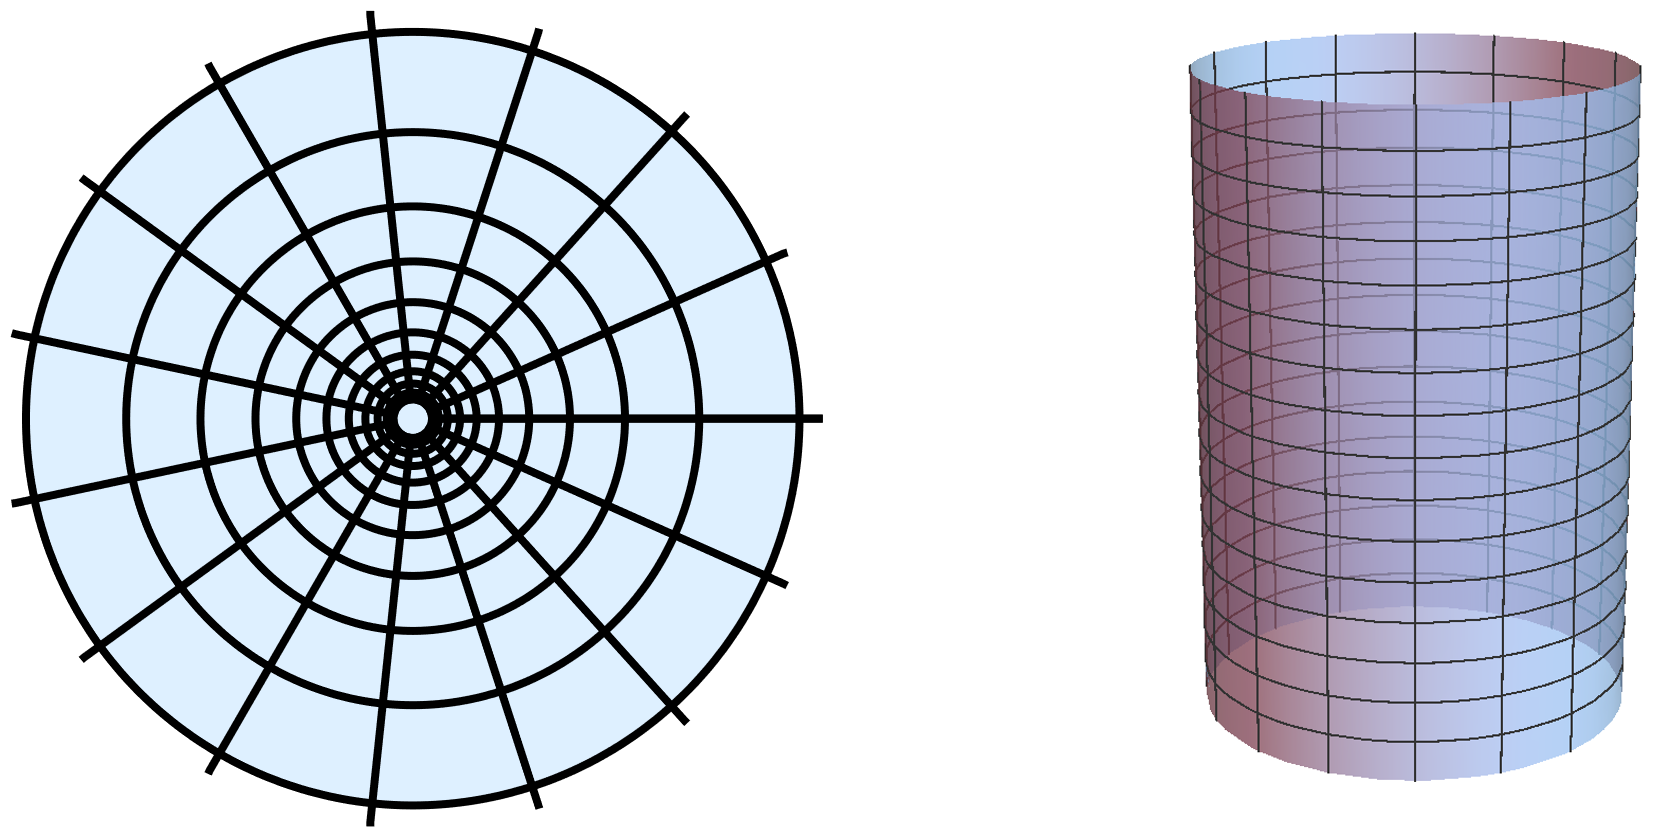
\includegraphics[width=0.72\textwidth]{figures/fig01.png}
  \caption{平面原点处的局域算符，在态-算符对应下映射为圆/柱面上 CFT 的一个态。（原文 p.2，图 1）}
  \label{fig:1}
\end{figure}

在算符乘积展开下，能动张量生成 Virasoro 代数。局域算符空间 $\mathcal{H}$ 构成 Virasoro 代数的一个表示，它可分解为不可约表示的直和，每个不可约表示都含有一个最低维的"原初"算符。

\begin{figure}[htbp]
  \centering
  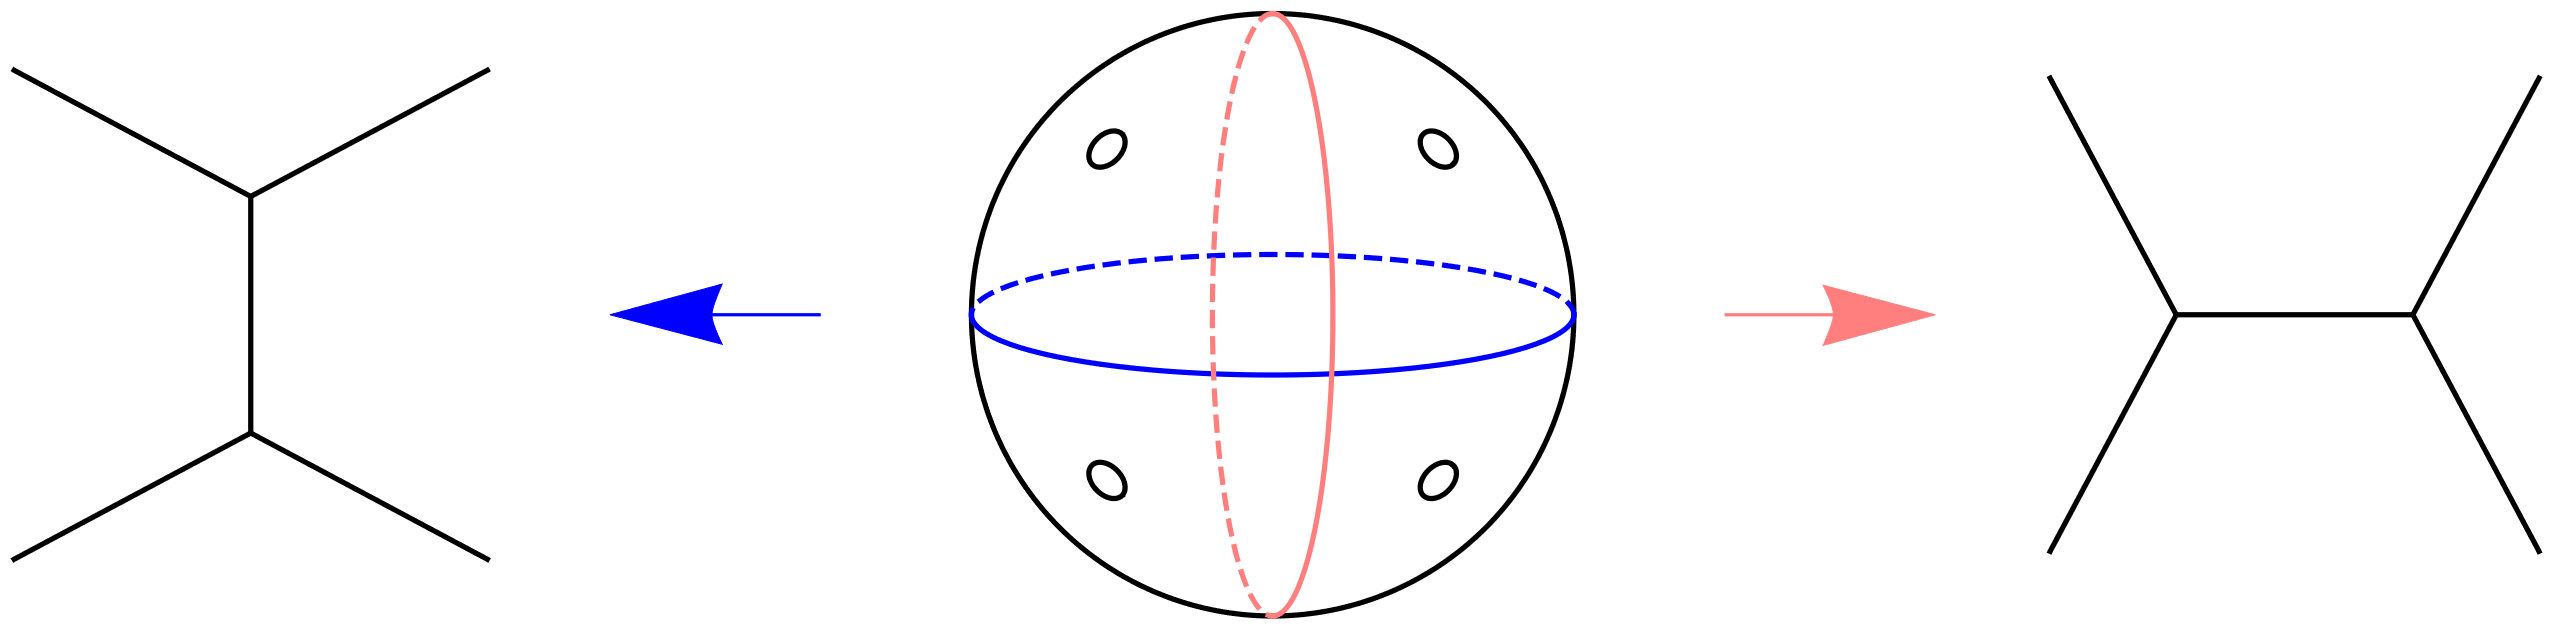
\includegraphics[width=0.92\textwidth]{figures/fig02.png}
  \caption{OPE 的结合性等价于球面四点函数的交叉对称性。（原文 p.2，图 2）}
  \label{fig:2}
\end{figure}

\begin{figure}[htbp]
  \centering
  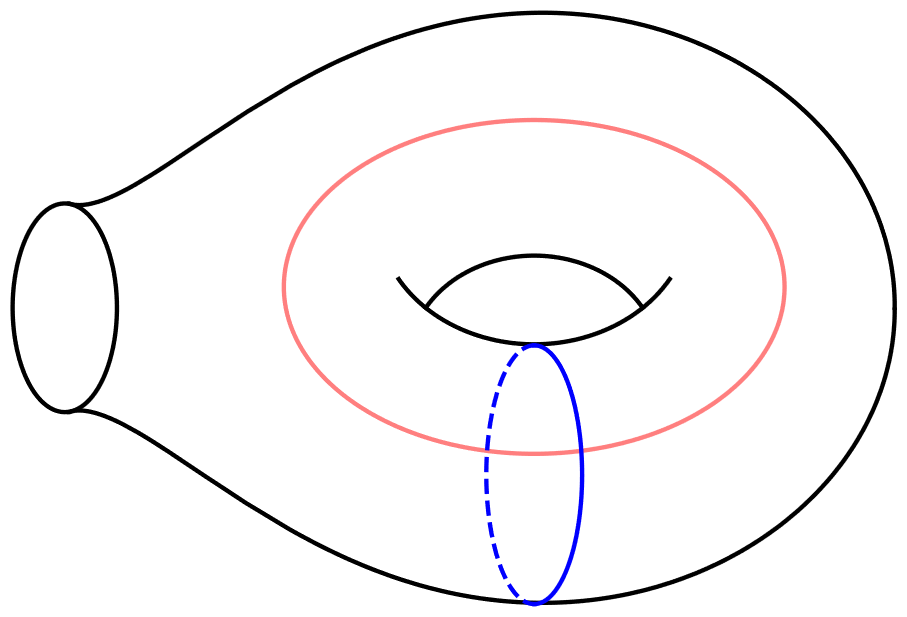
\includegraphics[width=0.40\textwidth]{figures/fig03.png}
  \caption{环面单点函数的模协变性是二维 CFT 的另一条关键自洽性条件。（原文 p.2，图 3）}
  \label{fig:3}
\end{figure}

平面上（或共形等价的黎曼球面上）分离点处的局域算符关联函数有良好定义，且完全由算符乘积展开确定。利用局域算符作为圆周上态的完备性，通过管道化（plumbing）构造，可以在任意黎曼面上构造局域算符的关联函数。二维 CFT 在一般黎曼面上的自洽性要求：由不同"裤子"分解的管道化构造算出的关联函数必须彼此一致。这实际上等价于 OPE 的结合性（球面四点函数的交叉不变性），再加上原初算符环面单点函数的模协变性 \cite{r1}。

\subsection{Virasoro 代数}\label{subsec:2.1}

在欧氏平面上，取复坐标 $(z,\bar z)$，线元为 $\dd s^2=\dd z\,\dd\bar z$。能动张量有两个独立分量：$T(z)\equiv T_{zz}(z)$ 与 $\bar T(\bar z)\equiv T_{\bar z\bar z}(\bar z)$。一对能动张量（比如全纯分量）的 OPE 为
\begin{equation}
  \label{eq:2-1}
  T(z)T(0) \sim \frac{c}{2z^4} + \frac{2}{z^2}T(0) + \frac{1}{z}\partial T(0),
\end{equation}
其中已略去 $z\to0$ 极限下的非奇异项。右端 $z^{-2}$ 阶项由膨胀对称性（其 Noether 流为 $zT(z)$）对应的 Ward 恒等式决定，$z^{-1}$ 阶项则由平移对称性（由 $T(z)$ 生成）对应的 Ward 恒等式决定。假定不存在负维数算符，且唯一的零维算符正比于单位算符，则 (2.1) 就是 $TT$ OPE 最一般的形式（注意 $z^{-3}$ 项会与 OPE 的交换性冲突）。

% [Tutor Note: (2.1) 的三个系数不是独立的：$z^{-4}$ 系数是中心荷 $c/2$，$z^{-2}$ 系数恒为 2，$z^{-1}$ 系数恒为 1，后两者由 $T$ 的维数（2）与 Ward 恒等式固定，不能随意改动。这几个数字是后面所有共形块计算的基准，抄写时极易漏掉因子 2。]

在原点处存在局域算符 $\mathcal{O}(0)$ 时，$T(z)$ 在 $\mathbb{C}\backslash\{0\}$ 上全纯。于是 $T(z)$ 有 Laurent 级数表示
\begin{equation}
  \label{eq:2-2}
  T(z)=\sum_{n=-\infty}^{\infty}\frac{L_n}{z^{n+2}},
  \qquad
  L_n=\oint\frac{\dd z}{2\pi i}\,z^{n+1}T(z),
\end{equation}
该级数在以原点为中心、内部不再插入其他局域算符的圆环上收敛（在关联函数的意义下）。类似地，定义 $\bar L_n$ 为 $\bar T(\bar z)$ 的反全纯 Laurent 系数。$L_n$ 生成中心荷为 $c$ 的 Virasoro 代数
\begin{equation}
  \label{eq:2-3}
  [L_n,L_m]=(n-m)L_{n+m}+\frac{c}{12}(n^3-n)\,\delta_{n,-m},
\end{equation}
同样 $\bar L_n$ 生成另一份 Virasoro 代数，其中心荷 $\tilde c$ 可以不同。

% [Tutor Note: $L_n$ 的定义式 (2.2) 中幂次是 $z^{n+1}$，相应地 $T(z)=\sum L_n z^{-n-2}$；若换成 $z^{-n-2}$ 的另一种约定，对易关系 (2.3) 的 $c$ 项不变但 $n$ 的移位会变。核对后续共形块公式时务必以此处幂次为准。]

一般的无穷小共形变换由 Noether 流
\begin{equation}
  \label{eq:2-4}
  (j_z,j_{\bar z})=\bigl(-\epsilon(z)T(z),\,-\tilde\epsilon(\bar z)\bar T(\bar z)\bigr)
\end{equation}
生成。局域算符 $\mathcal{O}(z,\bar z)$ 的相应变换为
\begin{equation}
  \label{eq:2-5}
  \delta_\epsilon\mathcal{O}(z,\bar z)
  =-\oint_{C_z}\frac{\dd w}{2\pi i}\,\epsilon(w)T(w)\mathcal{O}(z,\bar z)
  +\oint_{C_z}\frac{\dd\bar w}{2\pi i}\,\tilde\epsilon(\bar w)\bar T(\bar w)\mathcal{O}(z,\bar z),
\end{equation}
其中 $C_z$ 是逆时针环绕 $z$ 的围道。特别地，由此可推出能动张量 $T(z)$ 自身的无穷小共形变换：
\begin{equation}
  \label{eq:2-6}
  \delta_\epsilon T(z)=-\frac{c}{12}\partial^3\epsilon(z)-2\partial\epsilon(z)T(z)-\epsilon(z)\partial T(z).
\end{equation}

% [Tutor Note: (2.5) 的围道积分把算符的变换写成"把 $\epsilon T$ 与算符做径向序乘积再取留数"，这正是径向量子化下 Ward 恒等式的标准形式；第二个积分中 $\bar w$ 围道的取向与全纯部分相反，两部分的相对符号是初学者最容易出错的地方。]

把无穷小变换复合起来便得到有限共形变换。用与之相伴的全纯微分同胚来刻画较为方便，其无穷小形式为
\begin{equation}
  \label{eq:2-7}
  z\mapsto z'(z)=z+\epsilon(z).
\end{equation}
过渡到由 $z'=f(z)$ 表示的有限共形变换，$T(z)$ 变换为 $T'(z)$，满足
\begin{equation}
  \label{eq:2-8}
  \left(\frac{\partial z'}{\partial z}\right)^{2}T'(z')=T(z)-\frac{c}{12}\{z',z\},
\end{equation}
其中
$\displaystyle \{z',z\}=\frac{2\partial^3 z'\,\partial z'-3(\partial^2 z')^2}{2(\partial z')^2}$
是 Schwarzian 导数。

% [Tutor Note: Schwarzian 导数的定义各书相差一个整体符号与因子 2；检验约定是否一致的最快办法是取 $z'=z+\epsilon$，(2.8) 应回到 (2.6)。另外 $\{z',z\}$ 对 Möbius 变换 $z'=(az+b)/(cz+d)$ 恒为零，这正是全局共形变换下 $T$ 按张量变换的原因。]

共形变换的一个基本而重要的例子，是从以 $w$ 参数化的欧氏柱面到以 $z$ 参数化的复平面的指数映射 $z=e^{-iw}$：
\begin{equation}
  \label{eq:2-9}
  T_{ww}(w)=(\partial_w z)^2T_{zz}(z)+\frac{c}{24}.
\end{equation}
原点处有算符时 $T_{zz}(z)$ 的 Laurent 展开，此时变为柱面上 $T_{ww}(w)$ 的 Fourier 展开：
\begin{equation}
  \label{eq:2-10}
  T_{ww}(w)=-\sum_{n=-\infty}^{\infty}L_n\,e^{inw}+\frac{c}{24}.
\end{equation}
类似地有
\begin{equation}
  \label{eq:2-11}
  \bar T_{\bar w\bar w}(\bar w)=-\sum_{n=-\infty}^{\infty}\bar L_n\,e^{-in\bar w}+\frac{\tilde c}{24}.
\end{equation}

% [Tutor Note: (2.9) 与 (2.10) 中的常数 $+c/24$ 是柱面上的 Casimir 能，来自 $z=e^{-iw}$ 的 Schwarzian 导数：$\{e^{-iw},w\}$ 给出 $1/2$，乘 $-c/12$ 并补上 $( \partial_w z)^2$ 的贡献后正好是 $c/24$。从 (2.9) 到 (2.10) 只需代入 $z^{-n-2}=e^{i(n+2)w}$ 与 $(\partial_w z)^2=-e^{-2iw}$，读者应亲手验证一次符号。]

记 $w=\sigma+i\tau$，取 $\tau=-it$ 即可解析延拓到洛伦兹号差。如此 $w=\sigma+t$ 与 $\bar w=\sigma-t$ 成为两个独立的实参数。此外，在洛伦兹号差下能动张量分量 $T_{ww}$ 与 $\bar T_{\bar w\bar w}$ 是厄米算符。于是算符 $L_n$ 的厄米共轭为 $L_{-n}$，同样 $\bar L_n^{\dagger}=\bar L_{-n}$。按定义，幺正 CFT 在（洛伦兹）柱面上的态构成全纯与反全纯 Virasoro 代数的幺正表示。

% =====================================================================
%  chapters/ch02b.tex —— 第 2 节后半（原书 p.4--7，PDF 第 5--8 页）
%  2.2 Virasoro 代数的表示 / 2.3 OPE 的结合性 / 2.4 模不变性
%  译者 tr02；体例 work/style_guide.md。
%  公式以 work/pages/page_004.png--page_007.png 为唯一权威；
%  编号公式 label 为 eq:2-12 ... eq:2-26，与原文 (2.12)--(2.26) 一一对应。
%  图 4：figures/fig04.png（原书 p.7）。
%  说明一：本文件不自带 \section，也不写第 2 节的“本节重点”框（由 chapters/ch02.tex
%          的 \section 处统一给出）。
%  说明二：2.4 末句“Namely,”跨页，其续文与式 (2.26) 位于 page_008.png 顶部，
%          为收束第 2 节一并收入；第 3 节及其后的内容不在本文件。
% =====================================================================

\subsection{Virasoro 代数的表示}

以下只讨论 $L_0$ 有下界的 Virasoro 代数表示；一切幺正表示都满足这一性质。这类不可约表示由柱面上的一个原初态 $|h\rangle$ 生成：该态的 $L_0$ 本征值 $h$ 最低，并满足
\begin{equation}
  \label{eq:2-12}
  L_0|h\rangle = h|h\rangle,\qquad L_n|h\rangle = 0,\quad n>0.
\end{equation}
% [Tutor Note: (2.12) 的两条正是“原初态”的定义。$L_n|h\rangle=0$（$n>0$）等价于对应算符在原点正则，即 $T(z)\mathcal{O}_h(0)$ 的 Laurent 展开只含非负幂。柱面上 $L_0$ 与 Hamiltonian 的关系是 $H=\frac{2\pi}{L}\bigl(L_0+\bar L_0-\frac{c}{12}\bigr)$，故“$L_0$ 有下界”就是能量有下界；若去掉这一条，就允许出现 $L_0$ 无下界的表示，这类表示在非幺正的理论中确实存在。]

在态-算符对应下，$|h\rangle$ 对应原点处的原初算符 $\mathcal{O}_h$。原初算符 $\mathcal{O}_h(z)$（以下省略反全纯依赖）在一般共形变换下的变换律为
\begin{equation}
  \label{eq:2-13}
  \mathcal{O}'_h(z') = (\partial_z z')^{-h}\,\mathcal{O}_h(z).
\end{equation}
% [Tutor Note: 权 $(h,\bar h)$ 的原初场变换律是 $(\partial_z z')^{-h}(\partial_{\bar z}\bar z')^{-\bar h}$，原文此处只写全纯部分。指数是 $-h$ 而非 $-1$，因子中不含 $c$；与能动张量的变换律（含 Schwarzian 导数项）相比，原初场没有这些附加项，这正是“原初”与准原初的分界。]

Virasoro 后代的一般基矢取为
\begin{equation}
  \label{eq:2-14}
  L_{-N}|h\rangle \equiv L_{-n_1}\cdots L_{-n_k}|h\rangle,
\end{equation}
% [Tutor Note: 原文紧邻处有两处英文拼写笔误：正文 "A basis for the general Viraosro descendants"（应为 Virasoro），以及上一段 "omitted anti-holormophic dependence"（应为 anti-holomorphic）。译文按正字处理，公式与含义不受影响，此处留档备校勘。]

其中 $N$ 记整数分拆 $\{n_1,n_2,\cdots,n_k\}$，约定按降序排列 $n_1\ge n_2\ge\cdots\ge n_k\ge 1$。称 $|N|=\sum_{j=1}^{k}n_j$ 为该状态的能级。第 $n$ 能级的 Gram 矩阵定义为该能级各基矢内积构成的矩阵：
\begin{equation}
  \label{eq:2-15}
  G^{(n)}_{NM} = \langle h|L_{-N}^{\dagger}L_{-M}|h\rangle,\qquad |N|=|M|=n,
\end{equation}
归一化约定取 $\langle h|h\rangle=1$。矩阵元 $G^{(n)}_{NM}$ 是 $c$ 与 $h$ 的多项式函数。最受关注的是 $G^{(n)}$ 的行列式，即 Kac 行列式，其公式（见 \cite{r2,r3}）为
\begin{equation}
  \label{eq:2-16}
  \det G^{(n)} = K_n\prod_{1\le rs\le n}(h-h_{r,s})^{P(n-rs)}.
\end{equation}
这里 $K_n$ 是正的常数，$P(m)$ 是分拆数，满足 $\sum_{m=0}^{\infty}P_m q^m=\prod_{k=1}^{\infty}(1-q^k)^{-1}$；$h_{r,s}$ 由下式给出
% [Tutor Note: 原句把分拆数生成函数写成 $\sum_m P_m q^m$（下标 $m$），而同句前面定义的是 $P(m)$；两种记号在同一句内混用，图像上确实如此，译文照原样排。另注意 (2.16) 的乘积遍历满足 $rs\le n$ 的整数对 $(r,s)$，$P(n-rs)$ 是幂次而不是求和指标；$K_n$ 是与 $h$ 无关的正的归一化常数，其具体值由 Gram 矩阵的归一化决定。]
\begin{equation}
  \label{eq:2-17}
  h_{r,s} = \frac{c-1}{24}+\frac{1}{4}(r\alpha_+ + s\alpha_-)^2,\qquad
  \alpha_\pm = \frac{\sqrt{1-c}\pm\sqrt{25-c}}{\sqrt{24}}.
\end{equation}
% [Tutor Note: 核对 (2.17) 时注意根号的分支：$c>1$ 时 $\sqrt{1-c}=i\sqrt{c-1}$；$c>25$ 时两根号都是纯虚，$h_{r,s}$ 为实数且非正。原文说 $1<c<25$ 时 $h_{r,s}$ 为复数，严格讲这只对 $r\ne s$ 成立：$r=s$ 时 $r\alpha_++s\alpha_-=2ir\sqrt{c-1}/\sqrt{24}$，由 (2.17) 得 $h_{r,r}=(c-1)(1-r^2)/24\le 0$，仍是实数，不在正实轴上，下文论证不受影响。]
后面还会用到 $c=1+6Q^2$、$Q\equiv b+b^{-1}$ 的定义，此时可把 $h_{r,s}$ 改写成
\begin{equation}
  \label{eq:2-18}
  h_{r,s} = \frac{Q^2}{4}-\frac{1}{4}(rb+sb^{-1})^2.
\end{equation}
% [Tutor Note: 由 $Q=b+b^{-1}$ 且 $b$ 为实数得 $Q^2\ge 4$，故 $c=1+6Q^2\ge 25$，等号仅在 $b=\pm1$（此时 $Q=\pm2$、$\alpha_\pm=i$）成立。原文写 “$c>25$” 略欠精确，应理解为 $c\ge 25$；这与后文按 $c\ge 25$ 分类的说法一致。]
注意：对实数 $b$，有 $c>25$，且 $\alpha_\pm$ 为纯虚数。

式 \eqref{eq:2-16} 背后的直观是：权为 $h=h_{r,s}$ 的原初态 $V_h$ 在第 $rs$ 能级上有一个零 Virasoro 后代，可写成如下形式
\begin{equation}
  \label{eq:2-19}
  \chi_{rs} = \sum_{|N|=rs}\chi_{rs}^{N}L_{-N}V_{h_{rs}},
\end{equation}
其中系数 $\chi_{rs}^{N}$ 归一化取为 $\chi_{rs}^{\{1,\cdots,1\}}=1$。在更高能级 $n>rs$ 上，形如 $L_{-M}\chi_{rs}$（$|M|=n-rs$）的后代共有 $P(n-rs)$ 个，它们同样具有零模长，于是 Kac 行列式出现 $P(n-rs)$ 阶零点。
% [Tutor Note: 归一化条件 $\chi_{rs}^{\{1,\cdots,1\}}=1$ 是取 $\chi_{rs}$ 中 $L_{-1}^{rs}V_{h_{rs}}$ 这一项的系数为 1；其余系数由“$\chi_{rs}$ 是第 $rs$ 能级 Gram 矩阵的零本征矢量”即 $L_n\chi_{rs}=0$（$n>0$）这组线性条件定出（这正是奇异矢量的构造）。$\chi_{rs}$ 的模长为零，故它不贡献新的物理态。]
由 $h_{1,1}=0$ 可知，幺正表示必须有 $h\ge 0$（$h=0$ 对应单位算符/真空表示）。若 $c>1$，$h_{r,s}$ 或为非正实数（$c\ge 25$ 时），或为复数（$1<c<25$ 时）；而 $\det G^{(n)}$ 作为 $h$ 的实函数不可能在正实轴上取零，故对一切 $h>0$ 必须为正。

若 $c=1$，$\det G^{(n)}$ 对 $h\ge 0$ 非负，但它在正实轴上确有零点，因为部分 $h_{r,s}$ 为正实数；这些零点对应 $c=1$ 的 Virasoro 代数表示中的零态。

若 $c<1$，可以证明：只要 $h$ 不等于某个 $h_{r,s}$，$\det G^{(n)}$ 就会对某个 $n$ 取负值。细致的分析给出 $c<1$ 时可能存在的离散幺正表示 \cite{r4,r5}：
\begin{equation}
  \label{eq:2-20}
  c = 1-\frac{6}{m(m+1)},\qquad
  h = h_{r,s} = \frac{\bigl((m+1)r-ms\bigr)^2-1}{4m(m+1)}
  \quad\text{with } 1\le r\le m-1,\ 1\le s\le m,
\end{equation}
其中 $m=2,3,\cdots$。
% [Tutor Note: (2.20) 中 $(r,s)$ 与 $(m-r,\,m+1-s)$ 给出同一个 $h$，因为 $(m+1)(m-r)-m(m+1-s)=-[(m+1)r-ms]$；故独立的 $h$ 只有表中一半，即 $m(m-1)/2$ 个，这正是极小模型里原初场的个数。另注意此处的 $m$ 与 (2.16) 中分拆数 $P(m)$ 的 $m$ 是两个不同的量，只是碰巧用同一字母。]

\subsection{OPE 的结合性}

算符乘积展开的一般形式为
\begin{equation}
  \label{eq:2-21}
  \mathcal{O}_i(z_1,\bar z_1)\mathcal{O}_j(z_2,\bar z_2)
  = \sum_k A_{ij}^{k}(z_{13},z_{23};\bar z_{13},\bar z_{23})\,\mathcal{O}_k(z_3,\bar z_3),
\end{equation}
其中求和遍历 CFT 中的所有算符，用指标 $k$ 标记。在 $z_3$ 附近作重标度 $z_{i3}\to\lambda z_{i3}$、$\bar z_{i3}\to\bar\lambda\bar z_{i3}$ 时，系数 $A_{ij}^{k}$ 的标度为 $\lambda^{h_k-h_i-h_j}\bar\lambda^{\bar h_k-\bar h_i-\bar h_j}$。式 \eqref{eq:2-21} 作为算符等式，只在代入关联函数之后成立；此时 $z_{i3}$ 与 $\bar z_{i3}$ 的展开有收敛半径 $R$，它由“以 $z_3$ 为心、半径为 $R$ 的圆盘内没有其他算符”这一性质确定。这并不意味着 OPE 在收敛半径之外完全不能用，而是说必须适当重排基 $\mathcal{O}_k$，才能使展开在关联函数中有良好定义。稍后我们会借助共形块的解析延拓更精确地刻画这一点。
% [Tutor Note: 原文在此把反全纯权写作 $\bar h$（$\lambda^{h_k-h_i-h_j}\bar\lambda^{\bar h_k-\bar h_i-\bar h_j}$），到 (2.23)–(2.24) 又改写作 $\tilde h$；这是原文记号不统一，二者指同一个量，译文照原样保留。收敛半径 $R$ 的判据是：$R$ 等于 $z_3$ 到其它算符插入点的最小距离，OPE 只能在这样的圆盘内逐项收敛。]

下面考虑三个算符的乘积，
\begin{equation}
  \label{eq:2-22}
  \mathcal{O}_i(z_1,\bar z_1)\,\mathcal{O}_j(z_2,\bar z_2)\,\mathcal{O}_k(z_3,\bar z_3).
\end{equation}
可以先取 $\mathcal{O}_i\mathcal{O}_j$ 的 OPE，在 $z_4$ 附近展开为 $\mathcal{O}_m(z_4)$，再取 $\mathcal{O}_m(z_4)$ 与 $\mathcal{O}_k(z_3)$ 的 OPE；条件是 $z_4$ 取得合适，使 $|z_{34}|>\max\{|z_{14}|,|z_{24}|\}$。也可以先取 $\mathcal{O}_j\mathcal{O}_k$ 的 OPE，在 $z_5$ 附近展开为 $\mathcal{O}_n(z_5)$，再取 $\mathcal{O}_i(z_1)$ 与 $\mathcal{O}_n(z_5)$ 的 OPE；条件是 $|z_{15}|>\max\{|z_{25}|,|z_{35}|\}$。按构造，这两种展开应给出同一结果，由此得到系数 $A_{ij}^{k}$ 的一组相容性条件。

充分利用共形对称性的办法，是按原初算符与后代来组织 OPE。例如一对原初算符的 OPE 取如下形式
\begin{equation}
  \label{eq:2-23}
  \begin{aligned}
  \phi_i(z_1,\bar z_1)\,\phi_j(z_2,\bar z_2)
  ={}& \sum_k C_{ij}^{k}\sum_{N,M}
  B_N(h_i,h_j;h_k|z_{13},z_{23})\\
  &\times B_M(\tilde h_i,\tilde h_j;\tilde h_k|\bar z_{13},\bar z_{23})\,
  L_{-N}\bar L_{-M}\phi_k(z_3,\bar z_3),
  \end{aligned}
\end{equation}
其中求和遍历原初算符 $\phi_k$，以及标记全纯与反全纯 Virasoro 后代的整数分拆 $N,M$。函数 $B_N(h_i,h_j;h_k|z_{13},z_{23})$ 完全由共形 Ward 恒等式确定，只依赖进入 Virasoro 代数的中心荷 $c$。系数 $C_{ij}^{k}$ 是结构常数。
% [Tutor Note: (2.23) 中 $L_{-N}$ 与 $\bar L_{-M}$ 都作用在同一个 $\phi_k(z_3,\bar z_3)$ 上，且 $N$ 与 $M$ 独立求和；$B_N$ 只含全纯数据 $(h_i,h_j,h_k;z_{13},z_{23})$，$B_M$ 只含反全纯数据。$B_N$ 由共形 Ward 恒等式递推定死（依赖 $c$），这正是下一节共形块递推表示的出发点。]
若把原初算符的基 $\phi_k$ 归一化为如下二点函数（在平面或黎曼球面上）
\begin{equation}
  \label{eq:2-24}
  \langle\phi_i(z_1,\bar z_1)\,\phi_j(z_2,\bar z_2)\rangle
  = \frac{\delta_{ij}}{z_{12}^{2h_i}\,\bar z_{12}^{2\tilde h_i}},
\end{equation}
% [Tutor Note: (2.24) 分母的指数是 $2h_i$ 与 $2\tilde h_i$（不是 $h_i$ 与 $\tilde h_i$）：权 $(h_i,\bar h_i)$ 的原初场二点函数由共形对称性唯一确定为 $z_{12}^{-2h_i}\bar z_{12}^{-2\bar h_i}$，$\delta_{ij}$ 来自不同原初场的正交性。只有取此归一化，$C_{ijk}$ 才对三个指标完全对称；若各场重新标度，对称性会被各自的归一化因子破坏。]
则 $C_{ijk}=C_{ij}^{k}$ 就是三点函数 $\langle\phi_i\phi_j\phi_k\rangle$ 的系数，并且对 $i,j,k$ 完全对称。

原初算符集合 $\phi_i$ 连同结构常数 $C_{ijk}$ 一起确定了算符乘积代数，从而确定平面或球面上的一切关联函数。由于 OPE 的结合性，它们受到极强的非平凡约束，这一点后面再展开。

\subsection{模不变性}

二维黎曼流形都是共形平坦的，因此二维 CFT 可以典范地定义在任意黎曼面上，只差一个普适的共形反常：它使结果依赖共形类内部度规的选取。此外，对给定的 CFT，任意一组局域算符插入一般黎曼面所得的关联函数，都由结构常数 $C_{ijk}$ 经管道化构造确定。同一黎曼面可以由不同的管道化构造得到；CFT 在这些构造下的一致性给出一组重要的相容条件，称为模不变性。\footnote{一个很有意思的公开问题是：模不变性与“分裂性质”意义下的局域希尔伯特空间这一概念之间有何关系 \cite{r6,r7}。}
% [Tutor Note: 这里的“普适的共形反常”指 Weyl 变换的量子反常 $T^\mu_{\ \mu}=\frac{c}{12}R$（反全纯部分系数为 $\bar c$）：$c$ 只由 CFT 本身决定，与具体黎曼面无关，因此配分函数在同一共形类内只通过度规的选取（即模参数）体现依赖。]
% [Tutor Note: “分裂性质”（split property）是局域代数量子场论中的一条性质：若两块区域相距正距离，则各自可观测量代数生成的 von Neumann 代数自然同构于两者的张量积，于是整体希尔伯特空间可作局域分解。原文把模不变性与这一“局域希尔伯特空间”概念的关系列为公开问题。]

作为光滑流形，亏格 $g$ 的曲面可由“裤子”（pair-of-pants，即三孔球面）粘合而成。一般的 $g>1$ 黎曼面可由 $2g-2$ 个三孔球面管道化拼接得到。亏格为 1 的情形则由一个圆环的内外边界管道化拼接得到。管道化构造用 $PSL(2,\mathbb{C})$ 映射把三孔球面（或双孔圆盘）的一对圆形边界粘在一起。典型的管道化映射形如
\begin{equation}
  \label{eq:2-25}
  z' = q/z,\qquad q\in\mathbb{C}^{\times},
\end{equation}
它把其中一个双孔圆盘的边界 $|z|=r_1$ 与另一个双孔圆盘的边界 $|z'|=r_2$ 等同起来，并有 $r_1r_2=|q|$。每个管道化映射对应一个复模 $q$；$3g-3$ 个管道化映射给出黎曼面的 $3g-3$ 个复结构模。
% [Tutor Note: 由 $z'=q/z$ 立即得 $|z'|=|q|/|z|$，故把 $|z|=r_1$ 映到 $|z'|=r_2$ 要求 $r_1r_2=|q|$。亏格 1 时粘合的是同一圆环的内外边界，此时 $q$ 与模参数的关系为 $q=e^{2\pi i\tau}$；注意这套 $q,\tau$ 参数与柱面上 Fourier 展开的 $e^{inw}$（见 2.1 节）是两套不同的量，后文推导环面配分函数时不可混用。]

\begin{figure}[htbp]
  \centering
  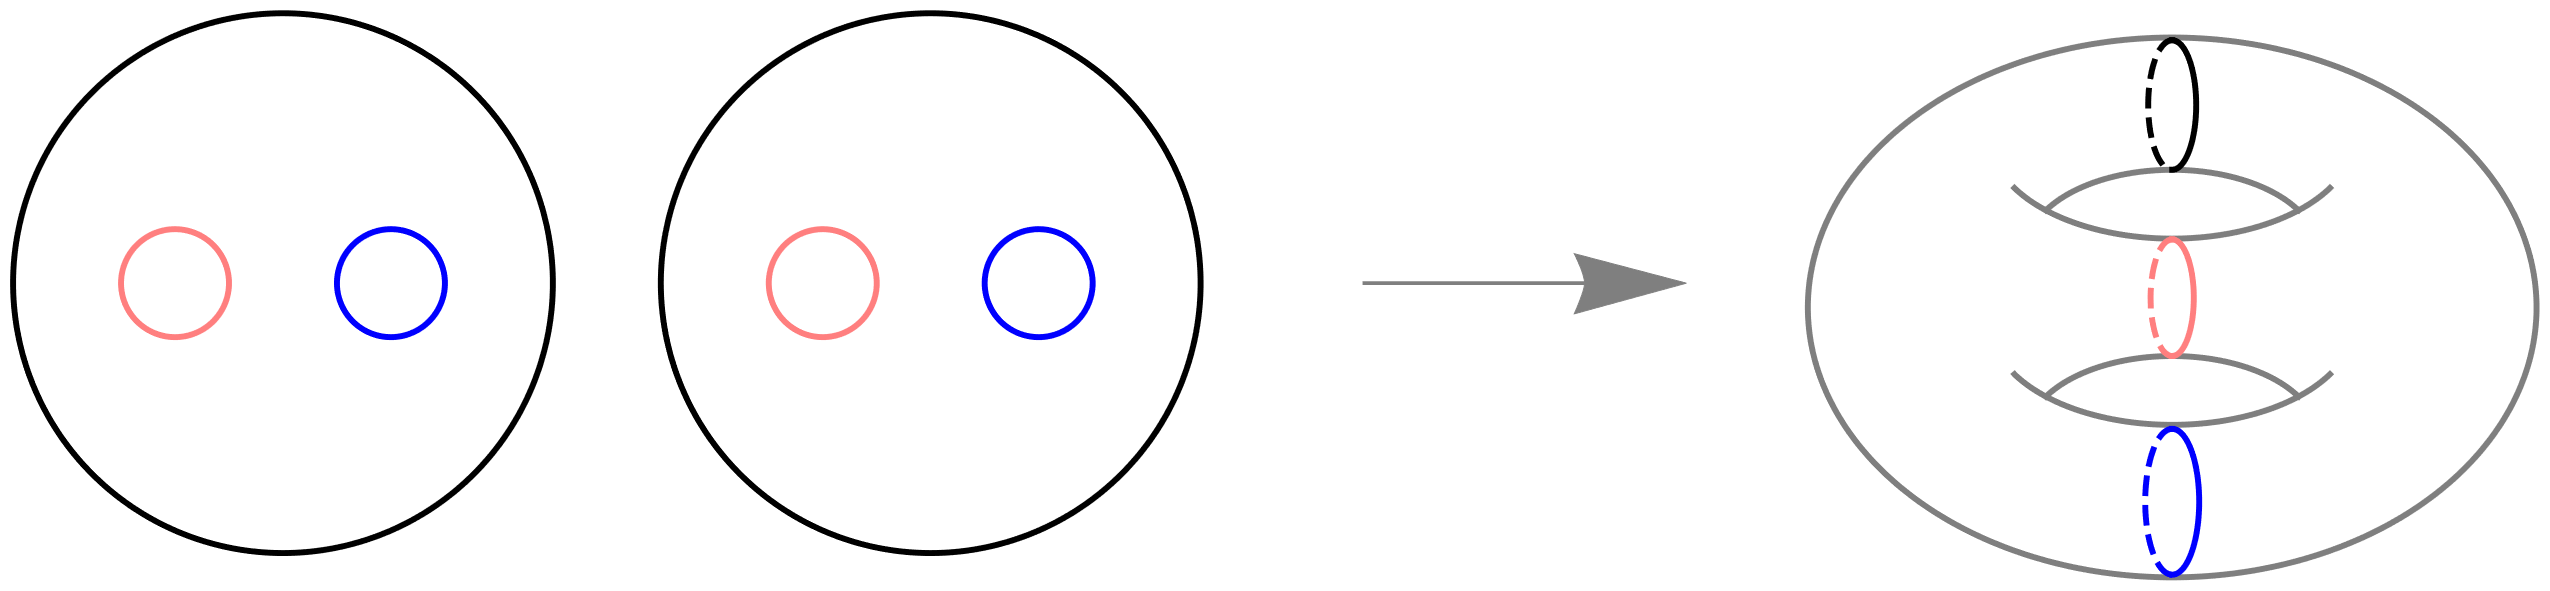
\includegraphics[width=0.85\textwidth]{figures/fig04.png}
  \caption{亏格 2 黎曼面的管道化构造：两个三孔球面（左、中）经三根管道（右）粘合；三根管道正对应 $3g-3=3$ 个复模。（原文 p.7，图 4）}
  \label{fig:4}
\end{figure}
% [Tutor Note: 数目要与图 4 对照看：$g=2$ 时 $2g-2=2$ 个三孔球面、$3g-3=3$ 个管道化映射，图 4 右侧就是两个三孔球面之间连三根管道。$3g-3$ 同时是亏格 $g$ 黎曼面模空间的复维数，故每根管道恰好贡献一个复模 $q$；$g=1$ 时 $3g-3=0$，只余一个复模 $\tau$，与环面情形相符。]

管道化构造给出一种精确的办法，在任意亏格 $g$ 的黎曼面上构造配分函数，更一般地构造关联函数。出发点是黎曼球面上任意 Virasoro 后代的三点函数，而三点函数由共形 Ward 恒等式用结构常数 $C_{ijk}$ 确定。所谓模不变性，就是断言：同一（带穿孔的）黎曼面的所有可能管道化构造，都给出相同的配分函数（关联函数）。

同一黎曼面的不同管道化构造之间等价，只需以下两条成立：所有球面四点函数都能等价地在两个不同通道中分解；由带一个穿孔的圆环内外边界管道化得到的全部环面一点函数，与把环面剪开成圆环的方式无关。前者正是前面已经提到的 OPE 结合性；后者等价于所有原初算符的环面一点函数具有模协变性。具体说来，对每个原初算符 $\phi_k(z,\bar z)$，环面一点函数 $\langle\phi_k(z,\bar z)\rangle_{T^2(\tau)}=f_k(\tau,\bar\tau)$ 是权为 $(h_k,\tilde h_k)$ 的模形式。也就是说，
\begin{equation}
  \label{eq:2-26}
  f_k(\tau+1,\bar\tau+1)=f_k(\tau,\bar\tau),\qquad
  f_k(-1/\tau,-1/\bar\tau)=(-i\tau)^{h_k}(i\bar\tau)^{\tilde h_k}f_k(\tau,\bar\tau).
\end{equation}
% [Tutor Note: (2.26) 是权 $(h_k,\tilde h_k)$ 模形式的定义：$T:\tau\to\tau+1$ 下不变，$S:\tau\to-1/\tau$ 下带自守因子 $(-i\tau)^{h_k}(i\bar\tau)^{\tilde h_k}$。环面一点函数与插入点 $z$ 无关，是因为环面上的平移 Killing 矢量使 $\langle\phi_k(z)\rangle$ 为常数，这对原初场成立。$S$ 变换中 $(-i\tau)^{h_k}$ 的 $i$ 相位与幂次是这一段里最易写错处，务必与 $q=e^{2\pi i\tau}$ 的约定一起核对。]

% =====================================================================
% ch03a.tex —— 第 3 节前半（PDF p.9–13，原书 p.8–12）
% 译者：tr03a；体例见 work/style_guide.md
% 底本：Xi Yin, Aspects of 2D CFTs, PoS(TASI2017)003
% =====================================================================

\section{Virasoro 共形块}\label{sec:3}

\begin{keytakeaways}
  \item 核心物理图像：球面四点函数按 OPE 通道 $12\to 34$ 分解，每个共形块收集中间原初场及其全部 Virasoro 后代的贡献。
  \item 使用的数学工具：共形 Ward 恒等式、Virasoro 后代 Gram 矩阵之逆 $G^{NM}(c,h)$、Kac 行列式的零点、超几何函数。
  \item 本节结论：共形块在 $|z|<1$ 内收敛；它在 $h$ 平面与 $c$ 平面的极点位置由 Kac 行列式给出，留数由融合多项式与低一阶共形块表示，由此得到递推表示。
\end{keytakeaways}

我们首先考虑球面上原初场 $\phi_i(z_i,\bar z_i)$ 的四点函数，其中 $i=1,2,3,4$。如前所见，若把 $\phi_i$ 两两的算符乘积展开（OPE）写成对一整组原初场的 Virasoro 后代求和，四点函数便由共形 Ward 恒等式用结构常数 $C_{12k},C_{34k}$ 确定。下面具体做这个计算。利用黎曼球的共形 Killing 群 $PSL(2,\mathbb{C})$，可以把四个算符放在
\begin{equation}\label{eq:3-1}
  z_1=0,\qquad z_2=z,\qquad z_3=1,\qquad z_4=\infty .
\end{equation}

为使关联函数有限且定义良好，在 $z_4\to\infty$ 极限下对 $\phi_4(z_4,\bar z_4)$ 作重标度，定义为
\begin{equation}\label{eq:3-2}
  \phi_4'(\infty)=\lim_{z_4,\bar z_4\to\infty} z_4^{2h_4}\bar z_4^{2\tilde h_4}\phi_4(z_4,\bar z_4).
\end{equation}

% [Tutor Note: (3.2) 中 $\phi_4'(\infty)$ 的撇号表示重标度后的算符，不是对 $z$ 求导。指数取 $2h_4$ 而非 $h_4$，来自反演 $z\to 1/z$ 的 Jacobian 因子 $(dz'/dz)^{-h_4}=(-z^{-2})^{-h_4}\sim z^{2h_4}$；再乘上反全纯部分 $\bar z_4^{2\tilde h_4}$，极限才有限。]

现在可以计算关联函数
\begin{equation}\label{eq:3-3}
  \langle\phi_1(0)\phi_2(z,\bar z)\phi_3(1)\phi_4'(\infty)\rangle .
\end{equation}

在径向量子化下，可把 $\phi_1(0)$ 与 $\phi_4'(\infty)$ 分别看作 ket 与 bra，四点函数于是等价地写成
\begin{equation}\label{eq:3-4}
  \langle\phi_4|\phi_3(1)\phi_2(z,\bar z)|\phi_1\rangle .
\end{equation}

\begin{figure}[htbp]
  \centering
  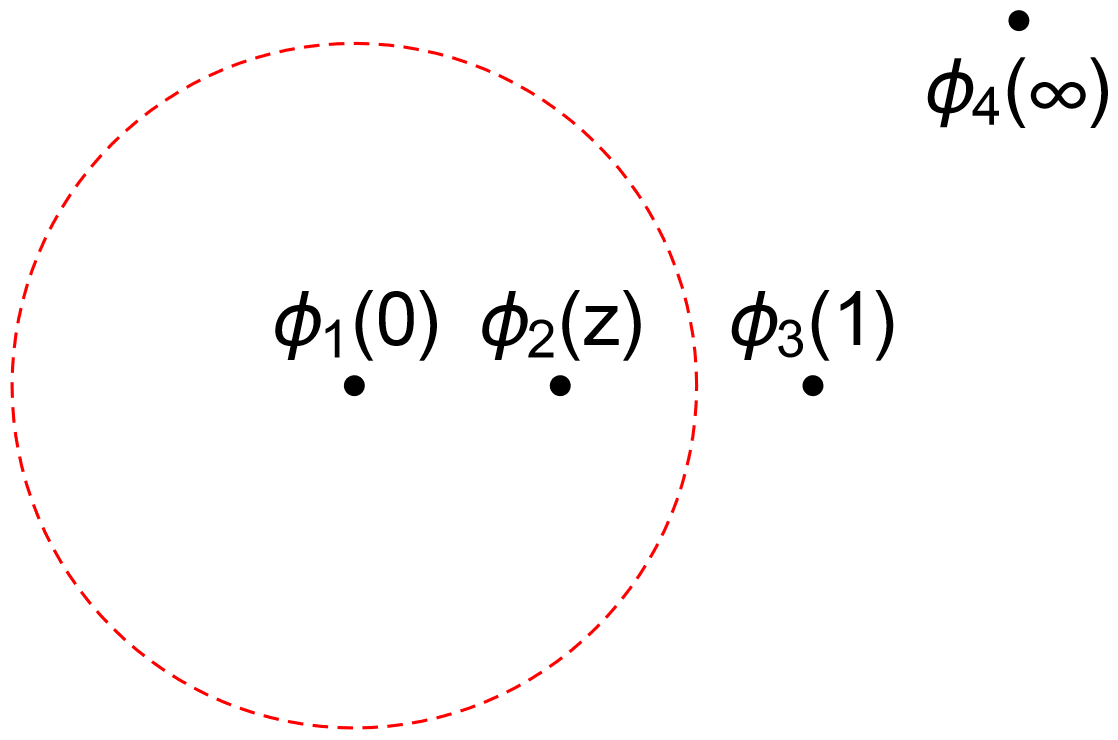
\includegraphics[width=0.85\textwidth]{figures/fig05.png}
  \caption{在四点函数中插入一组完备的态基（红色虚线圈）。（原文 p.8，图 5）}
  \label{fig:5}
\end{figure}

把 $\phi_1\phi_2$（或 $\phi_3\phi_4$）作 OPE，等价于在 \eqref{eq:3-4} 的径向量子化中插入一组完备的态基，这组态基可整理成对 Virasoro 后代的求和：
\begin{equation}\label{eq:3-5}
  \begin{aligned}
    &\langle\phi_4|\phi_3(1)\phi_2(z,\bar z)|\phi_1\rangle\\
    &=\sum_{k}\sum_{|N|=|M|,\,|\tilde N|=|\tilde M|}
    \langle\phi_4|\phi_3(1)L_{-N}\bar L_{-\tilde N}|\phi_k\rangle
    G^{NM}(c,h_k)G^{\tilde N\tilde M}(c,\tilde h_k)
    \langle\phi_k|L^\dagger_{-M}\bar L^\dagger_{-\tilde M}\phi_2(z,\bar z)|\phi_1\rangle ,
  \end{aligned}
\end{equation}
其中 $G^{NM}(c,h)$ 是权重为 $h$ 的原初场的 Virasoro 后代所构成 Gram 矩阵之逆的矩阵元。利用三点函数的伸缩对称性，有
\begin{equation}\label{eq:3-6}
  \begin{aligned}
    &\langle\phi_k|L^\dagger_{-M}L^\dagger_{-\tilde M}\phi_2(z,\bar z)|\phi_1\rangle\\
    &=z^{-h_1-h_2+h_k+|M|}\,
      \bar z^{-\tilde h_1-\tilde h_2+\tilde h_k+|\tilde M|}
      \langle\phi_k|L^\dagger_{-M}\bar L^\dagger_{-\tilde M}\phi_2(1)|\phi_1\rangle .
  \end{aligned}
\end{equation}

% [Tutor Note: (3.6) 左端第二个算符原文写作 $L^\dagger_{-\tilde M}$，右端则写作 $\bar L^\dagger_{-\tilde M}$。按 (3.5) 的记号，反全纯部分应带横杠，此处应是原文排版遗漏。另请注意 $|M|$、$|\tilde M|$ 是分拆的大小（后代层次），不是模长。]

% [Tutor Note: (3.7) 第一行原文把 $\rho$ 的三个宗量全写成带波浪号的 $\tilde v_4,\tilde v_3,\tilde v_k$，并且只出现一个 $\rho$；但 (3.8) 的分解是 $\mathcal F_c\bar{\mathcal F}_c$，应当同时含全纯与反全纯两个因子。译文照原文排，此处疑为原文笔误。]

进一步，我们写
\begin{equation}\label{eq:3-7}
  \begin{aligned}
    \langle\phi_4|\phi_3(1)L_{-N}\bar L_{-\tilde N}|\phi_k\rangle
    &=C_{43k}\,\rho(\tilde v_4,\tilde v_3,\bar L_{-\tilde N}\tilde v_k),\\
    \langle\phi_k|L^\dagger_{-M}\bar L^\dagger_{-\tilde M}\phi_2(1)|\phi_1\rangle
    &=C_{k21}\,\rho(L_{-M}v_k,v_2,v_1)\,
      \rho(\bar L_{-\tilde M}\tilde v_k,\tilde v_2,\tilde v_1),
  \end{aligned}
\end{equation}
其中 $v_i$ 与 $\tilde v_i$ 分别表示权重为 $h_i$ 与 $\tilde h_i$ 的全纯、反全纯 Virasoro 原初场，$\rho(\xi_3,\xi_2,\xi_1)$ 表示剥去结构常数后的 Virasoro 后代 $\xi_i$ 三点函数。特别地，$\rho(\xi_3,\xi_2,\xi_1)$ 完全由共形 Ward 恒等式用 Virasoro 后代 $\xi_i$ 与中心荷 $c$ 确定。于是可把 \eqref{eq:3-5} 写成
\begin{equation}\label{eq:3-8}
  \langle\phi_4|\phi_3(1)\phi_2(z,\bar z)|\phi_1\rangle
  =\sum_k C_{43k}C_{k21}\,
  \mathcal F_c(h_1,h_2,h_3,h_4,h_k;z)\,
  \overline{\mathcal F}_c(\tilde h_1,\tilde h_2,\tilde h_3,\tilde h_4,\tilde h_k;\bar z),
\end{equation}
其中
\begin{equation}\label{eq:3-9}
  \mathcal F_c(h_1,h_2,h_3,h_4,h_k;z)
  =\sum_{|N|=|M|} z^{-h_1-h_2+h_k+|N|}
  \rho(v_4,v_3,L_{-N}v_k)\,
  G^{NM}(c,h_k)\,\rho(L_{-M}v_k,v_2,v_1)
\end{equation}
是 $12\to 34$ OPE 通道中球面四点函数的全纯 Virasoro 共形块。

到目前为止，我们把 $\mathcal F_c$ 定义成 $z$ 的级数展开。$z$ 展开的收敛半径为 $1$，因为 $\mathcal F_c(z)$ 在 $z=1$ 处有（对数）奇点。可以把 $\mathcal F_c(z)$ 解析延拓到整个复 $z$ 平面，支割线从 $z=1$ 延伸到 $z=\infty$。$\mathcal F_c(z)$ 的解析结构将在后文详细讨论。

\subsection{递推表示}\label{sec:3-1}

作为一个简单例子，我们来计算 $\rho(v_1,v_2,L_{-N}v_k)$，取整数分拆 $N$ 只含一个元素 $N=\{n\}$ 的特殊情形，此时 $L_{-N}$ 只涉及单个 Virasoro 生成元 $L_{-n}$，$n\ge 1$。

% [Tutor Note: 原文此处作 "a singular Virasoro generator"；由上下文（$N=\{n\}$ 只含一个元素，故 $L_{-N}=L_{-n}$ 只是单个生成元）判断，singular 应为 single 之误。译文按 single 处理，提请校对复核。]

有
\begin{equation}\label{eq:3-10}
  \begin{aligned}
    \rho(v_1,v_2,L_{-n}v_k)
    &=\langle v_1'(\infty)v_2(1)L_{-n}v_k(0)\rangle
     =\oint_{C_0}\frac{dz}{2\pi i}\,z^{-n+1}
      \langle v_1'(\infty)v_2(1)T(z)v_k(0)\rangle\\
    &=-\oint_{C_\infty}\frac{dz}{2\pi i}\,z^{-n+1}
      \langle v_1'(\infty)v_2(1)T(z)v_k(0)\rangle
     -\oint_{C_1}\frac{dz}{2\pi i}\,z^{-n+1}
      \langle v_1'(\infty)v_2(1)T(z)v_k(0)\rangle\\
    &=\langle (L_n v_1)'(\infty)v_2(1)v_k(0)\rangle
     -\langle v_1'(\infty)\bigl[h_2(-n+1)v_2(1)-\partial v_2(1)\bigr]v_k(0)\rangle\\
    &=\bigl[h_2(n-1)-h_2-h_k+h_1\bigr]\rho(v_1,v_2,v_k)
     =h_2(n-1)-h_2-h_k+h_1 .
  \end{aligned}
\end{equation}
其中 $C_0$ 与 $C_1$ 分别是围绕 $0$ 与 $1$ 的小逆时针围道，而 $C_\infty$ 是一个大的顺时针围道。

% [Tutor Note: (3.10) 第二行的围道变形用 $\oint_{C_0}=-\oint_{C_\infty}-\oint_{C_1}$；$C_\infty$ 已规定为顺时针，故显式带负号。$C_\infty$ 上的积分把 $L_n$ 作用到无穷远处的 $v_1$ 上，得到第三行的 $\langle (L_nv_1)'v_2v_k\rangle$；这正是 $L_n=\oint_{C_0}\frac{dz}{2\pi i}z^{n+1}T(z)$ 在 $z\to1/w$ 下的等价写法，符号最易出错。]

让我们再做一个例子，
\begin{equation}\label{eq:3-11}
  \begin{aligned}
    \rho(L_{-n}v_k,v_2,v_1)
    &=-\oint_{C_\infty}\frac{dz}{2\pi i}\,z^{n+1}
      \langle v_k'(\infty)T(z)v_2(1)v_1(0)\rangle\\
    &=\oint_{C_1}\frac{dz}{2\pi i}\,z^{n+1}
      \langle v_k'(\infty)T(z)v_2(1)v_1(0)\rangle
     +\oint_{C_0}\frac{dz}{2\pi i}\,z^{n+1}
      \langle v_k'(\infty)T(z)v_2(1)v_1(0)\rangle\\
    &=\bigl[h_2(n+1)-h_1-h_2+h_k\bigr]\rho(v_k,v_2,v_1)
     =h_2(n+1)-h_1-h_2+h_k .
  \end{aligned}
\end{equation}

更一般地，对一般的后代 $\xi_i$，反复使用下列共形 Ward 恒等式即可算出 $\rho(\xi_3,\xi_2,\xi_1)$：
\begin{equation}\label{eq:3-12}
  \rho(L_{-n}\xi_3,\xi_2,\xi_1)
  =\rho(\xi_3,\xi_2,L_n\xi_1)
  +\sum_{m=-1}^{l(n)}\binom{n+1}{m+1}\rho(\xi_3,L_m\xi_2,\xi_1),
\end{equation}
其中 $n\ge-1$ 时 $l(n)=n$，其余情形 $l(n)=\infty$；并且
\begin{equation}\label{eq:3-13}
  \begin{aligned}
    \rho(\xi_3,L_{-1}\xi_2,\xi_1)
    &=\bigl[L_0(\xi_3)-L_0(\xi_2)-L_0(\xi_1)\bigr]\rho(\xi_3,\xi_2,\xi_1),\\
    \rho(\xi_3,L_{-n}\xi_2,\xi_1)
    &=\sum_{m=0}^{\infty}\binom{n-2+m}{m}
      \bigl[\rho(L_{n+m}\xi_3,\xi_2,\xi_1)
      +(-1)^n\rho(\xi_3,\xi_2,L_{m-1}\xi_1)\bigr],
      \quad n\ge 2 .
  \end{aligned}
\end{equation}

这组恒等式把 $\xi_1,\xi_3$ 的 Virasoro 链开头的提升算符 $L_{-n}$（$n>0$）换成作用在 $\xi_1,\xi_2$ 或 $\xi_3$ 上的下降算符；它同样把 $\xi_2$ 的 Virasoro 链开头的提升算符换成作用在 $\xi_1,\xi_3$ 上的下降算符。每当下降算符作用到 $\xi_i$ 上，便可用 Virasoro 代数缩短 $\xi_i$ 的 Virasoro 链。这一算法在有限次迭代后终止，因此可以算出任意 $\rho(\xi_3,\xi_2,\xi_1)$。

% [Tutor Note: (3.12) 中 $l(n)$ 的规定可以从二项式系数读出：$n\ge-1$ 时 $\binom{n+1}{m+1}$ 在 $m>n$ 时自动为零，上限可截到 $n$；$n\le-2$ 时二项式系数不再截断求和，故必须取 $l(n)=\infty$。作者写 "for $n\ge-1$" 而不是 "$n\ge0$"，正是为了覆盖 $n=-1$（此时上限为 $-1$，和式中只剩 $m=-1$ 一项）。]

虽然这样的算法可以在计算机上实现（例如用 Weaver 程序包 \cite{r8}），但它非常耗时，超过前几层后便不实用。对某些目的，例如数值自举或 Lorentz 延拓，需要高精度的共形块，这要求把 $z$ 展开算到很高阶。Zamolodchikov \cite{r9,r10} 发现了计算共形块 $z$ 展开的高效得多的方法，下面介绍。

思路是考虑 $\mathcal F_c$ 在中心荷 $c$ 和/或内部原初场的权重 $h$ 上的解析延拓。对一般的 $c$ 与 $h_i$（$i=1,2,3,4$），解析延拓后的共形块 $\mathcal F_c(h_1,h_2,h_3,h_4,h;z)$ 作为 $h$ 的函数只有单极点，对应逆 Gram 矩阵元 $G^{NM}(c,h)$ 的单极点。这些极点的位置正是 Kac 行列式的零点，即 $h=h_{r,s}(c)$，$r,s\ge1$。换一种做法，把 $h$ 固定为一般值，考察 $\mathcal F_c$ 作为 $c$ 的函数在复 $c$ 平面上的极点。同样，一般情形下只遇到 $c$ 的单极点，其位置
\begin{equation}\label{eq:3-14}
  c_{r,s}(h)=1+6\bigl(b_{r,s}(h)+b_{r,s}(h)^{-1}\bigr)^2,\qquad
  b_{r,s}(h)=\left[
  \frac{rs-1+2h+\sqrt{(r-s)^2+4(rs-1)h+4h^2}}{1-r^2}
  \right]^{1/2},
\end{equation}
满足 $h$ 与 $h_{r,s}(c_{r,s})$ 重合，其中 $r\ge2$，$s\ge1$。

% [Tutor Note: (3.14) 分母是 $1-r^2$ 而不是 $r^2-1$，符号不能改。可取 $h=0$、$r=2$、$s=1$ 验算：$b_{2,1}^2=-2/3$，进而 $c=1+6(b+b^{-1})^2=0$，与 $c=0$ 处 $h_{2,1}=0$ 的退化表示相符。]

现在先集中讨论对 $c$ 的解析延拓。$\mathcal F_c$ 由它在各极点处的留数以及 $c$ 很大时的行为确定。$\mathcal F_c$ 的大 $c$ 极限其实是有限的，并且归结为整体共形群 $SL(2)$ 的相应共形块\footnote{这一性质可以适当地推广到球面四点 Virasoro 共形块之外的场合，后文会讨论。}。该共形块相对容易计算，在此情形下由超几何函数给出：
\begin{equation}\label{eq:3-15}
  \lim_{c\to\infty}\mathcal F_c(h_1,h_2,h_3,h_4,h;z)
  =z^{-h_1-h_2+h}\,{}_2F_1(h+h_2-h_1,\,h+h_3-h_4;\,2h;\,z).
\end{equation}

% [Tutor Note: (3.15) 是递推公式 (3.24) 的“种子”：$c\to\infty$ 时 (3.24) 右端的和式消失，公式退回 (3.15)。注意 $z\to0$ 时 ${}_2F_1\to1$，于是 $\mathcal F_c\sim z^{h-h_1-h_2}$，这正是 $12\to34$ 通道的领头行为，可作为核对指数的最快办法。]

极点 $c=c_{r,s}(h)$ 处的留数只来自形如 $L_{-N}\chi^h_{rs}$ 的 Virasoro 后代的贡献，其中
\begin{equation}\label{eq:3-16}
  \chi^h_{rs}=\sum_{|M|=rs}\chi^M_{rs}L_{-M}v_h
\end{equation}
的系数 $\chi^M_{rs}$ 与 $v_{h_{r,s}}$ 的零后代 $\chi_{rs}$ 相同（\eqref{eq:2-19}）。在 $h\to h_{r,s}$ 极限下，$\chi^h_{rs}$ 的模长趋于零，
\begin{equation}\label{eq:3-17}
  \lim_{h\to h_{r,s}}\frac{\langle\chi^h_{rs}|\chi^h_{rs}\rangle}{h-h_{r,s}}
  \equiv (A^c_{rs})^{-1}.
\end{equation}
$A^c_{rs}$ 存在封闭形式的公式：
\begin{equation}\label{eq:3-18}
  A^c_{rs}=\frac12\prod_{m=1-r}^{r}\prod_{n=1-s}^{s}(mb+nb^{-1})^{-1},
  \qquad (m,n)\neq(0,0),\,(r,s).
\end{equation}

% [Tutor Note: (3.17) 中留数之所以是单极点，是因为 $\langle\chi^h_{rs}|\chi^h_{rs}\rangle$ 在 $h=h_{r,s}$ 处有一阶零点，取倒数后正好是一阶极点。(3.18) 的乘积范围是 $m=1-r,\dots,r$、$n=1-s,\dots,s$，但排除 $(m,n)=(0,0)$ 与 $(r,s)$ 两点；其中 $(0,0)$ 一项若保留，因子 $mb+nb^{-1}$ 为零会使 $A^c_{rs}$ 发散，故必须去掉。核对时照原文抄写排除项即可。]

把 $\chi^h_{rs}$ 乘以 $[\langle\chi^h_{rs}|\chi^h_{rs}\rangle]^{-1}$ 作重标度后，它在 $h\to h_{r,s}$ 极限下表现得像 Virasoro 原初场，即被所有正模 $L_n$ 湮灭。共形块留数的贡献由下式确定：
\begin{equation}\label{eq:3-19}
  \begin{aligned}
    &\lim_{h\to h_{r,s}}(h-h_{r,s})\,\mathcal F_c(h_1,h_2,h_3,h_4,h;z)\\
    &\quad=A^c_{rs}\sum_{|N|=|M|}
      z^{-h_1-h_2+h_{r,s}+rs+|N|}
      \rho(v_4,v_3,L_{-N}\chi_{rs})\,
      G^{NM}(c,h_{r,s}+rs)\,\rho(L_{-M}\chi_{rs},v_2,v_1).
  \end{aligned}
\end{equation}

注意 $\chi_{rs}$ 虽是零态，其三点函数 $\rho(v_4,v_3,\chi_{rs})$ 与 $\rho(\chi_{rs},v_2,v_1)$ 却不为零，而由“融合多项式”给出：
\begin{equation}\label{eq:3-20}
  \begin{aligned}
    \rho(v_1,v_2,\chi_{rs})&=\rho(\chi_{rs},v_2,v_1)
    =P^{rs}_c\begin{bmatrix}h_1\\
    &=\prod_{p=1-r\ \text{step }2}^{r-1}
      \prod_{q=1-s\ \text{step }2}^{s-1}
      \frac{\lambda_1+\lambda_2+pb+qb^{-1}}{2}\,
      \frac{\lambda_1-\lambda_2+pb+qb^{-1}}{2},
  \end{aligned}
\end{equation}
其中 $\lambda_1,\lambda_2$ 由 $h_i\equiv\frac14(b+b^{-1})^2-\frac14\lambda_i^2$ 定义。最后，导出留数递推公式的关键性质是如下因子化性质：
\begin{equation}\label{eq:3-21}
  \rho(L_{-N}\chi_{rs},v_2,v_1)
  =\rho(L_{-N}v_{h_{r,s}+rs},v_2,v_1)\,\rho(\chi_{rs},v_2,v_1),
\end{equation}
其中 $v_{h_{r,s}+rs}$ 表示与零态 $\chi_{rs}$ 同权重的归一化原初态。综合这些结果，可把 \eqref{eq:3-19} 化为
\begin{equation}\label{eq:3-22}
  \lim_{h\to h_{r,s}}(h-h_{r,s})\,\mathcal F_c(h_1,h_2,h_3,h_4,h;z)
  =A^c_{rs}P^{rs}_c\begin{bmatrix}h_1\\
  P^{rs}_c\begin{bmatrix}h_4\\
  \mathcal F_c(h_1,h_2,h_3,h_4,h_{r,s}+rs;z).
\end{equation}

% [Tutor Note: (3.20) 里 $\lambda_i$ 的定义与 (3.14) 的 $b_{r,s}(h)$ 共用同一个 $b$，即 $c=1+6(b+b^{-1})^2$；融合多项式对 $\lambda_1\leftrightarrow\lambda_2$ 对称，故 $\rho(v_1,v_2,\chi_{rs})=\rho(\chi_{rs},v_2,v_1)$。乘积中 $p$、$q$ 各以步长 2 从 $1-r$、$1-s$ 递增到 $r-1$、$s-1$，$r,s$ 的奇偶性决定末项是否取到。]

把它换成 $c=c_{r,s}(h)$ 处的留数，得
\begin{equation}\label{eq:3-23}
  \begin{aligned}
    &\operatorname{Res}_{c\to c_{r,s}(h)}\mathcal F_c(h_1,h_2,h_3,h_4,h;z)\\
    &\quad=-\frac{\partial c_{r,s}(h)}{\partial h}\,
      A^{c_{r,s}}_{rs}\,
      P^{rs}_{c_{r,s}}\begin{bmatrix}h_1\\
      P^{rs}_{c_{r,s}}\begin{bmatrix}h_4\\
      \mathcal F_{c_{r,s}}(h_1,h_2,h_3,h_4,h+rs;z).
  \end{aligned}
\end{equation}

最后得到递推公式
\begin{equation}\label{eq:3-24}
  \begin{aligned}
    \mathcal F_c(h_1,h_2,h_3,h_4,h;z)
    &={}z^{-h_1-h_2+h}\,{}_2F_1(h+h_2-h_1,\,h+h_3-h_4;\,2h;\,z)\\
    &\quad+\sum_{r\ge2,\,s\ge1}\frac{1}{c-c_{r,s}(h)}
      \left[-\frac{\partial c_{r,s}(h)}{\partial h}\right]
      A^{c_{r,s}}_{rs}
      P^{rs}_{c_{r,s}}\begin{bmatrix}h_1\\
      P^{rs}_{c_{r,s}}\begin{bmatrix}h_4\\
      \mathcal F_{c_{r,s}}(h_1,h_2,h_3,h_4,h+rs;z).
  \end{aligned}
\end{equation}
假设已对一般的 $c$ 与 $h$ 把左端算到 $z^{-h_1-h_2+h+n}$ 阶，便可把这一结果代入右端的平移共形块，得到直到 $z^{-h_1-h_2+h+n+2}$ 阶的结果。这样计算 $\mathcal F_c(z)$ 的 $z$ 展开相当高效。下一节将介绍效率更高的方法。

% [Tutor Note: (3.24) 的和从 $r\ge2$、$s\ge1$ 起，故最小移位为 $rs=2$；这就是正文中代入后阶数由 $n$ 增到 $n+2$ 的来源。右端用的是内部权为 $h+rs$ 的同一函数 $\mathcal F_{c_{r,s}}$，所以每一步只需一般 $h$ 的已知展开。]

\subsection{枕形几何与共形块的解析延拓}\label{sec:3-2}

为充分展示球面四点 Virasoro 共形块的解析性质，宜把带四个标记点 $0,z,1,\infty$ 的黎曼球映到枕形几何 $T^2/\mathbb{Z}_2$。枕形几何用复坐标 $w$ 参数化，$w\sim w+2\pi\sim w+2\pi\tau$，并有 $\mathbb{Z}_2$ 等同 $w\sim -w$。通常还定义“椭圆 nome”$q=e^{i\pi\tau}$。$\tau$ 与 $z$ 的关系为
\begin{equation}\label{eq:3-25}
  \tau=i\frac{K(1-z)}{K(z)},\qquad
  K(z)={}_2F_1\Bigl(\frac12,\frac12;1;z\Bigr).
\end{equation}

\begin{figure}[htbp]
  \centering
  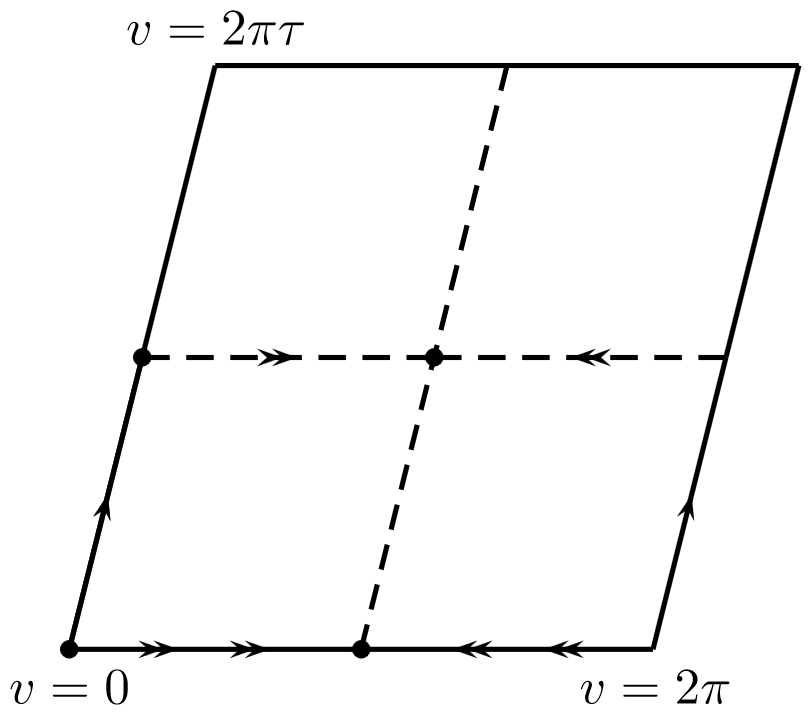
\includegraphics[width=0.85\textwidth]{figures/fig06.png}
  \caption{枕形几何是商 $T^2/\mathbb{Z}_2$。平面上的四点 $0,z,1,\infty$ 分别映到 $\mathbb{Z}_2$ 的不动点 $w=0,\pi,\pi(\tau+1),\pi\tau$。（原文 p.12，图 6）}
  \label{fig:6}
\end{figure}

% [Tutor Note: (3.25) 的 $q=e^{i\pi\tau}$ 是“半周期”nome：枕形的基本周期为 $2\pi$ 与 $2\pi\tau$，故 $q$ 的幂是 $e^{in\pi\tau}$。这与环面配分函数常用的 $q=e^{2\pi i\tau}$ 相差一个因子 2，是抄写 $\theta_3$ 级数时最常见的错误来源。]

从黎曼球上的坐标 $u$ 到枕形上的 $w$ 的显式映射为
\begin{equation}\label{eq:3-26}
  w=\frac{1}{(\theta_3(\tau))^2}\int_0^u\frac{dx}{\sqrt{x(1-x)(z-x)}},
\end{equation}
其中 $\theta_3(\tau)=\sum_{n=-\infty}^{\infty}q^{n^2}$ 是 Jacobi theta 函数之一。在枕形框架中，四个原初算符插入在四个角点 $w=0,\pi,\pi\tau,\pi(1+\tau)$，而共形块可以看作柱面上的传播子~\cite{r11}。

% 原文此处跨页（PDF 第 13 页末）："of as the propagator on the cylinder [11]"，
% 已在上一句收句；ch03b.tex 从 "Its matrix elements are written..." 续译。


% =====================================================================
% ch03b.tex —— 第 3 节后半（PDF p.14–19，原书 p.13–18）
% 译者：tr03b；体例见 work/style_guide.md
% 底本：Xi Yin, Aspects of 2D CFTs, PoS(TASI2017)003
% 说明：本片段从 3.2 节（枕形几何与共形块的解析延拓）的续文开始，
%       故不重复 \subsection 标题；随后依次是 3.3、3.4、3.5 三小节。
% =====================================================================

% 衔接说明：上一段末句“而共形块可以看作柱面上的传播子 [11]”已在 ch03a.tex 收句，
% 本片段从 "Its matrix elements are written..." 续译。
其矩阵元写作
\begin{equation}\label{eq:3-27}
  \langle\psi_{43}|q^{L_0-\frac{c}{24}}|\psi_{12}\rangle
  =\sum_{n=0}^{\infty}a_nq^{h+n-\frac{c}{24}},
\end{equation}
其中 $|\psi_{12}\rangle$ 与 $|\psi_{43}\rangle$ 是一对原初场分别插入枕形几何两个角上时生成的态，并投影到权重为 $h$ 的原初场的 Virasoro 后代表示空间；系数 $a_n$ 依赖权重 $h_i$、$h$ 与中心荷 $c$。\eqref{eq:3-27} 与球面四点共形块只差一个共形反常因子：
\begin{equation}\label{eq:3-28}
  \begin{aligned}
  &\mathcal{F}_c(h_1,h_2,h_3,h_4,h;z)\\
  &\quad=\bigl(\theta_3(\tau)\bigr)^{\frac{c}{2}-4(h_1+h_2+h_3+h_4)}
  \,z^{\frac{c}{24}-h_1-h_2}\,(1-z)^{\frac{c}{24}-h_3-h_4}\,
  \langle\psi_{43}|q^{L_0-\frac{c}{24}}|\psi_{12}\rangle .
  \end{aligned}
\end{equation}

% [Tutor Note: \eqref{eq:3-28} 的指数容易记错：$\theta_3$ 上是 $\frac{c}{2}-4(h_1+h_2+h_3+h_4)$，而 $z$、$1-z$ 上是 $\frac{c}{24}-h_i-h_{i+1}$，两处的 $c$ 系数不同（$\frac{c}{2}$ 与 $\frac{c}{24}$），$h_i$ 的系数也不同（$\theta_3$ 上是 4，$z$ 上是 1）。核对时与 \eqref{eq:3-30} 对照，两式的预因子必须逐字相同。]

共形块的枕形表示 \eqref{eq:3-28} 有几条重要性质。第一，\eqref{eq:3-27} 的 $q$ 展开收敛半径为 1，且在去掉原点的单位 $q$ 圆盘上是全纯函数。这覆盖了整个复 $z$ 平面而有余：复 $z$ 平面其实只映到单位 $q$ 圆盘上的一个眼形区域（图~\ref{fig:7}）。第二，矩阵元 \eqref{eq:3-27} 有性质：若取 $h_1=h_4$、$h_2=h_3$，则系数 $a_n$ 是 $|\psi_{12}\rangle$ 的 Virasoro 后代的模方，因而非负（前提是 OPE 与幺正性相容）。

\begin{figure}[htbp]
  \centering
  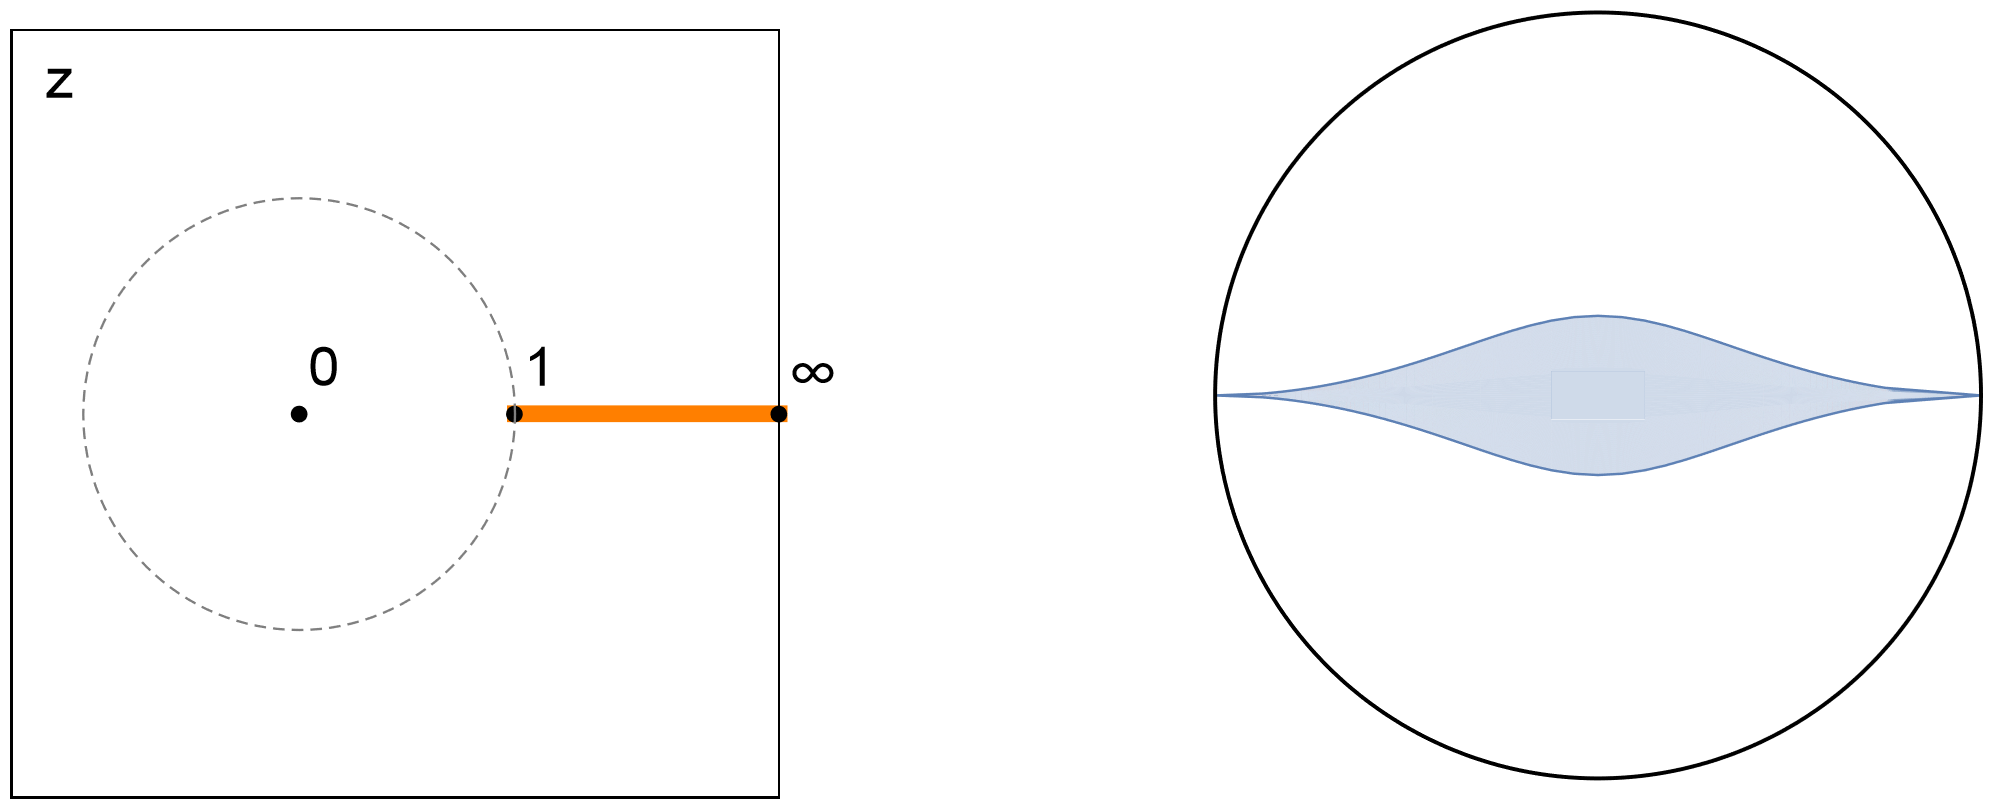
\includegraphics[width=0.85\textwidth]{figures/fig07.png}
  \caption{复 $z$ 平面沿 $[1,\infty)$ 带支割线，映射到单位 $q$ 圆盘上的眼形区域。Virasoro 共形块可解析延拓到整个 $q$ 圆盘。（原文 p.13，图 7）}
  \label{fig:7}
\end{figure}

% [Tutor Note: 图 7 的关键是“映射不覆盖单位 $q$ 圆盘”：$z$ 平面的像只是圆盘内一片眼形区域，两眼尖分别对应 $z=0$ 与 $z=\infty$。正因如此，“$q$ 展开在单位圆盘上收敛”比“$z$ 展开在 $|z|<1$ 收敛”强得多，\eqref{eq:3-28} 才能给出跨过支割线的解析延拓。]

第三，\eqref{eq:3-27} 在 $h\to\infty$ 而 $c$ 与各 $h_i$ 固定的极限下简化：
\begin{equation}\label{eq:3-29}
  \lim_{h\to\infty}\langle\psi_{43}|q^{L_0-\frac{c}{24}}|\psi_{12}\rangle
  =(16q)^{h-\frac{c}{24}}\prod_{n=1}^{\infty}\bigl(1-q^{2n}\bigr)^{-\frac12}.
\end{equation}
从直观上看，大 $h$ 极限下插在角上的外场无关紧要，枕形共形块（至多相差一个与模无关的系数）就等于权重为 $h$ 的原初场环面特征标的平方根。

% [Tutor Note: \eqref{eq:3-29} 里的 $16q$ 是大 $h$ 极限的重标度因子，不能换成 $q$：它来自 $q\to0$ 时 $z=(\theta_2(\tau)/\theta_3(\tau))^4=16q+\cdots$，即 $q$ 与枕形坐标 $z$ 的比值是 16。此式右边的无穷乘积是不含零后代的 Verma 模特征标结构，用来把 \eqref{eq:3-30} 中的 $H_c$ 归一化成 $h\to\infty$ 时趋于 1。]

已知大 $h$ 极限，便可导出以 $h$（而非 $c$）为展开参数的递推公式：
\begin{equation}\label{eq:3-30}
  \begin{aligned}
  \mathcal{F}_c(h_1,h_2,h_3,h_4,h;z)
  &=\bigl(\theta_3(\tau)\bigr)^{\frac{c}{2}-4(h_1+h_2+h_3+h_4)}
  z^{\frac{c}{24}-h_1-h_2}(1-z)^{\frac{c}{24}-h_3-h_4}\\
  &\quad\times(16q)^{h-\frac{c}{24}}
  \prod_{n=1}^{\infty}\bigl(1-q^{2n}\bigr)^{-\frac12}
  H_c(h_1,h_2,h_3,h_4,h;q),
  \end{aligned}
\end{equation}
其中 $H_c$ 满足
\begin{equation}\label{eq:3-31}
  H_c(h_1,h_2,h_3,h_4,h;q)=1+\sum_{r,s\ge1}\frac{q^{rs}}{h-h_{r,s}}\,
  A^c_{rs}P^{rs}_c\begin{bmatrix}h_1\\ h_2\end{bmatrix}
  P^{rs}_c\begin{bmatrix}h_4\\ h_3\end{bmatrix}
  H_c(h_1,h_2,h_3,h_4,h_{r,s}+rs;q).
\end{equation}

% [Tutor Note: \eqref{eq:3-31} 是 Zamolodchikov 的 $h$ 递推（\cite{r10}），与针对 $c$ 的递推 \eqref{eq:3-24} 互为对偶：极点位置由 $c_{r,s}(h)$ 换成 $h_{r,s}(c)$，$A^c_{rs}$ 仍是 \eqref{eq:3-18} 中的量。方括号 $\begin{bmatrix}h_1\\ h_2\end{bmatrix}$ 是对融合矩阵 $P^{rs}_c$ 取相应指标的矩阵元，不是二项式系数。]

实践中可以高效地实现这一递推：先把 \eqref{eq:3-31} 当作线性方程组，对满足 $rs\le n$ 的有限个 $r,s$ 解出 $H_c(h_1,h_2,h_3,h_4,h_{r,s}+rs;q)$ 至 $q^n$ 阶；再用它生成一般内部权重 $h$ 的 $H_c$，同样至 $q^n$ 阶。

\subsection{OPE 的收敛性与交叉方程}

考虑球面四点函数的特例 $\phi_1=\phi_4$、$\phi_2=\phi_3$，它在枕形框架下的共形块分解是求和
\begin{equation}\label{eq:3-32}
  \sum_k C_{12k}^2\,
  \langle\psi^k_{12}|q^{L_0-\frac{c}{24}}|\psi^k_{12}\rangle\,
  \langle\tilde\psi^k_{12}|\bar q^{\bar L_0-\frac{\tilde c}{24}}|\tilde\psi^k_{12}\rangle,
\end{equation}
其中把上标 $k$ 标在 $|\psi^k_{12}\rangle$ 上，用以强调它依赖内部权重 $h_k$。四点函数对 $0<z<1$ 的实 $z$ 解析，故共形块和对 $0<q<1$ 的实 $q$ 收敛；又因 \eqref{eq:3-27} 的系数 $a_n$ 非负，由 Cauchy--Schwarz 不等式即知它对整个 $q$ 圆盘收敛。\eqref{eq:3-32} 的被加项在大内部权重极限下按 $C_{12k}^2(16q)^{h_k+\tilde h_k}$ 增长，于是实 $q$ 接近 1 时的收敛性表明：在单位 $q$ 圆盘内部、$h_*,\tilde h_*\to\infty$ 的极限下，权重 $h_k>h_*$、$\tilde h_k>\tilde h_*$ 的算符对 \eqref{eq:3-32} 的贡献被 $|q|^{h_*+\tilde h_*}$ 压低（若把 $h_k$ 或 $\tilde h_k$ 之一保持在有限区间，可作类似论证）。这一结果说明：枕形框架下 $\phi_1\phi_2$ 的 OPE 作为对内部原初场的求和，以指数式快的速度收敛。

% [Tutor Note: 由实 $q$ 的收敛推出整个 $q$ 圆盘上的收敛，靠的正是 $a_n\ge0$：此时 \eqref{eq:3-27} 呈平方和结构，Cauchy--Schwarz 不等式给出 $q$ 圆盘边界上的收敛性，再作解析延拓。另，原文此处的 “convergences” 应为 “converges”，属语法笔误，不影响数学内容。]

理解共形块展开的收敛性之后，便可把一个一般四点函数 $\langle\prod_{i=1}^4\phi_i(z_i,\bar z_i)\rangle$ 按三种不同通道分解：
\begin{equation}\label{eq:3-33}
  s:\,12\to34,\qquad t:\,14\to23,\qquad u:\,13\to24 .
\end{equation}

% [Tutor Note: \eqref{eq:3-33} 的箭头读作“先对箭头左侧两场作 OPE，再与右侧两场缩并”，即 $s$ 通道配对 $(\phi_1\phi_2)(\phi_3\phi_4)$，$t$ 通道配对 $(\phi_1\phi_4)(\phi_2\phi_3)$。原文只写配对编号，省略了箭头的含义。]

这些共形块分解的等价性给结构常数很强的约束。在外场的各种置换意义下，只需检查 $s$ 通道与 $t$ 通道的等价。把 $z\to1-z$ 并同时交换 $h_1$ 与 $h_3$，便从 $s$ 通道共形块得到 $t$ 通道共形块。两者的等价可写成交叉方程
\begin{equation}\label{eq:3-34}
  \begin{aligned}
  &\sum_k C_{12k}C_{34k}\,
  \mathcal{F}_c(h_1,h_2,h_3,h_4,h_k;z)\,
  \overline{\mathcal{F}}_c(\tilde h_1,\tilde h_2,\tilde h_3,\tilde h_4,\tilde h_k;\bar z)\\
  &\quad=\sum_k C_{14k}C_{23k}\,
  \mathcal{F}_c(h_3,h_2,h_1,h_4,h_k;1-z)\,
  \overline{\mathcal{F}}_c(\tilde h_3,\tilde h_2,\tilde h_1,\tilde h_4,\tilde h_k;1-\bar z).
  \end{aligned}
\end{equation}

% [Tutor Note: \eqref{eq:3-34} 就是二维修正自举的出发点。注意右边第一个共形块的宗量顺序是 $(h_3,h_2,h_1,h_4)$ 而非 $(h_1,h_3,\dots)$：$t$ 通道把 1 与 3 交换，故 1、3 两个位置上的权重随之交换，但 2、4 的位置不动。]

\subsection{交叉方程的解：极小模型}

现在讨论交叉方程最简单的非平凡解之一：$c=\frac12$ 极小模型中非平凡原初场的四点函数。这个模型又称二维临界 Ising 模型。该 CFT 只有三个原初场，权重为
\begin{equation}\label{eq:3-35}
  \begin{aligned}
  1&:\quad h=\tilde h=h_{1,1}=0,\\
  \sigma&:\quad h=\tilde h=h_{1,2}=\frac{1}{16},\\
  \varepsilon&:\quad h=\tilde h=h_{2,1}=\frac12 .
  \end{aligned}
\end{equation}

我们聚焦四点函数 $\langle\sigma(0)\sigma(z,\bar z)\sigma(1)\sigma'(\infty)\rangle\equiv f(z,\bar z)$ 这一例子。$\sigma$ 在能级 2 有一个零后代，形如
\begin{equation}\label{eq:3-36}
  \Bigl(L_{-1}^2-\frac34L_{-2}\Bigr)\sigma
  =\Bigl(\bar L_{-1}^2-\frac34\bar L_{-2}\Bigr)\sigma=0 .
\end{equation}

% [Tutor Note: \eqref{eq:3-36} 的系数 $\frac34$ 来自一般的能级 2 零矢量 $\bigl(L_{-1}^2-\frac{2(2h+1)}{3}L_{-2}\bigr)|h\rangle=0$；代入 $h=h_{1,2}=\frac{1}{16}$ 得 $\frac{2(2h+1)}{3}=\frac34$。这类零矢量沿退化曲线 $h=h_{1,2}(c)$（以及 $h=h_{2,1}(c)$）都存在，$c=\frac12$、$h=\frac{1}{16}$ 只是其中的 Ising 点；正是这类零态使极小模型的共形块可解。]

把 \eqref{eq:3-36} 代入四点函数，得
\begin{equation}\label{eq:3-37}
  \Bigl\langle\sigma(0)\Bigl(L_{-1}^2-\frac34L_{-2}\Bigr)\sigma(z,\bar z)\sigma(1)\sigma'(\infty)\Bigr\rangle=0 .
\end{equation}

作用在 $\sigma(z)$ 上的 $L_{-1}$ 可替换为 $\partial_z$。涉及 $L_{-2}\sigma(z,\bar z)$ 的关联函数用下式计算：
\begin{equation}\label{eq:3-38}
  \begin{aligned}
  &\langle\sigma|\sigma(1)L_{-2}\sigma(z,\bar z)|\sigma\rangle
  =\oint_{C_z}\frac{dw}{2\pi i}\,\frac{1}{w-z}\,
  \langle\sigma|\sigma(1)T(w)\sigma(z)|\sigma\rangle\\
  &\quad=h_{1,2}\Bigl[\frac{1}{(1-z)^2}+\frac{1}{z^2}\Bigr]
  \langle\sigma|\sigma(1)\sigma(z,\bar z)|\sigma\rangle
  -\frac{1}{1-z}\langle\sigma|\partial\sigma(1)\sigma(z,\bar z)|\sigma\rangle
  +\frac1z\langle\sigma|\sigma(1)\sigma(z,\bar z)|\partial\sigma\rangle .
  \end{aligned}
\end{equation}

% [Tutor Note: \eqref{eq:3-38} 第二行的三项分别来自 $T(w)$ 与 $\sigma(1)$、$\sigma(0)$ 的 OPE：$h$ 项给出 $1/(1-z)^2+1/z^2$ 两个双极点，$\partial\sigma(1)$ 与 $\partial\sigma(0)$ 项给出 $-\frac{1}{1-z}$ 与 $+\frac1z$ 两个单极点。末项的 ket $|\partial\sigma\rangle$ 是 $\partial\sigma(0)|0\rangle$ 的简写。核对时注意围道的取向：取向反了会让两个单极点的符号同时翻转。]

涉及 $\partial\sigma$ 的关联函数，可以回到由 $PSL(2,\mathbb{C})$ 不变性确定的一般四点函数形式来计算：
\begin{equation}\label{eq:3-39}
  \langle\sigma(z_1,\bar z_1)\sigma(z_2,\bar z_2)\sigma(z_3,\bar z_3)\sigma'(\infty)\rangle
  =\frac{1}{|z_{31}|^{4h_{1,2}}}\,
  f\Bigl(\frac{z_{21}}{z_{31}},\frac{\bar z_{21}}{\bar z_{31}}\Bigr),
\end{equation}
于是
\begin{equation}\label{eq:3-40}
  \begin{aligned}
  \langle\sigma(0)\sigma(z,\bar z)\partial\sigma(1)\sigma'(\infty)\rangle
  &=\partial_{z_3}\frac{1}{|z_{31}|^{4h_{1,2}}}
  f\Bigl(\frac{z_{21}}{z_{31}},\frac{\bar z_{21}}{\bar z_{31}}\Bigr)
  \Big|_{\substack{z_1=0,\,z_2=z\\ z_3=1}}
  =(-z\partial_z-2h_{1,2})f(z,\bar z),\\
  \langle\partial\sigma(0)\sigma(z,\bar z)\sigma(1)\sigma'(\infty)\rangle
  &=\partial_{z_1}\frac{1}{|z_{31}|^{4h_{1,2}}}
  f\Bigl(\frac{z_{21}}{z_{31}},\frac{\bar z_{21}}{\bar z_{31}}\Bigr)
  \Big|_{\substack{z_1=0,\,z_2=z\\ z_3=1}}
  =\bigl((z-1)\partial_z+2h_{1,2}\bigr)f(z,\bar z).
  \end{aligned}
\end{equation}

% [Tutor Note: 核对 \eqref{eq:3-40} 时用链式法则：全纯部分 $\partial_{z_3}(z_{31})^{-2h_{1,2}}=-2h_{1,2}(z_{31})^{-2h_{1,2}-1}$ 在 $z_3=1$ 处给 $-2h_{1,2}$，而 $\partial_{z_3}(z_{21}/z_{31})=-z$；类似地 $\partial_{z_1}(z_{21}/z_{31})=z-1$、$\partial_{z_1}(z_{31})^{-2h_{1,2}}=2h_{1,2}$。两式合起来把 \eqref{eq:3-38} 中的 $\partial\sigma$ 与 $\partial_z$ 项化到同一个 $f$ 上，再代入 \eqref{eq:3-37} 即得 \eqref{eq:3-41}。]

把 \eqref{eq:3-38} 与 \eqref{eq:3-40} 代入 \eqref{eq:3-37}，得到
\begin{equation}\label{eq:3-41}
  \Bigl[\partial_z^2+\frac{3(1-2z)}{4z(1-z)}\partial_z
  -\frac{3}{64z^2(1-z)^2}\Bigr]f(z,\bar z)=0 .
\end{equation}
此方程有两个线性无关解：
\begin{equation}\label{eq:3-42}
  f_\pm(z)=\frac{\sqrt{1\pm\sqrt z}}{z^{\frac18}(1-z)^{\frac18}} .
\end{equation}

这两个解的线性组合给出两种可能的共形块。此例中只有有限个（即两个）共形块，这是 $\sigma$ 存在零 Virasoro 后代造成的偶然现象。在 $z=0$ 附近展开，得
\begin{equation}\label{eq:3-43}
  \begin{aligned}
  \mathcal{F}_0(z)&=\frac{f_+(z)+f_-(z)}{2}
  =z^{-\frac18}\Bigl(1+\frac{1}{64}z^2+\frac{1}{64}z^3+\frac{117}{8192}z^4+\cdots\Bigr),\\
  \mathcal{F}_{\frac12}(z)&=f_+(z)-f_-(z)
  =z^{\frac38}\Bigl(1+\frac14z+\frac{9}{64}z^2+\frac{25}{256}z^3+\frac{613}{8192}z^4+\cdots\Bigr).
  \end{aligned}
\end{equation}

% [Tutor Note: 展开式的首项指数给出内部权重，$\mathcal{F}_h(z)\sim z^{h-2h_\sigma}$；这里 $2h_\sigma=\frac18$，故 $h=0$ 给 $z^{-1/8}$、$h=\frac12$ 给 $z^{3/8}$，两者指数差 $\frac12=h_\varepsilon$。另，$\mathcal{F}_0$ 展开中 $z^2$ 与 $z^3$ 的系数同为 $\frac{1}{64}$ 并非笔误：$z$ 的一次项在 $f_++f_-$ 中恰好抵消，而 $z^2$、$z^3$ 两项的系数确实相等。]

如记号所示，$\mathcal{F}_h(z)$ 是 $\langle\sigma\sigma\sigma\sigma\rangle$ 中内部原初场权重为 $h$ 的共形块。这里只有单位算符与 $\varepsilon$ 能出现在 $\sigma\sigma$ OPE 中，这是零态微分方程的结果。四点函数因而必取形式
\begin{equation}\label{eq:3-44}
  f(z,\bar z)=\mathcal{F}_0(z)\overline{\mathcal{F}}_0(\bar z)
  +C_{\sigma\sigma\varepsilon}^2\,\mathcal{F}_{\frac12}(z)
  \overline{\mathcal{F}}_{\frac12}(\bar z).
\end{equation}

现在检查交叉对称性：它要求 $f(z,\bar z)$ 在 $z\to1-z$、$\bar z\to1-\bar z$ 下不变。取支割线从 $z=1$ 延伸到 $\infty$，$f_\pm(z)$ 满足
\begin{equation}\label{eq:3-45}
  f_+(1-z)=\frac{f_+(z)+f_-(z)}{\sqrt2},\qquad
  f_-(1-z)=\frac{f_+(z)-f_-(z)}{\sqrt2} .
\end{equation}

% [Tutor Note: \eqref{eq:3-45} 是 $z\to1-z$ 的“单值性字典”，它把绕支点的解析延拓写成两个解之间的正交变换。用它可以把 $\mathcal{F}_0(1-z)$、$\mathcal{F}_{1/2}(1-z)$ 反解成 $\mathcal{F}_0(z)$、$\mathcal{F}_{1/2}(z)$ 的组合：由 $f_\pm=\mathcal{F}_0\pm\frac12\mathcal{F}_{1/2}$ 可得 $\mathcal{F}_0(1-z)=\frac{1}{\sqrt2}\mathcal{F}_0+\frac{1}{2\sqrt2}\mathcal{F}_{1/2}$、$\mathcal{F}_{1/2}(1-z)=\sqrt2\,\mathcal{F}_0-\frac{1}{\sqrt2}\mathcal{F}_{1/2}$。]

于是有
\begin{equation}\label{eq:3-46}
  f(1-z,1-\bar z)
  =\Bigl|\frac{1}{\sqrt2}\mathcal{F}_0+\frac{1}{2\sqrt2}\mathcal{F}_{\frac12}\Bigr|^2
  +C_{\sigma\sigma\varepsilon}^2
  \Bigl|\sqrt2\,\mathcal{F}_0-\frac{1}{\sqrt2}\mathcal{F}_{\frac12}\Bigr|^2 .
\end{equation}

% [Tutor Note: 把 \eqref{eq:3-46} 与 \eqref{eq:3-44} 逐项比较即可定出 $C$：$\mathcal{F}_0\bar{\mathcal{F}}_{1/2}$ 的系数给出 $\frac12-2C^2=0$，即 $C^2=\frac14$；$\mathcal{F}_0\bar{\mathcal{F}}_0$ 与 $\mathcal{F}_{1/2}\bar{\mathcal{F}}_{1/2}$ 的系数给出同一条件。可见交叉对称性把 $C$ 唯一确定为 $\frac12$（符号取正由幺正性）。]

可见交叉对称性成立当且仅当
\begin{equation}\label{eq:3-47}
  C_{\sigma\sigma\varepsilon}=\frac12 .
\end{equation}

事实上，$C_{\sigma\sigma\varepsilon}$ 是 $c=\frac12$ 极小模型中唯一的非平凡结构常数：用类似的分析可证 $C_{\varepsilon\varepsilon\sigma}$ 与 $C_{\varepsilon\varepsilon\varepsilon}$ 都为零。该 CFT 由此完全解出。

还有一组一致性条件必须满足，即原初场环面一点函数的模协变性。它对 $c=\frac12$ 极小模型确实成立，但此处不作显式验证。

% [Tutor Note: 这里说的“模协变性”指环面一点函数在 $SL(2,\mathbb{Z})$ 下的变换性质；极小模型的各原初场都对应已知的模不变配分函数组合，故该条件是自动的。作者略去验证，是因为它不影响球面四点函数的解。]

\subsection{交叉方程的解：Liouville 理论}

现在描述交叉方程的另一个非平凡解。考虑中心荷 $c>1$ 的幺正 CFT，并假设其中只有标量 Virasoro 原初场。假设 $c>1$，是为了让零的 Virasoro 后代不可能出现。要求所有 Virasoro 原初场都是标量，即 $h=\tilde h$，是极强的条件；事实上，这一条件（在猜想意义上）完全固定了该 CFT！

先考察这种 CFT 的环面配分函数，它必须模不变。其一般形式为
\begin{equation}\label{eq:3-48}
  Z(\tau,\bar\tau)=\sum_{h,\tilde h}d_{h,\tilde h}\,
  \chi_h(\tau)\bar\chi_{\tilde h}(\bar\tau),
\end{equation}
其中 $d_{h,\tilde h}$ 是权重为 $(h,\tilde h)$ 的原初场个数，$\chi_h$ 是权重为 $h$ 的原初场的 Virasoro 表示的环面特征标，
\begin{equation}\label{eq:3-49}
  \chi_h(\tau)=\mathrm{Tr}_{\mathcal{V}_h}\,q^{h-\frac{c}{24}},
\end{equation}
其中 $q=e^{2\pi i\tau}$，$\mathcal{V}_h$ 是 $v_h$ 的 Virasoro 后代构成的空间。没有零后代时（$c>1$ 且 $h\ge0$ 保证这一点），有
\begin{equation}\label{eq:3-50}
  \chi_h(\tau)=q^{h-\frac{c}{24}}\prod_{n=1}^{\infty}\frac{1}{1-q^n}.
\end{equation}

% [Tutor Note: \eqref{eq:3-49} 的迹是 $L_0-\frac{c}{24}$ 的指数；\eqref{eq:3-50} 中每个因子 $1/(1-q^n)$ 对应 $L_{-n}$ 取任意次幂。若 $c\le1$ 或 $h<0$，Verma 模含零后代，必须逐个扣除，此式不再成立。还要注意约定：本小节（环面）用 $q=e^{2\pi i\tau}$，而上一小节枕形框架用 $q=e^{i\pi\tau}$，两处的 $q$ 不能混用。]

暂时设 $\tilde c=c$，于是反全纯 Virasoro 特征标就是 $\chi_{\tilde h}$ 的复共轭。模不变性等价于
\begin{equation}\label{eq:3-51}
  Z(\tau,\bar\tau)=Z(\tau+1,\bar\tau+1)=Z(-1/\tau,-1/\bar\tau).
\end{equation}

第一个等式等价于对所有原初场 $h-\tilde h\in\mathbb{Z}$，即自旋为整数。若只有标量原初场（$h=\tilde h$），这一点自然满足。对第二个等式，把配分函数写成
\begin{equation}\label{eq:3-52}
  Z(\tau,\bar\tau)=\frac{1}{|\eta(\tau)|^2}
  \sum_h d_h\exp\Bigl[-4\pi\tau_2\Bigl(h-\frac{c-1}{24}\Bigr)\Bigr],
\end{equation}
再利用 $\eta$ 函数的模性质 $\eta(-1/\tau)=\sqrt{-i\tau}\,\eta(\tau)$，配分函数的模不变性便可写成
\begin{equation}\label{eq:3-53}
  \frac{1}{|\tau|}\sum_h d_h
  \exp\Bigl[-4\pi\frac{\tau_2}{|\tau|^2}\Bigl(h-\frac{c-1}{24}\Bigr)\Bigr]
  =\sum_h d_h\exp\Bigl[-4\pi\tau_2\Bigl(h-\frac{c-1}{24}\Bigr)\Bigr].
\end{equation}

% [Tutor Note: \eqref{eq:3-52} 的 $c-1$ 是这样来的：由 $\eta(\tau)=q^{1/24}\prod(1-q^n)$ 得 $\prod_n(1-q^n)^{-1}=q^{-1/24}/\eta$，故 $\chi_h=q^{h-c/24}\prod(1-q^n)^{-1}=q^{h-(c-1)/24}/\eta$，指数里便出现 $h-\frac{c-1}{24}$，而不是 $h-\frac{c}{24}$。又在取模方时 $|q^{h-(c-1)/24}|^2=e^{-4\pi\tau_2(h-(c-1)/24)}$，其中用到 $\tau_2=\mathrm{Im}\,\tau$。]

为看得更清楚，定义
\begin{equation}\label{eq:3-54}
  x=\tau_2,\qquad y=\frac{\tau_2}{|\tau|^2},
\end{equation}
并把上式写成
\begin{equation}\label{eq:3-55}
  \sqrt{y}\sum_h d_h\exp\Bigl[-4\pi y\Bigl(h-\frac{c-1}{24}\Bigr)\Bigr]
  =\sqrt{x}\sum_h d_h\exp\Bigl[-4\pi x\Bigl(h-\frac{c-1}{24}\Bigr)\Bigr].
\end{equation}

% [Tutor Note: 由 $y=\tau_2/|\tau|^2$ 与 $x=\tau_2$ 得 $|\tau|^2=x/y$，故 $\frac{1}{|\tau|}=\sqrt{y/x}$；\eqref{eq:3-53} 两边同乘 $|\tau|=\sqrt{x/y}$ 即得 \eqref{eq:3-55}，这一步只是变量替换，没有额外假设。]

显然，这只有在两边都与 $x$、$y$ 无关时才可能，即
\begin{equation}\label{eq:3-56}
  \sum_h d_h\exp\Bigl[-4\pi x\Bigl(h-\frac{c-1}{24}\Bigr)\Bigr]\propto x^{-\frac12}.
\end{equation}

对离散的原初场谱，这实际上不可能。我们需要的是权重 $h\ge\frac{c-1}{24}$ 的一族连续原初场，并把求和换成带谱密度 $\rho(h)$ 的积分：
\begin{equation}\label{eq:3-57}
  \sum_h d_h\to\int_{\frac{c-1}{24}}^{\infty}dh\,\rho(h),
\end{equation}
其中
\begin{equation}\label{eq:3-58}
  \rho(h)\propto\frac{1}{\sqrt{h-\frac{c-1}{24}}}.
\end{equation}

% [Tutor Note: 从 \eqref{eq:3-56} 到 \eqref{eq:3-58} 用的是 Laplace 变换：若 $\int_{h_0}^{\infty}dh\,\rho(h)e^{-4\pi x(h-h_0)}\propto x^{-1/2}$，由 $\int_0^{\infty}dt\,t^{-1/2}e^{-4\pi xt}=\Gamma(\frac12)(4\pi x)^{-1/2}$ 即知 $\rho(h)\propto(h-h_0)^{-1/2}$，$h_0=\frac{c-1}{24}$。离散谱之所以不行，是因为有限项指数和在大 $x$ 时按 $e^{-4\pi x\,\Delta}$ 衰减，不可能给出幂律 $x^{-1/2}$。]

若写 $c=1+6Q^2$、$h=\frac{Q^2}{4}+P^2$，则
\begin{equation}\label{eq:3-59}
  \int_{\frac{c-1}{24}}^{\infty}dh\,\rho(h)\propto\int_0^{\infty}dP .
\end{equation}
由此可知，原初场的谱密度对参数 $P$ 必须是平坦分布。

% [Tutor Note: \eqref{eq:3-59} 的下限 $\frac{c-1}{24}=\frac{6Q^2}{24}=\frac{Q^2}{4}$ 正是 $h=\frac{Q^2}{4}+P^2$ 在 $P=0$ 处的值；又 $dh=2P\,dP$，而 \eqref{eq:3-58} 给 $\rho\propto(h-\frac{Q^2}{4})^{-1/2}=1/P$，两者相乘恰好给出平坦的 $dP$ 测度，这就是 \eqref{eq:3-59} 的来历。]

假设没有更多简并，于是标量原初场由 $P$ 标记，记作 $V_P$。两点函数自然归一化为
\begin{equation}\label{eq:3-60}
  \langle V_P(1)V_{P'}(0)\rangle=\delta(P-P').
\end{equation}
结构常数现在是三变量的对称函数 $C(P_1,P_2,P_3)$，OPE 取形式
\begin{equation}\label{eq:3-61}
  V_{P_1}(z,\bar z)V_{P_2}(0)\sim\int_0^{\infty}dP_3\,
  C(P_1,P_2,P_3)\,|z|^{-\frac{Q^2}{2}-2P_1^2-2P_2^2+2P_3^2}
  V_{P_3}(0),
\end{equation}
再加上 Virasoro 后代的贡献。

% [Tutor Note: \eqref{eq:3-61} 的指数可用 $\Delta_i=\frac{Q^2}{4}+P_i^2$ 核对：OPE 系数应为 $|z|^{2(\Delta_3-\Delta_1-\Delta_2)}=|z|^{-Q^2/2-2P_1^2-2P_2^2+2P_3^2}$，注意先算 $2(\Delta_3-\Delta_1-\Delta_2)$，容易漏掉 $Q^2$ 项。]

就球面关联函数而言，关键的一致性条件是交叉方程
\begin{equation}\label{eq:3-62}
  \begin{aligned}
  &\int_0^{\infty}dP\,C(P_1,P_2,P)C(P_3,P_4,P)
  \Bigl|\mathcal{F}_c\Bigl(h_1,h_2,h_3,h_4,h=\frac{Q^2}{4}+P^2;z\Bigr)\Bigr|^2\\
  &\quad=\int_0^{\infty}dP\,C(P_3,P_2,P)C(P_1,P_4,P)
  \Bigl|\mathcal{F}_c\Bigl(h_3,h_2,h_1,h_4,h=\frac{Q^2}{4}+P^2;1-z\Bigr)\Bigr|^2 .
  \end{aligned}
\end{equation}

% [Tutor Note: 与 \eqref{eq:3-34} 相比，连续谱的交叉方程把对 $k$ 的求和换成 $\int_0^{\infty}dP$，并对每个共形块取模方：左右两侧共用同一个内部参数 $P$，不是把两个不同 $P$ 的块相乘。权重 $\frac{Q^2}{4}+P^2$ 对 $P$ 与 $-P$ 相同，故积分只取 $P\ge0$。]

是否存在实值函数 $C(P_1,P_2,P_3)$，使该方程对一切 $P_i$ 都成立？值得注意的是，答案是肯定的，而且解看起来唯一（至多相差一个整体常数倍）。该解称为 Dorn--Otto--Zamolodchikov--Zamolodchikov（DOZZ）结构常数，由下式给出 \cite{r12,r13,r14,r15}：
\begin{equation}\label{eq:3-63}
  C(P_1,P_2,P_3)
  =\frac{\Upsilon_b'(0)}{\Upsilon_b\bigl(\frac{Q}{2}+i(P_1+P_2+P_3)\bigr)}
  \prod_{j=1}^{3}
  \frac{\sqrt{\Upsilon_b(2iP_j)\Upsilon_b(-2iP_j)}}
  {\Upsilon_b\bigl(\frac{Q}{2}+i(P_1+P_2+P_3-2P_j)\bigr)},
\end{equation}
其中 $\Upsilon_b(x)$ 是 Barnes 双重 Gamma 函数，定义为下式从区域 $0<\mathrm{Re}(x)<Q$ 出发的解析延拓：
\begin{equation}\label{eq:3-64}
  \Upsilon_b(x)=\exp\Biggl\{
  \int_0^{\infty}\frac{dt}{t}
  \Biggl[\Bigl(\frac{Q}{2}-x\Bigr)^2e^{-t}
  -\frac{\sinh^2\bigl[\bigl(\frac{Q}{2}-x\bigr)\frac{t}{2}\bigr]}
  {\sinh\frac{tb}{2}\,\sinh\frac{t}{2b}}\Biggr]\Biggr\}.
\end{equation}

% [Tutor Note: \eqref{eq:3-63} 分子里 $\sqrt{\Upsilon_b(2iP_j)\Upsilon_b(-2iP_j)}$ 的写法与多数文献的 DOZZ 形式（分子直接写 $\Upsilon_b(2\alpha_j)$，$\alpha_j=\frac{Q}{2}+iP_j$）不同；由 \eqref{eq:3-65} 的反射关系有 $\Upsilon_b(2\alpha_j)=\Upsilon_b(Q+2iP_j)=\Upsilon_b(-2iP_j)$。两种写法至多相差一个由 $\Upsilon_b(2iP_j)$ 决定的因子，引用别的归一化时务必核对。]

% [Tutor Note: \eqref{eq:3-64} 的积分表示有收敛域限制：$t\to\infty$ 时 $\sinh^2$ 之比趋于 $e^{-xt}$，被积函数按 $e^{-xt}$ 衰减；$t\to0$ 时方括号内两项的领头阶相互抵消，积分才在原点附近有限。作者先在 $0<\mathrm{Re}(x)<Q$ 内定义它，再解析延拓成整函数。]

对一般的 $b$，$\Upsilon_b(x)$ 是复 $x$ 平面上的整解析函数，其单零点位于 $x=mb+n/b$，其中整数 $m,n\le0$ 或 $m,n\ge1$。另外几条有用的性质是
\begin{equation}\label{eq:3-65}
  \begin{aligned}
  \Upsilon_b(Q-x)&=\Upsilon_b(x),\\
  \Upsilon_b(x+b)&=\gamma(bx)\,b^{1-2bx}\,\Upsilon_b(x),\\
  \Upsilon_b(x+b^{-1})&=\gamma(b^{-1}x)\,b^{\frac{2x}{b}-1}\,\Upsilon_b(x),
  \end{aligned}
\end{equation}
其中 $\gamma(x)\equiv\Gamma(x)/\Gamma(1-x)$。

% [Tutor Note: \eqref{eq:3-65} 的三行分别给出关于 $Q/2$ 的对称性与沿 $b$、$1/b$ 两个方向的平移规律；零点位置 $x=mb+n/b$（$m,n\le0$ 或 $m,n\ge1$）正是 \eqref{eq:3-63} 分母中 $\Upsilon_b$ 的零点所在，因此 DOZZ 结构常数只在融合规则允许的取值处出现奇点。]

事实表明，取这组结构常数时，环面一点函数的模协变性也得到满足 \cite{r16}。只含标量原初场的谱连同 DOZZ 结构常数，定义的就是所谓的 Liouville CFT \cite{r15,r17}。



% ============================================================
% chapters/ch04a.tex
% Xi Yin, "Aspects of Two-Dimensional Conformal Field Theories"
% PoS(TASI2017)003 · 第 4 章上半（PDF 第 20–26 页，原书 p.19–25）
% 译者：tr04a
% 说明：原文 [N] 一律转写为对应的 \cite{rN}；公式编号与原书一致（eq:3-66…eq:3-69, eq:4-1…eq:4-27）。
% ============================================================
%
% ------------------------------------------------------------------
% 注：下面两段文字与原式 (3.66)–(3.69)、图 8 位于 PDF 第 20 页上半，
% 在原文中属于第 3 节（Liouville CFT）的结尾。ch03b 的页码范围止于原书 p.18，
% 为免两章之间出现断页缺口，此处先行译出；拼接时可由编辑决定归属。
% ------------------------------------------------------------------

Liouville CFT 也可以用更常规的方式定义，例如正则量子化，出发点是经典作用量
\begin{equation}
  \label{eq:3-66}
  S_L=\frac{1}{4\pi}\int d^2z\,\sqrt{g}\left(g^{mn}\partial_m\phi\partial_n\phi+QR\phi+4\pi\mu e^{2b\phi}\right),
\end{equation}
其中 $\mu$ 为任意正常数。在柱面上，可以把 $\phi(\sigma,\tau)$ 按傅里叶模式展开，
\begin{equation}
  \label{eq:3-67}
  \phi(\sigma,\tau)=\sum_{n=-\infty}^{\infty}\phi_n(\tau)e^{in\sigma}.
\end{equation}

\begin{figure}[htbp]
  \centering
  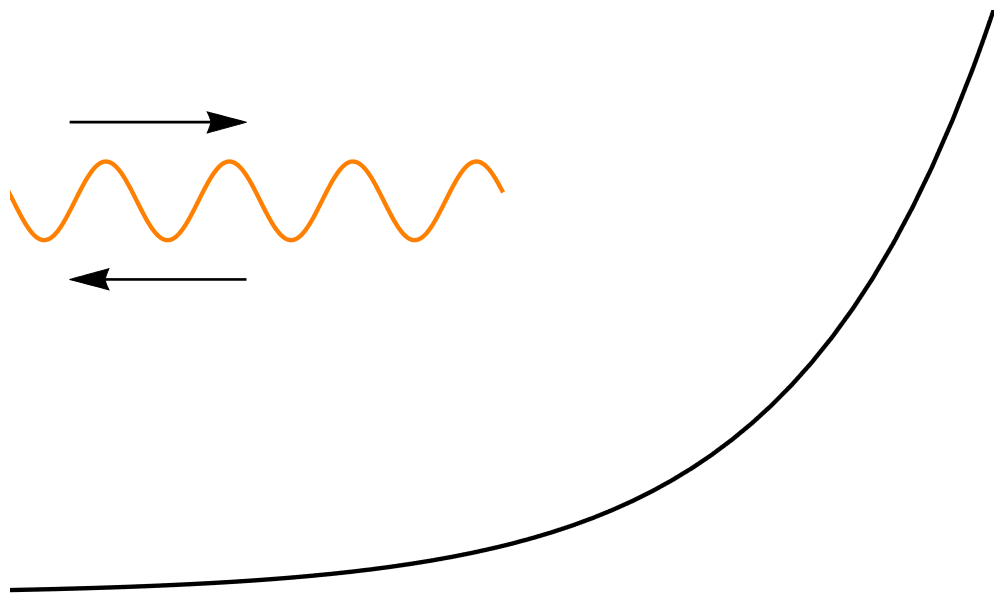
\includegraphics[width=0.85\textwidth]{figures/fig08.png}
  \caption{Liouville CFT 中的标量原初场描述场空间中偏离 Liouville 墙的散射态。（原文 p.19，图 8）}
  \label{fig:8}
\end{figure}

特别地，零模 $\phi_0(\tau)$ 受到势 $V(\phi_0)=2\pi\mu e^{2b\phi_0}$ 的作用。若忽略 $n\neq0$ 的振子 $\phi_n$——在 $\phi_0\to-\infty$ 区域，对最低激发态而言这个近似可以成立——则能量本征态是由如下渐近波函数描述的散射态
\begin{equation}
  \label{eq:3-68}
  \Psi_P(\phi_0)\sim S(P)^{-\frac{1}{2}}e^{2iP\phi_0}+S(P)^{\frac{1}{2}}e^{-2iP\phi_0},
\end{equation}
其能量为
\begin{equation}
  \label{eq:3-69}
  h+\tilde h-\frac{c}{12}=2P^2.
\end{equation}
这些就是柱面上对应原初场 $V_P$ 的态。
% [Tutor Note: 按 p.18 的约定 $c=1+6Q^2$、$h=\frac{Q^2}{4}+P^2$ 直接代入，应有 $h+\tilde h-\frac{c}{12}=2P^2-\frac{1}{12}$；原文 (3.69) 少了 $-\frac{1}{12}$，也可能是作者把柱面能量零点另行约定，引用此式时须核对。]

\section{已知二维 CFT 概览}\label{sec:4}

\begin{keytakeaways}
  \item 核心物理图像：二维 CFT 有几类基本构造——自由玻色子的手征与反手征分量、离散对称群的轨形、流代数的 WZW 模型与陪集，以及非线性 sigma 模型。它们共同的约束是 OPE 的单值性与结合性、幺正性，以及环面上的模不变性。
  \item 使用的数学工具：偶自对偶格（Narain 格）、共轭类与扭曲扇区、拓扑线算符、仿射李代数及其 Sugawara 构造、顶点算符代数与模矩阵 $S,T$、$\beta$ 函数与 Ricci 流。
  \item 本节结论：模不变性把 Narain 格的动量格限制为偶自对偶格；轨形的扭曲扇区谱由扭曲环面配分函数 $Z^g_h$ 决定；WZW 模型的中心荷为 $c^G=k\dim G/(k+h)$；RCFT 的谱只含有限多个表示且 $S^2=(ST)^3=\mathbb{I}$，故中心荷必为有理数；NLSM 的共形不变性等价于 $\beta^G_{ij}=\beta^\Phi=0$，即靶空间度规满足运动方程。
\end{keytakeaways}

下面我们简要回顾二维中一些已知的幺正 CFT 的构造。

\subsection{Narain 格}\label{sec:4-1}

一族基本的 CFT 由自由玻色子的全纯分量与反全纯分量构造，它们可由如下 OPE 定义：
\begin{equation}
  \label{eq:4-1}
  X_L^i(z)X_L^j(0)\sim-\delta^{ij}\ln z,\qquad X_R^i(\bar z)X_R^j(0)\sim-\delta^{ij}\ln\bar z .
\end{equation}
当然，这些场并非单值；思路是用它们构造出满足单值、结合 OPE 的算符，并且要求算符谱同时模不变。

% [Tutor Note: (4.1) 的系数 $-\delta^{ij}$ 与两点函数 $\langle X(z)X(0)\rangle=-\ln|z|^2$ 的约定一致。若采用带 $\alpha'$ 的约定 $X^iX^j\sim-\frac{\alpha'}{2}\delta^{ij}\ln z$，则 (4.3) 的顶点算符要相应乘 $\sqrt{2/\alpha'}$，(4.4) 的整内积条件也会随之改动；比较不同文献时须先确认此项归一化。]

我们先取一组 $U(1)^{n_L}$ 全纯流与 $U(1)^{n_R}$ 反全纯流，
\begin{equation}
  \label{eq:4-2}
  j^i(z)=\partial X_L^i(z),\qquad \tilde j^i(\bar z)=\bar\partial X_R^i(\bar z).
\end{equation}

接下来考虑如下形式的流代数原初场
\begin{equation}
  \label{eq:4-3}
  V_{k_L,k_R}=\,:e^{ik_L\cdot X_L+ik_R\cdot X_R}:,
\end{equation}
其中 $k=(k_L,k_R)$ 视为 $\mathbb{R}^{n,m}$ 中的矢量。OPE 的自洽性要求 $k$ 取值于一个内积为整数的格 $\Gamma\subset\mathbb{R}^{n,m}$：
\begin{equation}
  \label{eq:4-4}
  k\circ k'\equiv k_L\cdot k'_L-k_R\cdot k'_R\in\mathbb{Z}.
\end{equation}
模不变性进一步要求 $\Gamma$ 是偶格且自对偶 \cite{r18}。设 $e_a$ 为 $\Gamma$ 的一组基，则 $A_{ab}\equiv e_a\circ e_b$ 是偶幺模矩阵。这样的格必须满足 $n-m\equiv0\pmod 8$。若 $n,m\ge1$，即 $\Gamma$ 为不定号，比如 $n-m=8k$、$k,m\ge1$，则在格同构意义下 $\Gamma$ 等价于 $\Gamma_8^{\oplus k}\oplus\Gamma_{1,1}^{\oplus m}$；其中 $\Gamma_8$ 是 $E_8$ 的根格，$\Gamma_{1,1}$ 是号差为 $(1,1)$、配对矩阵由 Pauli 矩阵 $\sigma_1$ 给出的格。对于秩 $n=8k$ 的正定号偶自对偶格，$k=1$ 时 $\Gamma_8$ 是唯一的选择，$k=2$ 时有两个不等价的格：$\Gamma_8\oplus\Gamma_8$ 与 $\Gamma_{16}$。

% [Tutor Note: 此处 "$A_{ab}$ 为偶幺模矩阵" 与 "$n-m\equiv0\pmod 8$" 是两条独立条件：幺模指 $\det A=\pm1$，偶指对角元 $e_a\circ e_a\in2\mathbb{Z}$。"秩为 8 的倍数"来自偶幺模格的 Milgram 定理；而 $n-m=8k$ 时不定号格由 $\Gamma_8^{\oplus k}\oplus\Gamma_{1,1}^{\oplus m}$ 唯一决定；正定号情形在秩 8、16 时分别只有 $\Gamma_8$ 与 $\Gamma_{16}=\Gamma_8^{\oplus2}$，但秩 24 有 24 个 Niemeier 格，故 $k\ge3$ 时并不唯一。这是 Narain 模空间讨论的起点。]

\subsection{轨形}\label{sec:4-2}

若一个 CFT 具有离散对称群 $G$，通常可以规范（gauge）这个 $G$（但并非总能如此，原因在于 't Hooft 反常）。这种构造称为轨形 \cite{r19}。轨形 CFT 的局域算符希尔伯特空间（或柱面上的态空间）形如
\begin{equation}
  \label{eq:4-5}
  \mathcal{H}=\bigoplus_{[g]}\mathcal{H}_{[g]},
\end{equation}
其中求和遍历 $G$ 的共轭类。特别地，$\mathcal{H}_{[1]}$ 是原 CFT 中 $G$ 不变的态空间，称为未扭曲扇区；其余的 $\mathcal{H}_{[g]}$ 称为扭曲扇区。

扭曲扇区可以形式地如下构造。对于黎曼面 $\Sigma$ 上的 CFT 与给定的元素 $g\in G$，可以定义一个线算符 $L_g$：它沿环绕 $\Sigma$ 某个把手的定向回路放置，使得穿过该把手、分居 $L_g$ 两侧传播的态相差 $g$ 的对称作用。由于 $G$ 是对称性，线算符 $L_g$ 是拓扑的，即可以在不改变 $\Sigma$ 上 CFT 的配分函数或关联函数的前提下连续形变（允许劈裂与合并）。若干线算符 $L_{g_i}$（$i=1,\cdots,n$）可按循环次序在一点相遇，条件是 $g_1\cdots g_n=1$。特别地，当 $g$ 与 $h$ 对易时，$L_g$ 与 $L_h$ 可以相交。

设 $g,h$ 是 $G$ 中一对对易元素，记 $Z^h_g$ 为原 CFT 在空间圈上插入线算符 $L_g$、在欧几里得时间圈上插入线算符 $L'_h$ 时的环面配分函数。轨形 CFT 的扭曲扇区 $\mathcal{H}_{[g]}$ 的配分函数满足
\begin{equation}
  \label{eq:4-6}
  \operatorname{Tr}_{\mathcal{H}_{[g]}}q^{L_0-\frac{c}{24}}\bar q^{\bar L_0-\frac{\bar c}{24}}=\frac{1}{|C_g|}\sum_{h\in C_g}Z^h_g,
\end{equation}
其中 $C_g$ 是 $g$ 在 $G$ 中的交换子（中心化子）。

% [Tutor Note: (4.6) 左边是对 $\mathcal{H}_{[g]}$ 的迹，右边却对 $C_g$ 求和并除以 $|C_g|$，这正是在 $g$ 的交换子群上做有限群平均投影。只有与 $g$ 对易的 $h$ 才能同时在空间圈与时间圈上插入线算符，故 $Z^h_g$ 只在 $h\in C_g$ 时有定义；$\mathbb{Z}_2$ 轨形时 $|C_g|=|G|$，退化为通常的 $g$ 投影。]

一般而言，扭曲扇区的谱可由 $Z^1_g(\tau,\bar\tau)=Z^g_1(-1/\tau,-1/\bar\tau)$ 确定。类似地，可以确定一个未扭曲算符与一对 $g$、$g^{-1}$ 扭曲算符之间的三点函数。利用 $g_1,g_2,g_2^{-1},g_1^{-1}$ 扭曲扇区算符四点函数的 $s$ 道与 $t$ 道之间的交叉对称性，可以提取 $(g_1,g_2,g_2^{-1}g_1^{-1})$ 扭曲算符的结构常数。这是图~\ref{fig:9} 所示关系的一个特例。再转到 $u$ 道，考虑 $g_2$ 与 $g_2^{-1}$ 扭曲算符 OPE 中的单位道，就能得到 $g_1$ 扭曲扇区的 $g_2$ 扭曲环面特征标，即 $Z^{g_2}_{g_1}$，如图~\ref{fig:10} 所示。通过这一程序，轨形 CFT 的所有关联函数原则上都可以无歧义地确定。

\begin{figure}[htbp]
  \centering
  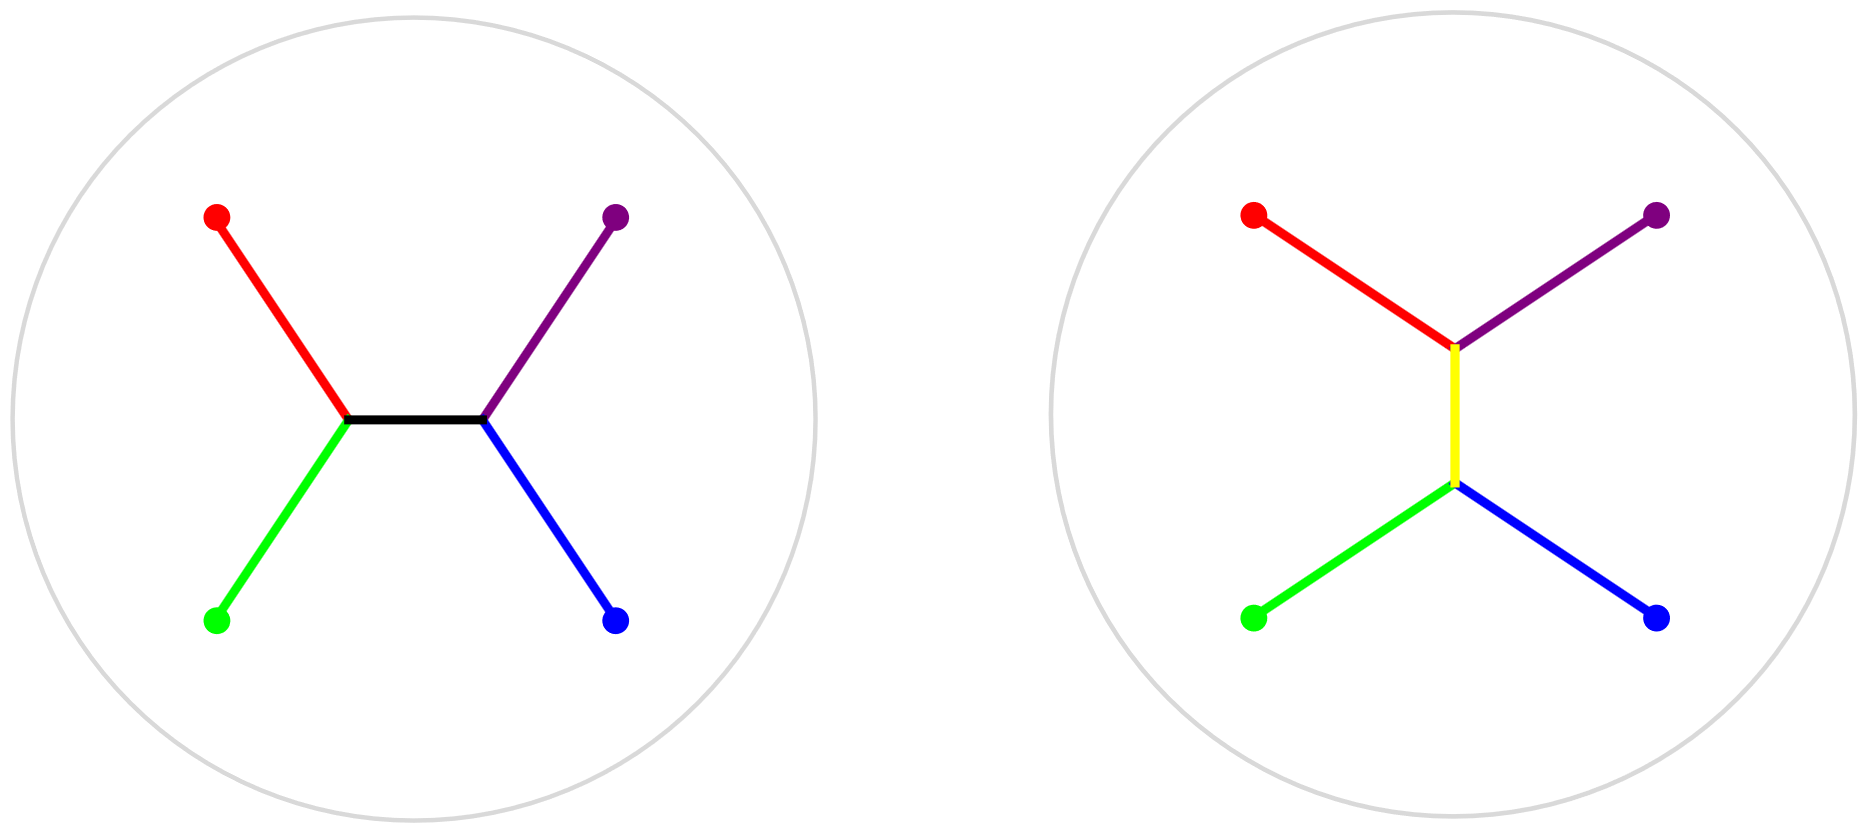
\includegraphics[width=0.85\textwidth]{figures/fig09.png}
  \caption{扭曲扇区算符 $\langle\phi_{g_1}\phi_{g_2}\phi_{g_3}\phi_{g_4}\rangle$ 的球面四点函数，由满足 $g_1g_2g_3g_4=1$ 的拓扑线算符连接。$s$ 道共形块分解涉及结构常数 $C_{g_1,g_2,(g_1g_2)^{-1}}C_{g_3,g_4,g_1g_2}$，而 $t$ 道涉及 $C_{g_2,g_3,(g_2g_3)^{-1}}C_{g_4,g_1,g_2g_3}$（记号只是示意性的，因为我们只用扭曲扇区标记了结构常数中的原初场）。（原文 p.21，图 9）}
  \label{fig:9}
\end{figure}

\begin{figure}[htbp]
  \centering
  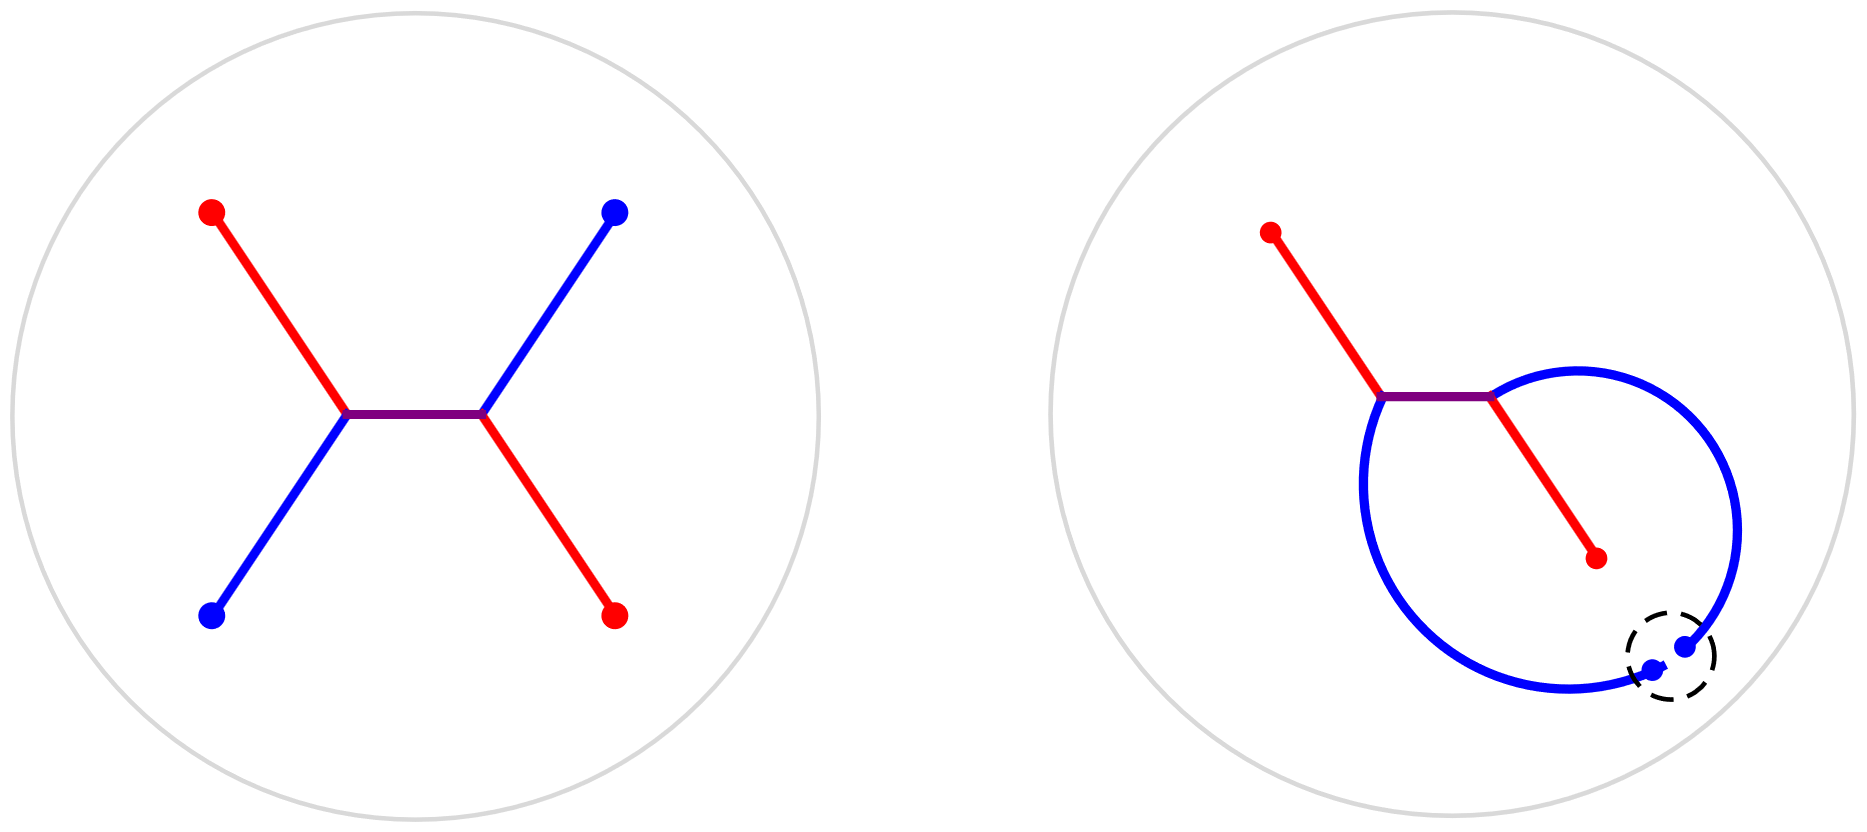
\includegraphics[width=0.85\textwidth]{figures/fig10.png}
  \caption{对于一对对易元素 $g,h$，$u$ 道 OPE 极限下的扭曲场关联函数 $\langle\phi_g\phi_h\phi_{g^{-1}}\phi_{h^{-1}}\rangle$ 决定了最一般的扭曲环面特征标 $Z^g_h$。（原文 p.21，图 10）}
  \label{fig:10}
\end{figure}

作为一个非平凡的实例，考虑基于 Leech 格 $L_{24}$ 的、$c=24$、$\bar c=0$ 的 Narain 格 CFT。$L_{24}$ 是号差为 $(24,0)$ 的偶自对偶格，其特殊性质是不含长度平方等于 $2$ 的格矢量。$L_{24}$ CFT 的环面配分函数为
\begin{equation}
  \label{eq:4-7}
  Z(\tau)=j(\tau)-720,
\end{equation}
其中 $j(\tau)$ 是椭圆 $j$ 不变量
\begin{equation}
  \label{eq:4-8}
  j(\tau)=\frac{E_4(\tau)^3}{\eta(\tau)^{24}}=q^{-1}+744+196884q+21493760q^2+\cdots.
\end{equation}

考虑 $L_{24}$ 的 $\mathbb{Z}_2$ 对称性，其生成元 $g$ 的作用是对所有格元素取反射，即把 24 个手征玻色子全部反射 $X^i_L\to-X^i_L$。相应的环面特征标为
\begin{equation}
  \label{eq:4-9}
  Z^g_1(\tau)=q^{-1}\prod_{n=1}^{\infty}\frac{1}{(1+q^n)^{24}}=\left[\frac{2\eta(\tau)}{\theta_2(\tau)}\right]^{12}.
\end{equation}

% [Tutor Note: (4.9) 的 $\theta$ 函数恒等式可逐步验证：$\theta_2(\tau)=2q^{1/8}\prod_{n\ge1}(1-q^n)(1+q^n)^2$，$\eta(\tau)=q^{1/24}\prod_{n\ge1}(1-q^n)$，故 $\frac{2\eta}{\theta_2}=q^{-1/12}\prod_{n\ge1}(1+q^n)^{-2}$，取 12 次方即得 $q^{-1}\prod_{n\ge1}(1+q^n)^{-24}$。在 $\tau\to-1/\tau$ 下 $\eta\to(-i\tau)^{1/2}\eta$、$\theta_2\to(-i\tau)^{1/2}\theta_4$，比值把 $\theta_2$ 换成 $\theta_4$，于是得到 (4.10)。]

其模 $S$ 变换为
\begin{equation}
  \label{eq:4-10}
  Z^1_g(\tau)=Z^g_1(-1/\tau)=\left[\frac{2\eta(\tau)}{\theta_4(\tau)}\right]^{12}.
\end{equation}
于是轨形 CFT $L_{24}/\mathbb{Z}_2$ 的环面配分函数为
\begin{equation}
  \label{eq:4-11}
  \begin{aligned}
  Z_{L_{24}/\mathbb{Z}_2}(\tau)&=\frac{1}{2}\left[Z^1_1(\tau)+Z^g_1(\tau)+Z^1_g(\tau)+Z^g_g(\tau)\right]\\
  &=\frac{1}{2}j(\tau)-360+2^{11}\bigl(\eta(\tau)\bigr)^{12}\left[\frac{1}{(\theta_2(\tau))^{12}}+\frac{1}{(\theta_4(\tau))^{12}}-\frac{1}{(\theta_3(\tau))^{12}}\right]\\
  &=j(\tau)-744.
  \end{aligned}
\end{equation}

% [Tutor Note: (4.7) 减去 $720$ 而不是 $744$，正是为了抵消 $j$ 的常数项 $744$：$L_{24}$ CFT 的配分函数常数项于是为 $24$，对应 24 个守恒流 $\partial X^i_L$；而 (4.11) 中四项按 $\frac{1}{2}j-360$ 与 $\theta$ 函数组合相加后恰消去常数项，故轨形后无自旋 1 流，这正是下一段所说的“$q^0$ 阶项不出现”。]

特别地，$q^0$ 阶项不出现，说明这个 CFT 中没有守恒的自旋 1 流。$L_{24}/\mathbb{Z}_2$ 轨形实际上具有很大的离散对称群，它同构于最大的散在单群，即 monster 群。这个 CFT 由 Frenkel、Lepowsky 与 Meurman 发现 \cite{r20}，因此也称为 monster CFT。

注意，给定一个 $n$ 阶元素 $g$，我们期望 $Z^1_g(\tau)=Z^g_1(-1/\tau)$ 在 $\tau\to\tau+n$ 下不变。若不成立，则由 $g$ 生成的 $\mathbb{Z}_n$ 所做的轨形就无法自洽地构造。这是离散 't Hooft 反常的一个例子。例如 monster 群有 194 个共轭类，其中 56 个因这类反常不能用来构造轨形。

% [Tutor Note: 这里 $Z^1_g(\tau)=Z^g_1(-1/\tau)$ 是做过 $S$ 变换后的量；若 $g$ 的阶为 $n$，则要求它在 $\tau\to\tau+n$（而不是 $\tau\to\tau+1$）下不变。这正是 $\mathbb{Z}_n$ 轨形自洽的模不变性条件，等价于该对称性没有离散 't Hooft 反常；monster 群的 194 个共轭类中有 56 个不满足，故不能用相应共轭类做轨形。]

\subsection{WZW 与陪集模型}\label{sec:4-3}

一个具有连续对称群 $G$ 的幺正二维 CFT 应当含有一组守恒的 Noether 流 $j^a_\mu$，它们作为局域原初算符出现，$a=1,\cdots,\dim G$。在紧致 CFT 中，这些流必然由权为 $(1,0)$ 的全纯算符 $j^a(z)$ 与权为 $(0,1)$ 的反全纯算符 $\tilde j^a(\bar z)$ 给出。此外，它们的 OPE 必须取流代数的形式；以全纯情形为例，
\begin{equation}
  \label{eq:4-12}
  j^a(z)j^b(0)\sim\frac{\kappa^{ab}}{z^2}+\frac{if^{ab}{}_c\,j^c(0)}{z}.
\end{equation}
这里 $f^{ab}{}_c$ 是 $G$ 的李代数结构常数，$\kappa^{ab}$ 正比于李代数上的一个不变双线性型。幺正性要求 $\kappa^{ab}$ 正定，这意味着 $G$ 半单且紧致。若 $G$ 是单紧致李群，可以写 $\kappa^{ab}=kd^{ab}$，其中 $d^{ab}$ 的逆 $d_{ab}$ 归一化为：对长根 $\psi$ 有 $\psi^2\equiv d_{ab}\psi^a\psi^b=2$。

记 $\hat G_k$ 为单李群 $G$ 的能级 $k$ 流代数。可以定义一个守恒的自旋 2 原初算符，即 Sugawara 能动张量 $T^G$：
\begin{equation}
  \label{eq:4-13}
  T^G(z)=\frac{1}{2(k+h)}\lim_{w\to z}\left[d_{ab}j^a(w)j^a(z)-\frac{k\dim G}{(w-z)^2}\right],
\end{equation}
% [Tutor Note: (4.13) 的被积项写作 $d_{ab}j^a(w)j^a(z)$，第二个流的指标又标成了 $a$。由于 $d_{ab}$ 需要缩并一对指标 $a,b$，这里应为 $d_{ab}j^a(w)j^b(z)$；原文照排，疑为笔误。另外 $2(k+h)$ 中的 $h$ 是下一段才定义的对偶 Coxeter 数，这个整体归一化因子保证 $T^G$ 的 OPE 给出中心荷 (4.14)。]

其中 $h$ 是对偶 Coxeter 数，由关系 $-f^{ac}{}_d f^{bd}{}_c=2h d^{ab}$ 定义。$T^G$ 的归一化使得 $T^G(z)T^G(0)$ 的 OPE 与能动张量的形式相同，其中心荷为
\begin{equation}
  \label{eq:4-14}
  c^G=\frac{k\dim G}{k+h}.
\end{equation}
CFT 能动张量的中心荷 $c$ 大于或等于 $c^G$。若 $c$ 恰等于 $c^G$，则 $T^G$ 也就等于 CFT 的能动张量 $T(z)$。

确实可以构造一个完全自洽的 CFT，其全纯与反全纯能动张量分别为 $T^G(z)$ 与 $\bar T^G(\bar z)$，这就是 Wess–Zumino–Witten（WZW）模型 \cite{r21,r22}。为此需要构造局域算符的谱；这些算符现在不仅可以按 Virasoro 代数的表示来组织，还可以按更大的流代数的表示来组织（因为 Virasoro 生成元可以由流构造出来）。流代数 $\hat G_k$ 的每个不可约表示由一个最低权流代数原初场集合 $\phi_i$ 生成，$\phi_i$ 在 $G$ 的不可约表示 $R$ 中变换，其 OPE 为
\begin{equation}
  \label{eq:4-15}
  j^a(z)\phi_i(0)\sim\frac{t^a_{ij}}{z}\phi_j(0).
\end{equation}
$\hat G_k$ WZW 模型恰好含有一组原初场 $\phi_{i\bar i}(z,\bar z)$，它们与左右流代数群 $G$ 的一对相同表示 $(R,R)$ 相联系；其中 $R$ 遍历 $G$ 的所有不可约表示，其最高权矢量 $\lambda$ 满足 $\langle\lambda,\theta\rangle\le k$，而 $\theta$ 是 $G$ 的最高根矢量。对 $G=SU(2)$，表示 $R$ 由自旋 $j$ 标记，该条件即 $j\le k/2$。

% [Tutor Note: $\langle\lambda,\theta\rangle\le k$ 中的 $\theta$ 取最高根，这一条件把 $\hat G_k$ 的表示限制为可积表示（最高权落在仿射 Weyl 群的 basic alcove 内），从而只留下有限多个幺正表示。对 $SU(2)_k$，自旋 $j$ 的最高权满足 $\langle\lambda,\theta\rangle=2j$，故条件化为 $2j\le k$，即 $j\le k/2$；同一条件用极小模型主场的 Kac 指标写就是 $1\le 2j+1\le k+1$。]

现在给定一个具有连续对称群 $H$、由流代数 $\hat H$ 支配的 CFT，可以尝试规范 $H$ 以得到新的 CFT。把 $\hat G$ WZW 模型的子群 $H\subset G$ 规范化，就得到所谓的 $G/H$ 陪集模型 \cite{r23,r24}。陪集模型完整算符谱的构造相当繁复，这里不详细讨论。注意有一族特殊的陪集模型 $(SU(2)_k\times SU(2)_1)/SU(2)_{k+1}$，它等价于 $A_k$ 极小模型，其中心荷为 $c=1-\frac{6}{(k+2)(k+3)}$。

% [Tutor Note: coset 模型的中心荷按 $c(G_k)-c(H_k)$ 计算；利用 $c(SU(2)_k)=3k/(k+2)$，有 $c=\frac{3k}{k+2}+1-\frac{3(k+1)}{k+3}=1-\frac{6}{(k+2)(k+3)}$，其中 $1=c(SU(2)_1)$ 这一项最容易漏掉。此式与 $A_k$ 极小模型的中心荷公式一致，说明同一 RCFT 可以有多种构造描述。]

\subsection{有理共形场论}\label{sec:4-4}

若一个幺正 CFT 在 Virasoro 代数之外还含有守恒的自旋 $s$ 流，则这些流必然是权为 $(s,0)$ 的全纯流或权为 $(0,s)$ 的反全纯流。先只看全纯算符。全纯算符的 OPE 自行闭合，给出一个扩充 Virasoro 代数的全纯（即手征）顶点算符代数，其一般形式为
\begin{equation}
  \label{eq:4-16}
  \mathcal{O}_a(z)\mathcal{O}_b(0)=\sum_c A_{ab}{}^c z^{-h_a-h_b+h_c}\mathcal{O}_c(0),
\end{equation}
其中 $h_a$ 是非负整数。全纯算符 $\mathcal{O}_a(z)$ 与一个权为 $(h,\tilde h)$ 的一般算符 $\phi$ 的 OPE 只能含有权为 $(h+n,\tilde h)$ 的算符，$n$ 为整数。因此，反全纯权为 $\tilde h$ 的算符集合构成全纯顶点算符代数的一个表示，该表示未必不可约。同样，全纯权为 $h$ 的算符集合构成反全纯顶点代数的一个表示。于是 CFT 的算符谱可以分解为全纯顶点算符代数的表示 $R_i$ 与反全纯顶点代数的表示 $\bar R_{\bar j}$。

$R_i$ 的环面特征标定义为
\begin{equation}
  \label{eq:4-17}
  \chi_i(\tau)=\operatorname{Tr}_{R_i}q^{L_0-\frac{c}{24}},
\end{equation}
类似地有 $\bar R_{\bar i}$ 的特征标 $\bar\chi_{\bar i}(\bar\tau)$。CFT 的环面配分函数可以写成
\begin{equation}
  \label{eq:4-18}
  Z(\tau,\bar\tau)=\sum_{i,\bar i}n_{i\bar i}\,\chi_i(\tau)\bar\chi_{\bar i}(\bar\tau),
\end{equation}
其中 $n_{i\bar i}$ 是非负整数简并度。有理共形场论（RCFT）是指谱中只含有限多个全纯与反全纯顶点算符代数表示的 CFT，即 \eqref{eq:4-18} 是有限和。此时 OPE 的闭合性要求所有权 $(h,\tilde h)$ 都是有理数。

在 $\tau\to\tau+1$ 下，有
\begin{equation}
  \label{eq:4-19}
  \chi_i(\tau+1)=T_{ij}\chi_j(\tau),\qquad T_{ij}=\delta_{ij}e^{2\pi i\left(h_i-\frac{c}{24}\right)}.
\end{equation}
同样有 $\bar\chi_{\bar i}(\bar\tau+1)=\tilde T_{\bar i\bar j}\bar\chi_{\bar j}(\bar\tau)$。环面配分函数的模不变性要求：只有当 $h_i-\tilde h_{\bar j}\in\mathbb{Z}$ 时 $n_{i\bar j}$ 才非零；并且在 $\tau\to-1/\tau$ 下，$\chi_i$ 变为自身的线性组合，$\bar\chi_{\bar i}$ 亦然：
\begin{equation}
  \label{eq:4-20}
  \chi_i(-1/\tau)=S_{ij}\chi_j(\tau),\qquad \bar\chi_{\bar i}(-1/\bar\tau)=\tilde S_{\bar i\bar j}\bar\chi_{\bar j}(\bar\tau),
\end{equation}
使得
\begin{equation}
  \label{eq:4-21}
  n_{i\bar i}S_{ij}\tilde S^*_{\bar i\bar j}=n_{j\bar j}.
\end{equation}

% [Tutor Note: (4.21) 中重复指标 $i,\bar i$ 按 Einstein 约定求和，等式两边的自由指标只剩 $j,\bar j$；它正是 $Z(\tau,\bar\tau)$ 在 $S$ 变换下不变的展开式，$\tilde S^*$ 上的复共轭来自 $\bar\chi$ 的复共轭。用 (4.18) 逐项代入即可得到此式。]

$T$ 与 $S$（以及类似地 $\tilde T$ 与 $\tilde S$）必须构成 $\mathrm{PSL}(2,\mathbb{Z})$ 的有限维表示，即
\begin{equation}
  \label{eq:4-22}
  S^2=(ST)^3=\mathbb{I}.
\end{equation}
这尤其意味着 $(\det S^2)^{-3}(\det(ST)^3)^2=\det T^6=1$，由此可知中心荷 $c$ 也必为有理数。

% [Tutor Note: 这个恒等式值得展开：由 $S^2=\mathbb{I}$ 得 $(\det S)^2=1$，由 $(ST)^3=\mathbb{I}$ 得 $(\det S\det T)^3=1$，于是 $(\det S^2)^{-3}(\det(ST)^3)^2=(\det S)^{-6}(\det S)^6(\det T)^6=\det T^6=1$。又 $\det T=\exp\left(2\pi i\sum_i\left(h_i-\frac{c}{24}\right)\right)$，故 $\sum_i h_i-\frac{nc}{24}\in\frac{1}{6}\mathbb{Z}$；结合 $h_i$ 的有理性即得 $c\in\mathbb{Q}$。]

RCFT 没有完整的分类，尽管所有已明确知道的例子都来自陪集模型或 Narain 格 CFT，及其乘积与轨形，并且位于其精确边缘形变的模空间的特殊点上。最简单的一类 RCFT 是亚纯 CFT（meromorphic CFT），其整个算符谱只由单个全纯顶点算符代数构成，例如前面讨论过的 $L_{24}$ CFT 及其 $\mathbb{Z}_2$ 轨形 monster CFT。即便是亚纯 CFT，也远未得到完整分类。

注意所有 $c>1$ 的 RCFT 都必须含有比 Virasoro 严格更大的全纯顶点算符代数，因为非退化的环面 Virasoro 特征标并不在 $\mathrm{PSL}(2,\mathbb{Z})$ 的有限维表示中变换。换句话说，所有 $c>1$ 的 RCFT 都含有超出 Virasoro 代数的高自旋对称性。

\subsection{非线性 sigma 模型（NLSM）}\label{sec:4-5}

由拉氏量
\begin{equation}
  \label{eq:4-23}
  S=\frac{1}{4\pi}\int d^2\sigma\,\sqrt{g}\,G_{ij}(X)g^{ab}\partial_a X^i\partial_b X^j
\end{equation}
定义的二维非线性 sigma 模型（NLSM）在经典意义上是 Weyl 不变的。若路径积分能以尊重共形对称性的方式正规化，它就会给出一个 CFT，但这远非必然。我们需要研究它的重整化群流：或者分析以 \eqref{eq:4-23} 为基础、配以适当正规化方案由路径积分定义的 1PI 量子有效作用量，或者分析包含所有可能的相关与边缘算符的 Wilson 有效作用量。Wilson 图像在这里相当模糊，因为微扰论中有无穷多个相关算符。其他经典边缘形变具有形式
\begin{equation}
  \label{eq:4-24}
  \frac{1}{4\pi}\int d^2\sigma\,B_{ij}(X)\epsilon^{ab}\partial_a X^i\partial_b X^j+\frac{1}{8\pi}\int d^2\sigma\,\sqrt{g}\,R^{(2)}\Phi(X).
\end{equation}
上式第一项，即 $B$ 场，是宇称奇的。它出现在 WZW 模型的拉氏量描述中：后者相当于群流形 $G$ 上带有非平凡 3-形式通量 $H=dB$ 的 NLSM。第二项涉及二维标量曲率；当 $X$ 为常数时它是拓扑项，在平坦二维时空中消失，其作用是修改能动张量，从而修改场 $X^i$ 的共形变换。这一项例如出现在陪集模型的 NLSM 描述中，最简单的非平凡例子是 $SU(2)/U(1)$ 模型，以及等价于 $SL(2)/U(1)$ 陪集模型的“cigar CFT”。

% [Tutor Note: (4.24) 第二项系数 $\frac{1}{8\pi}$ 与第一项的 $\frac{1}{4\pi}$ 相差因子 2，来源是 $\sqrt{g}R^{(2)}$ 的标准归一化；若改用 $\frac{1}{4\pi\alpha'}$ 的拉氏量约定，两式的相对系数会随之改变。当 $X$ 为常数时第二项化为 $\chi(\Sigma)\Phi$ 型的拓扑项（Gauss–Bonnet 定理），在环面（$\chi=0$）上确实消失；注意 $\chi=0$ 的是环面，而非任意平坦时空。]

至少在无 $B$ 场时，可以用维数正规化（形式上在 $d=2-\epsilon$ 维工作）直接正规化路径积分，并微扰地计算 1PI 有效作用量，或更直接地计算能动张量的迹：
\begin{equation}
  \label{eq:4-25}
  T^a{}_a=-\frac{\epsilon}{2}G_{ij}(X)\partial^a X^i\partial_a X^j+\frac{\epsilon}{4}R^{(2)}\Phi(X)-\frac{1}{2}\nabla_X^2\Phi(X).
\end{equation}
要把它变成量子理论中有意义的算符方程，需要把右边用重整化算符改写，然后取 $\epsilon\to0$ 极限。最终得到如下形式的算符方程：
\begin{equation}
  \label{eq:4-26}
  T^a{}_a=\frac{1}{2}\left[\beta^G_{ij}(X)\partial^a X^i\partial_a X^j\right]_r-\frac{1}{4}R^{(2)}\left[\beta^\Phi(X)\right]_r,
\end{equation}
其中 $[\cdots]_r$ 表示某种算符正规化，$\beta^G_{ij}$ 与 $\beta^\Phi$ 到前两个非平凡微扰阶为 \cite{r25}
\begin{equation}
  \label{eq:4-27}
  \begin{aligned}
  \beta^G_{ij}&=R_{ij}+\frac{1}{2}R_i{}^{k\ell m}R_{jk\ell m}+2\nabla_i\nabla_j\Phi+\cdots,\\
  \beta^\Phi&=-\nabla^2\Phi+(\nabla\Phi)^2+\frac{1}{4}R^{ijk\ell}R_{ijk\ell}+\cdots.
  \end{aligned}
\end{equation}

% [Tutor Note: (4.27) 中 $\frac{1}{2}R_i{}^{k\ell m}R_{jk\ell m}$ 是二圈引力 beta 函数的标志项，$\beta^\Phi$ 的一圈部分是 $-\nabla^2\Phi+(\nabla\Phi)^2$，二圈部分则是 $\frac{1}{4}R^{ijk\ell}R_{ijk\ell}$；若在 $\beta^G_{ij}$ 中把 $R_{ij}$ 也一并按“一圈+二圈”分组，则它分别对应量纲 2 与量纲 4 的算符。注意 $R_i{}^{k\ell m}$ 的第一个指标在上、其余在下，与 $R_{jk\ell m}$ 缩并后得到对称张量；指标位置摆错会差一个符号。]

共形不变性等价于条件 $\beta^G_{ij}=\beta^\Phi=0$。事实上，后者等价于基于有效作用量 $S_{\rm eff}[G_{ij}(X),\Phi(X)]$ 的靶空间运动方程。这些方程可以在靶空间局部求解，但解的整体存在性——尤其当靶空间紧致时——远非显然。

% ch04b.tex —— Xi Yin, Aspects of Two-Dimensional Conformal Field Theories（PoS TASI2017）中译
% 覆盖 PDF 第 27–33 页（原书 p.26–32）：4.5 节续文、4.6 超共形对称性、4.7 Calabi–Yau 模型、
% 4.8 精确边缘形变、4.9 RG 流。另补译 PDF 第 34 页顶部至第 4 节结束的文字（含 (4.46)），使第 4 节完整收束。
% 本区间无图。公式编号沿用原文 (4.28)–(4.46)，文献 [N] 一律对应参考文献键 rN。译者：tr04b。

例如，领头阶条件 $R_{ij}=0$ 等价于 NLSM 单圈 beta 函数的消失，它要求靶空间 Ricci 平坦。这给靶空间加上了很不平凡的拓扑限制。一类允许 Ricci 平坦度规的偶数维紧致流形是 Calabi--Yau 流形。可以问：给定 Ricci 平坦度规为 $G_{ij}(X)$ 的 Calabi--Yau 流形 $M$，能否开启膨胀子剖面 $\Phi(X)$ 并形变度规，使 \eqref{eq:4-27} 在全阶都被解出？我不知道这个问题的答案；不过，这个问题的超共形版本答案是肯定的，下一小节就来讨论。

% [Tutor Note: 这里提到的 (4.27) 是上一小节给出的含膨胀子的 NLSM $\beta$ 函数方程（已含二圈项）；其领头阶只留下 $R_{ij}+2\nabla_i\nabla_j\Phi$，故只保留度规项时给出 $R_{ij}=0$。作者强调“全阶”可解，是因为 $\alpha'$ 修正会引入高阶曲率项。]

\subsection{超共形对称性}

带超对称的 CFT 妙处很多：其中之一是这类理论大量存在，而由于各种超对称非重整化性质，证明它们存在往往很容易。Poincaré 超对称与共形对称不对易，两者合起来生成超共形对称群。超共形代数（SCA）由自旋 $\frac32$ 流的个数 $\mathcal{N}$ 刻画（但不唯一）。已知有 CFT 容许 $\mathcal{N}=1$、$2$、$4$ 的全纯与反全纯 SCA。

$\mathcal{N}=4$ SCA 分两类，性质很不一样：小的 $\mathcal{N}=4$ SCA 只含一个 $SU(2)$“R 对称性”流代数；大的 $\mathcal{N}=4$ SCA 含 $SU(2)\times SU(2)\times U(1)$ 流代数。

SCA 是对玻色 Virasoro 代数的扩充，因此超共形场论（SCFT）可以看作带额外高自旋对称性的普通玻色 CFT，但有一个重要的微妙之处：SCA 含半整数自旋流，这似乎破坏柱面上的动量量子化，也破坏模不变性。要让理论自洽，有两条路：要么稍微放宽模不变性的通常概念，允许谱中出现半整数自旋算符；要么坚持整数自旋条件，把半整数自旋算符从谱中投影掉。后者称为 Gliozzi--Scherk--Olive（GSO）投影 \cite{r26}，做法如下。半整数自旋算符是反对易场，具有奇费米子数 $F$；$F$ 是模 $2$ 意义下的整数。投影到整数自旋算符，等于投影到 $(-)^F$ 不变的态。要与模不变性相容，还必须纳入关于 $(-)^F$ 的扭曲扇区态。在 GSO 投影后的理论中，半整数自旋的超共形流严格说并不在谱内，但仍可用它们按 SCA 的表示来组织谱。

下面讨论 SCA 的几个例子（远非穷尽）以及实现这些对称性的 CFT。先从 $\mathcal{N}=1$ SCA 开始：除中心荷为 $c$ 的能动张量 $T(z)$ 外，它只含一个自旋 $\frac32$ 的反对易场 $G(z)$，且 $G(z)$ 是 Virasoro 原初场。唯一新的独立 OPE 关系是
\begin{equation}
  \label{eq:4-28}
  G(z)G(0)\sim\frac{2c}{3z^3}+\frac{2}{z}T(0).
\end{equation}
作用在原点处的态上时，用 Laurent 级数
\begin{equation}
  \label{eq:4-29}
  G(z)=\sum_{r\in\mathbb{Z}+\nu}\frac{G_r}{z^{r+\frac32}}
\end{equation}
更方便。

% [Tutor Note: $\nu=\frac12$ 时 $r\in\mathbb{Z}+\frac12$，对应 NS 扇区；$\nu=0$ 时 $r\in\mathbb{Z}$，对应 R 扇区。作者用同一个 $\nu$ 统一写出两种展开，这是核对 (4.36)–(4.38) 中 $q$ 的幂次与模指标时最容易出错的地方：NS 扇区态按半整数模指标计数，R 扇区态按整数模指标计数。]

其中在无支割线时 $\nu=\frac12$。此时称原点处的算符处于 Neveu--Schwarz（NS）扇区。特别地，单位算符属于 NS 扇区。GSO 投影要求存在扭曲扇区算符，并在其上附着一条与 $(-)^F$ 相伴的拓扑线算符。这条拓扑线算符造成一条支割线，结果 $G(z)$ 的 Laurent 级数 \eqref{eq:4-29} 中 $\nu=0$。这类扭曲扇区算符称为 Ramond（R）扇区算符。

$\mathcal{N}=(1,1)$ SCFT 的一些基本例子，是中心荷 $c=\frac32-\frac{12}{(k+2)(k+4)}$（$k=1,2,\cdots$）的 $\mathcal{N}=1$ 极小模型。有趣的是，GSO 投影后的 $\mathcal{N}=1$ 极小模型也可实现为玻色陪集模型 $(SU(2)_k\times SU(2)_2)/SU(2)_{k+2}$。另一些例子包括自由 $c=\frac32$ 理论，它由一个紧致玻色子和一对互为手征、反手征的自由费米子 $\psi,\tilde\psi$ 组成；还有 $\mathcal{N}=1$ Liouville CFT：在拉氏量层面，它可以看作线性膨胀子 CFT 加上自由费米子 $\psi,\tilde\psi$，并在领头阶受到形式为 $\psi\tilde\psi e^{\beta\phi}$ 的边缘算符形变。

接着考虑 $\mathcal{N}=2$ SCA。它有一对自旋 $\frac32$ 的反对易场 $G^\pm(z)$ 和一个 $U(1)$ R 流 $J(z)$。可把 $J(z)$ 归一化，使其 OPE 取形式
\begin{equation}
  \label{eq:4-30}
  J(z)J(0)\sim\frac{c}{3z^2},
\end{equation}
此时 $G^\pm$ 相对 $J(z)$ 带电荷 $\pm1$。$G^+G^+$ 与 $G^-G^-$ 的 OPE 非奇异。唯一新的非平凡 OPE 关系是
\begin{equation}
  \label{eq:4-31}
  G^+(z)G^-(0)\sim\frac{2c}{3z^3}+\frac{2}{z^2}J(0)+\frac{2}{z}T(0)+\frac{1}{z}\partial J(0).
\end{equation}

% [Tutor Note: (4.31) 末项系数极易按记忆写成 $2$。作者采用 $\{G^+_r,G^-_s\}=2L_{r+s}+(r-s)J_{r+s}+\frac{c}{3}(r^2-\frac14)\delta_{r+s,0}$ 与 $J(z)J(0)\sim\frac{c}{3z^2}$ 的归一化：用 $[J_2,\cdot]$ 作用于 (4.31) 两边（$[J_2,G^\pm(z)]=\pm z^2G^\pm(z)$，$[J_2,\partial J(0)]=\frac{2c}{3}$），即定出该系数为 $1$。]

用 Laurent 模式 $G^\pm_r,L_n,J_n$ 表示，$\mathcal{N}=2$ SCA 有一个外自同构，称为谱流：
\begin{equation}
  \label{eq:4-32}
  G^\pm_r\to G^\pm_{r\pm\eta},\qquad J_n\to J_n+\eta\frac{c}{3}\delta_{n,0},\qquad L_n\to L_n+\eta J_n+\eta^2\frac{c}{6}\delta_{n,0},
\end{equation}
其中 $\eta\in\mathbb{Z}$。也可以把谱流延拓到半整数 $\eta$，它连接 NS 与 R 扇区。不过，谱流不必是 SCFT 的对称性。

某些“好”的 $\mathcal{N}=2$ SCFT 确实具有谱流对称性。一个例子是 Calabi--Yau 靶空间上的 $(2,2)$ NLSM。此时可按 $\mathcal{N}=2$ SCA 加上谱流对称性（$\eta$ 取整数或半整数）生成的更大对称性来组织算符谱。这称为“扩展 $\mathcal{N}=2$ SCA”\cite{r27,r28}。

% [Tutor Note: 谱流 (4.32) 只是 $\mathcal{N}=2$ SCA 的外自同构，一般不保持谱；在 Calabi--Yau 上的 $(2,2)$ NLSM 里它成为真正的对称性，原因是靶空间的复结构给出额外的整体 $U(1)$，使整数（乃至半整数）$\eta$ 的谱流把谱映回自身。正因如此，下文的 Calabi--Yau 模型才能用扩展 $\mathcal{N}=2$ SCA 的表示论描述 BPS 谱，而不必处理一般 $\mathcal{N}=2$ SCA 的种种缩短表示。]

$\mathcal{N}=2$ SCFT 的其他例子包括 $\mathcal{N}=2$ 极小模型，$c=\frac{3k}{k+2}$，$k=1,2,\cdots$。注意它们的中心荷与 $SU(2)_k$ WZW 模型相同，但并不是同一个 CFT（特别是算符谱不同）。另一个非平凡例子是 $\mathcal{N}=2$ Liouville CFT \cite{r29}：在拉氏量层面，它可以看作紧致玻色子加线性膨胀子再加一对费米子，并在领头阶受到形式为 $\psi_+\tilde\psi_+e^{-\beta\varphi}+\psi_-\tilde\psi_-e^{-\beta\bar\varphi}$ 的边缘算符形变。

最后讨论小的 $\mathcal{N}=4$ SCA。它有四个自旋 $\frac32$ 的流 $G^{\alpha A}(z)$，其中 $\alpha$ 是关于 $SU(2)_k$ R 流 $J_i(z)$ 的二重态指标，$c=6k$；$A$ 是一个额外指标，在外自同构 $SU(2)_{\mathrm{out}}$ 下变换，后者不属于超共形对称性，一般也不是 SCFT 的对称性。注意 $SU(2)$ 能级 $k$ 是整数，故 $c$ 必须是 $6$ 的整数倍。唯一新的非平凡 OPE 关系是
\begin{equation}
  \label{eq:4-33}
  G^{\alpha A}(z)G^{\beta B}(0)\sim\varepsilon^{AB}\Big[\frac{2c}{3z^3}\varepsilon^{\alpha\beta}
  +\sigma_i^{\alpha\beta}\frac{2}{z^2}J_i(0)+\varepsilon^{\alpha\beta}\frac{2}{z}T(0)
  +\sigma_i^{\alpha\beta}\frac{1}{z}\partial J_i(0)\Big].
\end{equation}

% [Tutor Note: (4.33) 中 $\sigma_i^{\alpha\beta}$（$i=1,2,3$）是 $SU(2)$ 的 Pauli 矩阵，$\varepsilon^{\alpha\beta}$、$\varepsilon^{AB}$ 是反对称张量；方括号内四项分别是中心项、R 流、能动张量与 R 流的导数，指标缩并方式决定整体符号。小 $\mathcal{N}=4$ 的 $c=6k$ 与式中的 $2c/3=4k$ 一致，可用它快速检验系数。]

$\mathcal{N}=4$ SCA 也容许谱流映射
\begin{equation}
  \label{eq:4-34}
  G^{\pm A}_r\to G^{\pm A}_{r\pm\eta},\qquad J^3_n\to J^3_n+\eta k\delta_{n,0},\qquad
  J^\pm_n\to J^\pm_{n\pm2\eta},\qquad L_n\to L_n+2\eta J^3_n+\eta^2k\delta_{n,0},
\end{equation}
其中 $\eta$ 为整数（半整数 $\eta$ 会联系 NS 与 R 扇区）。这里相当不平凡的是，谱流本身是 $\mathcal{N}=4$ SCA 的一部分；换句话说，与 $\mathcal{N}=2$ SCA 不同，小 $\mathcal{N}=4$ SCA 自动是“扩展”的。这可通过研究 $\mathcal{N}=4$ SCA 的真空特征标并看出它在谱流下不变来证明。

% [Tutor Note: 对比 (4.32) 与 (4.34)：$\mathcal{N}=2$ 时 $J_n$ 的平移量是 $\eta c/3$，$\mathcal{N}=4$ 时 $J^3_n$ 的平移量是 $\eta k=\eta c/6$，而 $L_n$ 的二次项分别是 $\eta^2c/6$ 与 $\eta^2k=\eta^2c/6$，两处一致。注意 $J^\pm_n$ 的指标平移是 $2\eta$、而 (4.32) 中 $G^\pm_r$ 的平移是 $\pm\eta$：两式对谱流参数 $\eta$ 的归一化约定不同，合读时不要按同一 $\eta$ 数值代换。]

小 $\mathcal{N}=4$ SCA 的表示论相对简单：幺正表示由权 $h$ 与 $SU(2)_R$ 自旋 $\ell$ 标记，$\ell$ 取有限范围 \cite{r30}。在 NS 扇区，非 BPS 原初态满足 $h>\ell$，$\ell=0,\frac12,\cdots,\frac{k-1}{2}$；BPS 原初态满足 $h=\ell$，$\ell=0,\frac12,\cdots,\frac{k}{2}$。

容许小 $\mathcal{N}=4$ SCA 的 SCFT 的一类非平凡例子，是 hyperKähler 流形上的超对称 NLSM。另有一族 $\mathcal{N}=4$ Liouville 理论 \cite{r31}，中心荷 $c=6k$，可由线性膨胀子、四个自由费米子与 $SU(2)_{k-1}$ WZW 模型组成的 CFT 经边缘形变构造。

\subsection{Calabi--Yau 模型}

Calabi--Yau $d$ 重流形上的超对称 NLSM 配上一族合适的度规和可能的 $B$ 场（它们解出经 $\alpha'$ 修正的 Ricci 平坦条件），定义了一族 $c=3d$、具有扩展 $\mathcal{N}=2$ SCA 的 $\mathcal{N}=(2,2)$ SCFT。特别地，全纯 NS 扇区上的 $\eta=1$ 谱流把单位算符（NS 扇区真空态）映成权 $h=\frac d2$、$U(1)_R$ 荷为 $d$ 的超共形原初算符 $\mathcal{O}_\Omega$。并且 $\mathcal{O}_\Omega$ 被 $G^+_{-\frac12}$ 湮灭，是一个手征原初算符。它在 NLSM 描述里有自然的解释：存在全纯 $d$-形式 $\Omega=\frac{1}{d!}\Omega_{i_1\cdots i_d}dz^{i_1}\wedge\cdots\wedge dz^{i_d}$，由此可构造算符
\begin{equation}
  \label{eq:4-35}
  \mathcal{O}_\Omega\sim\Omega_{i_1\cdots i_d}\psi^{i_1}\cdots\psi^{i_d}.
\end{equation}
在相互作用 NLSM 中，右端先验地需要正规化；但实际上由于 $\Omega$ 的全纯性，这样的算符不会被重整化（注意 $\bar z^{\bar i}$ 与 $\bar\psi^{\bar i}$ 都不出现）。

% [Tutor Note: $\mathcal{O}_\Omega$ 是 $(c,c)$ 环中的手征原初算符：它是 $(d,0)$ 形式与手征费米子的缩并，全纯性使它不受 $\bar z$、$\bar\psi$ 方向的短距离奇异性影响，因而不被重整化。这类算符在拓扑 twist 后成为拓扑弦的可观测量，也是下文计数 BPS 态的出发点。]

到目前为止，我们对作为 SCFT 的 Calabi--Yau 模型的认识，大体限于精确边缘形变的模空间、BPS 算符谱，以及由共形自举得到的关于非 BPS 算符谱的一些粗糙限制。例外是模空间中的一些特殊点（称为 Gepner 点），那里的 SCFT 恰好是有理的，并可描述为极小模型乘积的轨形。

下面简述算符谱。一般 $\mathcal{N}=2$ SCA 的表示论相当精细 \cite{r32,r33}，包含多种不同的缩短表示；扩展 $\mathcal{N}=2$ SCA 的表示论则相对简单 \cite{r27,r28}。在全纯与反全纯两侧各自独立地，存在非 BPS（有质量）表示与 BPS（无质量）表示。非 BPS 表示含一个超共形原初态，其 R 荷 $Q$ 取整数值，范围是 $Q=0,\pm1,\pm2,\cdots,\pm(\lfloor d/2\rfloor-1)$，$d$ 为奇数时还有 $\frac{d-1}{2}$；它满足 BPS 界 $h>\frac{|Q|}{2}$。非 BPS 表示的全部权与荷内容由下面的 NS 特征标概括：
\begin{equation}
  \label{eq:4-36}
  \begin{aligned}
    ch^{NS}_{h,Q}(q,y)&\equiv\mathrm{Tr}_{\text{non-BPS}}\,q^{L_0-\frac{c}{24}}y^{J_0}\\
    &=q^{h-\frac{c}{24}}\sum_{m=-\infty}^{\infty}q^{\frac{d-1}{2}m^2+mQ}y^{(d-1)m+Q}
    \prod_{n=1}^{\infty}\frac{(1+yq^{n-\frac12})(1+y^{-1}q^{n-\frac12})}{(1-q^n)^2}
  \end{aligned}
\end{equation}

另一方面，BPS 表示含一个手征或反手征原初态，其 R 荷 $Q$ 取整数值，范围是 $Q=0,\pm1,\pm2,\cdots,\pm\big\lfloor\frac{d-1}{2}\big\rfloor$，$d$ 为偶数时还有 $\frac d2$；它饱和 BPS 界 $h=\frac{|Q|}{2}$。相应的 NS 特征标 $\chi^{NS}_Q(q,y)\equiv\mathrm{Tr}_{\text{BPS}}\,q^{L_0-\frac c{24}}y^{J_0}$ 由下式给出：
\begin{equation}
  \label{eq:4-37}
  \begin{aligned}
    \chi^{NS}_Q(q,y)&=q^{\frac Q2-\frac c{24}}\sum_{m\in\mathbb{Z}}\frac{q^{\frac{d-1}{2}m^2+mQ}y^{(d-1)m+Q}}{1+yq^{m+\frac12}}
      \prod_{n=1}^{\infty}\frac{(1+yq^{n-\frac12})(1+y^{-1}q^{n-\frac12})}{(1-q^n)^2},\quad Q>0,\\
    \chi^{NS}_Q(q,y)&=\chi^{NS}_{-Q}(q,y^{-1}),\quad Q<0,\\
    \chi^{NS}_0(q,y)&=q^{-\frac c{24}}\sum_{m\in\mathbb{Z}}\frac{(q^{-\frac12}-q^{\frac12})q^{\frac{d-1}{2}m^2+m}y^{(d-1)m+1}}{(1+yq^{m-\frac12})(1+yq^{m+\frac12})}
      \prod_{n=1}^{\infty}\frac{(1+yq^{n-\frac12})(1+y^{-1}q^{n-\frac12})}{(1-q^n)^2}.
  \end{aligned}
\end{equation}

% [Tutor Note: (4.36) 与 (4.37) 的差别只在分母上的 $(1+yq^{m+\frac12})$ 型因子：非 BPS 表示不缩短，直接对谱流轨道求和；BPS 表示被 $h=\frac{|Q|}{2}$ 缩短，$Q>0$ 时留下 $1+yq^{m+\frac12}$ 的零点，$Q<0$ 由 $\chi^{NS}_Q(q,y)=\chi^{NS}_{-Q}(q,y^{-1})$ 镜像给出，$Q=0$ 则靠 $(q^{-\frac12}-q^{\frac12})$ 抵消分母的零点。核对 (4.36)–(4.37) 时最容易丢掉这些因子。]

同时在两侧都属于 BPS 表示的算符，笼统称为 $\frac12$-BPS；一侧 BPS、另一侧非 BPS 的算符，则称为 $\frac14$-BPS。

有一个超对称指数对约束 $\frac12$-BPS 与 $\frac14$-BPS 算符的谱非常有用，即椭圆亏格 \cite{r34}。定义这个指数必须在基态保持超对称的 Ramond 扇区里做。R 扇区特征标与 NS 扇区特征标由 $\eta=\frac12$ 的谱流相联系，代价是原初权与 R 荷的平移：
\begin{equation}
  \label{eq:4-38}
  ch^{R}_{h,Q}(q,y)=ch^{NS}_{h+\frac c{24}-\frac Q2,\frac c6-Q}\big(q,q^{\frac12}y\big),\qquad
  \chi^{R}_Q(q,y)=\chi^{NS}_{\frac c6-Q}\big(q,q^{\frac12}y\big).
\end{equation}

椭圆亏格定义为 (R,R) 扇区中的特征标，形如
\begin{equation}
  \label{eq:4-39}
  \chi(\tau,z)=\mathrm{Tr}_{RR}\,q^{L_0-\frac c{24}}y^{J_0}\bar q^{\bar L_0-\frac c{24}}e^{\pi i\bar J_0},
\end{equation}
其中 $q=e^{2\pi i\tau}$，$y=e^{2\pi iz}$。注意 $\bar\tau$ 依赖会消失，原因是反全纯 R 荷 $\bar J_0$ 为偶与为奇的激发态之间发生相消。由于（整数 $\eta$ 的）谱流对称性，$\chi$ 在 $z\to z+1$ 与 $z\to z+\tau$ 下不变。此外，$\chi$ 具有 $PSL(2,\mathbb{Z})$ 变换性质
\begin{equation}
  \label{eq:4-40}
  \chi(\tau+1,z)=\chi(\tau,z),\qquad
  \chi(-1/\tau,z/\tau)=e^{2\pi i\frac d2\frac{z^2}{\tau}}\chi(\tau,z).
\end{equation}

% [Tutor Note: (4.39) 中 $e^{\pi i\bar J_0}$ 与 $\bar q^{\bar L_0-\frac c{24}}$ 合起来实现 $(-)^{\bar J_0}$ 加权，反全纯 R 荷奇偶的态两两相消，这就是 $\bar\tau$ 依赖消失的原因；能存活下来的正是被 $\bar G^-_{-\frac12}$、$\bar G^+_{-\frac12}$ 湮灭的 BPS 态。指标 $d/2$ 等于 $\eta=\frac12$ 谱流对 $J_0$ 的平移量 $c/6$，这也是 (4.40) 中 $e^{2\pi i\frac d2\frac{z^2}{\tau}}$ 因子的来源。]

也就是说，$\chi(\tau,z)$ 是权 $0$、指标 $\frac d2$ 的弱 Jacobi 形式。整数指标的弱 Jacobi 形式空间由四个基本 Jacobi 形式 $E_4,E_6,\phi_{0,1},\phi_{-2,1}$ 的多项式张成，其中 $E_4,E_6$ 是 Eisenstein 级数，$\phi_{0,1},\phi_{-2,1}$ 是两个指标 $1$ 的弱 Jacobi 形式。对半整数指标，还可额外使用另外两个基本弱 Jacobi 形式 $\phi_{0,\frac32}$ 与 $\phi_{-1,\frac12}$。

$d=2$ 时（例子是靶空间为 K3 的 SCFT），椭圆亏格必须正比于 $\phi_{0,1}$。把 Witten 指数与 K3 的 Euler 示性数匹配，可得 \cite{r35}
\begin{equation}
  \label{eq:4-41}
  \chi_{\mathrm{K3}}(\tau,z)=2\phi_{0,1}(\tau,z)=2y+20+2y^{-1}+(20y^2-128y+216-128y^{-1}+20y^{-2})q+\cdots.
\end{equation}
在假定小 $\mathcal{N}=4$ SCA 之外没有额外守恒高自旋流的前提下，这可以用来确定 K3 CFT 中所有 $\frac12$-BPS 与 $\frac14$-BPS 态的简并度。

% [Tutor Note: 系数 $2$ 由 Witten 指数定出：$\phi_{0,1}$ 在 $y=1$ 处给 $12$，故 $2\phi_{0,1}$ 给 $24=\chi(\mathrm{K3})$。$q^0$ 层的 $2y+20+2y^{-1}$ 就是 K3 上 $\frac12$-BPS 态的计数；能如此干净地逐层读出简并度，前提正是小 $\mathcal{N}=4$ 之外没有额外高自旋流。]

$d=3$ 时（含 Calabi--Yau 三重流形模型），椭圆亏格必须正比于 $\phi_{0,\frac32}$。把 Witten 指数与 Euler 示性数匹配，得到
\begin{equation}
  \label{eq:4-42}
  \chi_{\mathrm{CY}_3}(\tau,z)=(h^{1,1}-h^{2,1})\phi_{0,\frac32}(\tau,z).
\end{equation}
于是可以把 $\phi_{0,\frac32}(\tau,z)$ 按 RR 扇区的扩展 $\mathcal{N}=2$ 特征标分解。结果很简单：$\phi_{0,\frac32}=\chi^R_1-\chi^R_{-1}$。这个结果对 BPS 谱有有趣的推论：虽然有（扩展 $\mathcal{N}=2$）$\frac12$-BPS 多重态对应 SCFT 的形变模，但 $\frac14$-BPS 多重态要么含有额外守恒的高自旋流（预期在共形流形的一般点上不存在），要么必须两两配对，从而可能在边缘形变下被提升为非 BPS 多重态。

% [Tutor Note: 分解式 $\phi_{0,\frac32}=\chi^R_1-\chi^R_{-1}$ 中，$\chi^R_1$ 与 $\chi^R_{-1}$ 分别是 $Q=\pm1$ 的 BPS 表示，正负号来自 R 扇区中手征与反手征表示的符号。系数只有 $\pm1$，故 $\frac14$-BPS 态无法单独出现，只能配对或伴生高自旋流，这正是这段推理的关键。]

\subsection{精确边缘形变}

当 CFT 容许一个权 $h=\tilde h=1$ 的边缘原初算符 $\mathcal{O}$ 时，可以在关联函数中插入 $\exp[-\lambda\int d^2z\,\mathcal{O}(z,\bar z)]$ 来形变理论。对有拉氏量描述的理论，这相当于把拉氏量密度用算符 $\mathcal{O}(z,\bar z)$ 形变。共形不变性在形变参数 $\lambda$ 的一阶保持；更高阶一般不保持，因为重合算符的正规化会破坏共形对称性。例如，若 $\mathcal{O}(z,\bar z)\mathcal{O}(0)$ 的 OPE 含另一个边缘原初算符，就会在 $\lambda^2$ 阶生成非平凡的 beta 函数。

% [Tutor Note: “正规化”指重合点 $z\to0$ 处 $\mathcal{O}(z,\bar z)\mathcal{O}(0)$ 的短距离奇异性必须截断；若 OPE 中出现另一边缘算符 $\mathcal{O}'$，重整化会生成正比于 $\lambda^2\int\mathcal{O}'$ 的反项，beta 函数因此非零。注意作者把形变写成 $\exp[-\lambda\int]$，与部分文献用 $g\int$ 的符号约定相反，比较公式时留意。]

理解更高阶共形不变性障碍的一个有用办法，是把该 CFT 看作紧致化玻色弦世界面理论的一部分，连同自由玻色子 $X^\mu$ 与 $b,c$ 鬼场。一个边缘原初算符给出 Minkowski 时空（由 $X^\mu$ 参数化）中无质量标量场的顶点算符 $\mathcal{V}_i=\mathcal{O}e^{ik_i\cdot X}$。共形不变性的第 $n$ 阶障碍，由 $n$ 点弦树图散射振幅在 $k_i\to0$ 同时极限下的值刻画：
\begin{equation}
  \label{eq:4-43}
  \Big\langle\Big[\prod_{i=1}^{n-3}\int d^2z_i\,\mathcal{V}_i(z_i,\bar z_i)\Big]
  \mathcal{V}_{n-2}(0)\mathcal{V}_{n-1}(1)\mathcal{V}'_n(\infty)\Big\rangle,
\end{equation}
其中 $z_i$ 积分可通过对 $k_i$ 的解析延拓正规化。

% [Tutor Note: (4.43) 是固定 $SL(2,\mathbb{C})$ 后剩下的 $n-3$ 个重积分；$\mathcal{V}'_n(\infty)$ 表示在无穷远处按共形权插入顶点算符。所谓“零动量极限的障碍”是指：若该振幅在 $k_i\to0$ 时不消失，有效作用量就会生成相应局域反项，破坏共形不变性。$d^2z_i$ 积分在 $k_i$ 非零时发散，作者用 $k_i$ 的解析延拓来定义它，这是 Polchinski 共形微扰论的标准做法。]

精确边缘形变是导致一族连续 CFT 的边缘形变，由形变参数 $\lambda$ 参数化。这要求 \eqref{eq:4-43} 的零动量极限对所有 $n$ 都消失。这个形变空间上有自然的度规概念，由边缘算符的两点函数给出，称为 Zamolodchikov 度规 \cite{r36}。因此，精确边缘形变的这个模空间是 Riemann 流形，有时称为共形流形。基本例子是基于 Narain 格 $\Gamma_{n_L,n_R}$ 的自由玻色子 CFT，它有 $n_Ln_R$ 维共形流形，同构于 $\mathrm{Aut}(\Gamma_{n_L,n_R})\backslash O(n_L,n_R)/(O(n_L)\times O(n_R))$。更一般地，只要 CFT 有一组 $U(1)^{n_L}$ 全纯流 $j^a_z$ 与 $U(1)^{n_R}$ 反全纯流 $\bar j^b_{\bar z}$，则形变 $j^a_z\bar j^b_{\bar z}$ 都精确边缘。

% [Tutor Note: Narain 情形的模空间维数是 $n_Ln_R$，不是 $n_L^2+n_R^2$：商空间里左乘 $\mathrm{Aut}(\Gamma_{n_L,n_R})$ 是格自同构，右除的 $O(n_L)\times O(n_R)$ 分别是左右手征基的转动。$j^a_z\bar j^b_{\bar z}$ 之所以精确边缘，是因为流守恒 $\bar\partial j=0$ 使形变的 OPE 里不会出现会生成 beta 函数的边缘算符。]

现在讨论 $(2,2)$ SCFT 的边缘形变，它们一阶保持全部超共形对称性。这类形变基于权 $(\frac12,\frac12)$ 的（手征，手征）或（手征，反手征）算符，通过形如
\begin{equation}
  \label{eq:4-44}
  \mathcal{O}=G^-_{-\frac12}\bar G^-_{-\frac12}\phi^{+,+}+G^+_{-\frac12}\bar G^+_{-\frac12}\phi^{-,-}
  \quad\text{or}\quad
  G^-_{-\frac12}\bar G^+_{-\frac12}\phi^{+,-}+G^+_{-\frac12}\bar G^-_{-\frac12}\phi^{-,+}
\end{equation}
的后代实现，其中 $\phi^{+,+}$ 表示全纯与反全纯 $U(1)_R$ 荷为 $(1,1)$ 的（手征，手征）原初场，$\phi^{+-}$ 表示 R 荷为 $(1,-1)$ 的（手征，反手征）原初场。要看出这保持超共形对称性，需证明对任意全纯函数 $v(z)$，超共形流 $v(z)G^+(z)$ 可移过 $\mathcal{O}(w,\bar w)$ 而只差一个全导数。在（手征，手征）情形验证如下：
\begin{equation}
  \label{eq:4-45}
  \begin{aligned}
  &\oint\frac{dz}{2\pi i}v(z)G^+(z)\mathcal{O}(w,\bar w)\\
  &\quad=\oint\frac{dz}{2\pi i}v(z)\Big((z-w)^{-2}G^+_{\frac12}+(z-w)^{-1}G^+_{-\frac12}\Big)
    G^-_{-\frac12}\bar G^-_{-\frac12}\phi^{+,+}(w,\bar w)\\
  &\quad=\big[\partial v(w)(2L_0+J_0)+v(w)2L_{-1}\big]\bar G^-_{-\frac12}\phi^{+,+}(w,\bar w)\\
  &\quad=2\partial_w\Big[v(w)\bar G^-_{-\frac12}\phi^{+,+}(w,\bar w)\Big],
  \end{aligned}
\end{equation}
其中用到假定：$G^+_r\phi^{+,+}=0$ 对所有 $r\ge-\frac12$ 成立。

% [Tutor Note: (4.45) 第一行把 $G^+$ 的围道积分写成 $\{G^+_{\frac12},G^-_{-\frac12}\}(z-w)^{-2}+\{G^+_{-\frac12},G^-_{-\frac12}\}(z-w)^{-1}$ 两项，第二步用到 $\{G^+_{\frac12},G^-_{-\frac12}\}=2L_0+J_0$ 与 $\{G^+_{-\frac12},G^-_{-\frac12}\}=2L_{-1}$；后者没有 $J_{-1}$ 项，因为 $r-s=0$。$G^+_r\phi^{+,+}=0$（$r\ge-\frac12$）消掉其余项。核对符号时注意 $G^+$ 与 $G^-$ 反对易。]

$(2,2)$ SCFT 的一个重要性质是：边缘形变必定精确边缘 \cite{r37,r38}，由此得到大量（超）共形流形的例子。基本理由是：当我们用例如 $\lambda\int d^2z\,G^-_{-\frac12}\bar G^-_{-\frac12}\phi^{+,+}+c.c.$ 形变理论，并以超对称方式正规化时，$\lambda$ 只能全纯地重整化。这来自把形变写成超空间积分 $\int d^2z\,d^2\theta^+\,\lambda\Phi^{+,+}(z,\bar z,\theta,\bar\theta)+c.c.$，其中 $\Phi^{+,+}$ 是手征超场，最低分量为 $\phi^{+,+}$；接着把 $\lambda$ 提升为手征超参数（也称“spurion”），并考虑 RG 下可能生成的所有局域超空间积分。于是，由 $\phi^{+,+}$ 之间 OPE 非奇异可知，$\lambda$ 根本不能被重整化。

% [Tutor Note: “spurion”技巧是把耦合常数提升为带指定超对称变换性质的外部超场：这里 $\lambda$ 成为手征超参数，只允许依赖 $\theta$ 而不依赖 $\bar\theta$。因此任何重整化只能给出全纯的 $\lambda$ 修正；而 $\phi^{+,+}$ 之间的 OPE 不含其他手征原初场，故不存在可生成的反项，$\lambda$ 保持不动。]

一个有趣例子是 D1--D5 CFT \cite{r39,r40,r41}，它展示了共形流形上可能出现的某些丰富现象。它是具有小 $\mathcal{N}=(4,4)$ SCA、中心荷 $c=6k$（$k$ 为正整数）的 SCFT。在共形流形的某些极限下，D1--D4 CFT 可由超对称 NLSM 描述，其靶空间是 K3 上 $U(Q_5)$ 自对偶 Yang--Mills 方程解（瞬子数为 $Q_1+Q_5$，对应 $k=Q_1Q_5+1$）的模空间，或 $T^4$ 上瞬子数为 $Q_1$（对应 $k=Q_1Q_5$）的解的模空间。特别地，$Q_5=1$ 的情形对应轨形 SCFT $\mathrm{Sym}^{Q_1Q_5+1}(\mathrm{K3})$ 或 $\mathrm{Sym}^{Q_1Q_5}(T^4)$。当 $Q_1$ 与 $Q_5$ 互素时，预期 D1--D5 CFT 是紧致的。基于弦对偶的论证表明：若 $(Q_1,Q_5)$ 与 $(Q_1',Q_5')$ 都与 $Q_1Q_5=Q_1'Q_5'$ 互素，则由 $(Q_1,Q_5)$ 与 $(Q_1',Q_5')$ 标记的 D1--D5 CFT 位于同一共形流形上。这意味着，看似非常不同的靶空间几何上的共形 NLSM，通过强耦合区域（靶空间变得高度弯曲）中的精确边缘形变以某种方式相互联系。

% [Tutor Note: 原文此处的“D1--D4 CFT”按上下文应为“D1--D5 CFT”之笔误：本段其余部分、对 $Q_5$ 的依赖以及 $Q_5=1$ 时给出的 $\mathrm{Sym}^{Q_1Q_5+1}(\mathrm{K3})$ 都指 D1--D5 系统。译文照原文排作 D1--D4，核对时按 D1--D5 理解。]

此外，模空间中还有些点，使 D1--D5 CFT 在某个维数间隙之上出现连续谱（这些连续态是在整体 $AdS_3$ 中以有限能量代价跑到无穷远的长闭弦的全息对偶）。

\subsection{重整化群流}

受相关算符微扰的 CFT 会在重整化群下流向中心荷 $c$ 更小的另一个 CFT。这是探索 CFT 之间关系、构造潜在新 CFT 的重要工具。从 UV CFT 出发，红外 RG 不动点一般超出共形微扰论的能力；因此，除非已知 RG 流可积或被对称性（通常是超对称）保护，否则精确确定红外 CFT 相当困难。这里简短提及二维中几类可控的 RG 流。

第一类是可积的 RG 流 \cite{r42,r43,r44,r45,r46,r47}。最简单的例子是 IR 流向有质量理论，其中含有限种基本粒子和一个因子化的 $S$ 矩阵。此时，UV CFT 经可积相关微扰得到的 QFT 完全由 IR 粒子谱与两体 $S$ 矩阵元决定。由这些数据，原则上可用热力学 Bethe 拟设（TBA）确定圆上 QFT 的谱，并从半径趋于零的极限恢复 UV CFT。此外，局域算符的关联函数可由形状因子构造，而形状因子受一组解析性约束以及由因子化 $S$ 矩阵决定的交叉对称性支配 \cite{r48,r49}。

% [Tutor Note: 可积流的关键是无穷多守恒流把 $S$ 矩阵完全固定为因子化形式（Yang--Baxter 方程的解），故两体振幅足以确定整个理论；TBA 给出有限温度或有限体积配分函数的积分方程，$R\to0$ 时其渐近行为编码 UV 中心荷，这是用 TBA 反推 UV CFT 的常用手段。]

第二类是 Landau--Ginzburg（LG）模型的 RG 流。在玻色情形，已知非紧致自由玻色子 $\phi$ 的 CFT 受形式为 $\phi^{2n}$ 的算符形变后，会生成一条精细调节的 RG 流，流向中心荷为 $c=1-\frac{6}{(n+1)(n+2)}$ 的极小模型。$n$ 大时可用共形微扰论检验；$n$ 小时可用截断共形空间方法，直接对角化形变后的 Hamiltonian，并用 Rayleigh--Ritz 方法 \cite{r50,r51,r52}。

% [Tutor Note: $\phi^{2n}$ 形变的“精细调节”指耦合常数必须取特定值才落到极小模型；一般耦合下 RG 流奔向有质量或平庸的红外。$c=1-\frac{6}{(n+1)(n+2)}$ 正是极小模型 $M(n+1,n+2)$ 的中心荷，$n=2$ 对应 Ising（$c=\frac12$）。截断共形空间方法把希尔伯特空间截断到有限个 Virasoro 表示再数值对角化，误差随截断能标指数减小。]

控制得更好的是 LG 模型的 $(2,2)$ 超对称版本 \cite{r53}：它由一组手征超场 $X_i$ 的拉氏量描述，带超势 $W(X_i)$。只要一开始没有质量项（即场中的二次项），超势的非重整化性质就保证红外不动点非平凡。LG 模型对确定红外 CFT 的共形流形以及 BPS 算符的结构常数特别有用。

第三个例子是一类“短”RG 流，类似三维临界 $O(N)$ 矢量模型。先从 $N$ 份 $c=\frac45$ 临界三态 Potts 模型（也称 $(A_4,D_4)$ 极小模型）的张量积出发。三态 Potts 模型含非零自旋的 Virasoro 原初场，它们由 $c=\frac45$ Virasoro 代数的不同全纯与反全纯退化原初场构造。它有 $\mathbb{Z}_3$ 对称性，在此对称性下，权 $(\frac1{15},\frac1{15})$ 的原初场 $\sigma$ 及其共轭 $\sigma^*$ 分别带相位 $e^{2\pi i/3}$ 与 $e^{-2\pi i/3}$，而权 $(\frac25,\frac25)$ 的“能量算符” $\varepsilon$ 不带荷。$N$ 重张量积 CFT 只有两个在 $S_N\ltimes\mathbb{Z}_3^N$ 下不变的相关算符：
\begin{equation}
  \label{eq:4-46}
  \sum_{i=1}^{N}\varepsilon_i,\qquad \sum_{i<j}^{N}\varepsilon_i\varepsilon_j.
\end{equation}
前一个会生成有质量的 RG 流。后一个生成流向新不动点的 RG 流，至少在 $N$ 足够大时如此；此时可考虑 $1/N$ 展开，并可视算符 $\sum_{i<j}\varepsilon_i\varepsilon_j$ 为双迹形变。这导致一条短 RG 流，中心荷的改变预期为 $1/N$ 阶。确实，看起来连 $N=3$ 情形给出的 RG 流也非常短 \cite{r54}。

% [Tutor Note: $S_N\ltimes\mathbb{Z}_3^N$ 是 Potts 自旋置换与逐点 $\mathbb{Z}_3$ 旋转的半直积；$\sum_i\varepsilon_i$ 是单迹、$\sum_{i<j}\varepsilon_i\varepsilon_j$ 是双迹，前者对应质量形变，后者只在 $1/N$ 展开里显得小，故流动很“短”。$\sigma$ 带 $\mathbb{Z}_3$ 荷而 $\varepsilon$ 不带荷，这一点决定了不变算符里只能出现这两个组合。]

最后提一下，二维中另一类重要的 RG 流是规范场论，包括规范线性 sigma 模型（GLSM），它们往往在 IR 流向非平凡 CFT（如 Calabi--Yau 模型）\cite{r55}。这些并不属于“CFT 受相关算符微扰”的标准范式，因为规范场论在 UV 不是共形的。\footnote{注意 $c$ 定理完全适用，UV 的 $c$ 函数等于自由物质场的 $c$ 函数。然而 UV 极限并不等于自由物质场理论，原因是对局域算符的规范单态约束，以及理论放在空间圆上时（模不变性所需）的和乐自由度。}最简单的例子是二维纯（自由）$U(1)$ 规范场论，它在圆上的能谱同构于半径为 $R=1/g$（$g$ 为规范耦合）的圆上自由非相对论粒子的能谱。显然，在 $R\to\infty$ 极限下，这个谱不会组织成任何 Virasoro 代数的表示，谱密度也不是标度不变的（与非紧致 CFT 不同）。

% ============================================================================
% chapters/ch05a.tex
% Xi Yin, Aspects of Two-Dimensional Conformal Field Theories (PoS TASI2017) 中译
% 本片段：PDF 第 34--40 页（原书 p.33--39）
%   5. 刻画二维 CFT 的版图
%   5.1 束缚间隙
%   5.2 束缚谱函数（至 (5.22)）
% 译者：tr05a    体例：work/style_guide.md
% ============================================================================

\section{刻画二维 CFT 的版图}\label{sec:5}

\begin{keytakeaways}
  \item 核心物理图像：二维 CFT 的谱与 OPE 数据并非任意。幺正性、交叉对称性与模不变性联手，把它们限制成一片“版图”。
  \item 使用的数学工具：环面配分函数的模不变性给出线性泛函方法，配合半正定规划；谱函数方法则把约束写成 Hilbert 空间中的完备性问题。
  \item 本节结论：模不变性给出维数间隙的界 $\Delta_{\mathrm{mod}}(c)$，而标量间隙界 $\Delta_{\mathrm{mod}}^{s=0}$ 在 $c=1,2,\frac{14}{5},4,8$ 处被能级 $1$ 的 WZW 模型饱和；谱函数方法把约束从间隙推广到整条谱。
\end{keytakeaways}

现在我们回到二维 CFT 的自举方法，从幺正性、交叉对称性与模不变性出发，考察一般的约束。

\subsection{束缚间隙}\label{sec:5-1}

先考察环面配分函数 \eqref{eq:3-48} 的模不变性给出的约束，其出发点只是系数 $d_{h,\tilde h}$ 的正性。设 $\alpha$ 是作用在 $\tau,\bar\tau$ 的函数空间上的任一线性泛函，模交叉方程 $Z(\tau,\bar\tau)=Z(-1/\tau,-1/\bar\tau)$ 便给出
\begin{equation}
  \label{eq:5-1}
  \sum_{h,\tilde h} d_{h,\tilde h}\,\alpha\bigl[\chi_h(\tau)\bar\chi_{\tilde h}(\bar\tau)
  -\chi_h(-1/\tau)\bar\chi_{\tilde h}(-1/\bar\tau)\bigr]=0 .
\end{equation}
% [Tutor Note: 这里取 $\tau\equiv ie^{z}$、$\bar\tau\equiv ie^{\bar z}$，模变换 $\tau\to-1/\tau$ 就是 $z\to-z$。因此方括号里的差只保留 $z,\bar z$ 展开中总阶数 $m+n$ 为奇数的项，这正是 (5.2) 求和限写 $m+n$ 为奇数的原因；若不理解这一点，会误以为 (5.2) 漏掉了偶数阶导数项。]
取 $\tau\equiv ie^{z}$、$\bar\tau\equiv ie^{\bar z}$，可把 $\alpha$ 在导数基上展开：
\begin{equation}
  \label{eq:5-2}
  \alpha=\sum_{m+n\ \text{odd}}\alpha_{m,n}\,\partial_z^m\partial_{\bar z}^n\big|_{z=\bar z=0} .
\end{equation}

给定一个假想的谱 $\mathcal{S}$。只要能找到 $\alpha$，使 $\alpha[\chi_h\bar\chi_{\tilde h}]\ge0$ 对所有 $(h,\tilde h)\in\mathcal{S}$ 成立，并且 $\alpha[\chi_0\bar\chi_0]>0$（此处假定单位算符属于算符谱），就与 \eqref{eq:5-1} 立刻矛盾，从而排除谱 $\mathcal{S}$。

举例来说，若 $\alpha[\chi_h\bar\chi_{\tilde h}]\ge0$ 对所有 $h+\tilde h>\Delta_0$ 成立，而在 $h=\tilde h=0$ 处取严格不等号，则可排除 Virasoro 原初场维数谱中存在间隙 $\Delta_0$ 的可能。

作为一个简单例子，考虑如下形式的线性泛函 \cite{r56}：
\begin{equation}
  \label{eq:5-3}
  \alpha=a_1(\partial_z+\partial_{\bar z})+a_3(\partial_z+\partial_{\bar z})^3\big|_{z=\bar z=0} .
\end{equation}
作替换
\begin{equation}
  \label{eq:5-4}
  \chi_h(\tau)\ \longrightarrow\ \hat\chi_h(\tau)=\tau^{\frac14}\eta(\tau)\chi_h(\tau).
\end{equation}
可以把模交叉方程略微化简。当 $c>1$ 时，$h>0$ 的 $\hat\chi_h(\tau)=\tau^{\frac14}q^{h-\frac{c-1}{24}}$；真空则为 $\hat\chi_0(\tau)=\tau^{\frac14}q^{-\frac{c-1}{24}}(1-q)$。为进一步简化，假定不存在任何自旋的守恒 Virasoro 原初流。于是直接计算得
\begin{equation}
  \label{eq:5-5}
  \alpha[\chi_h\bar\chi_{\tilde h}]
  =e^{-2\pi(\Delta-\frac{c-1}{12})}\bigl[a_1R_1(\Delta)+a_3R_3(\Delta)\bigr],
\end{equation}
对 $h,\tilde h>0$ 成立。这里 $R_n(\Delta)$ 是 $\Delta=h+\tilde h$ 的 $n$ 次多项式，其系数依赖 $c$ 与真空特征标：
\begin{equation}
  \label{eq:5-6}
  \begin{aligned}
  \alpha[\chi_0\bar\chi_0]={}&e^{2\pi\frac{c-1}{12}}\Bigl[a_1(-0.0118212+0.522621c)\\
  &\qquad +a_3(-0.245875-0.41425c+0.811209c^2+0.14328c^3)\Bigr].
  \end{aligned}
\end{equation}
% [Tutor Note: (5.5) 只对 $h,\tilde h>0$ 成立，而真空要单独用 (5.6) 处理，根源是 $\hat\chi_0\propto q^{-\frac{c-1}{24}}(1-q)$ 里那个 $(1-q)$ 因子：$h=0$ 时特征标不是纯幂次，展开会多出 $q$ 的整数次幂，从而给出一组纯数值的 $c$ 依赖系数。核对 (5.6) 时注意第二个方括号里 $c^3$ 项的符号为正。]
我们希望选取 $a_1,a_3$，使 \eqref{eq:5-6} 为正，且
\begin{equation}
  \label{eq:5-7}
  a_1R_1(x)+a_3R_3(x)\ge0\quad\forall x\ge\Delta_0,
\end{equation}
对某个 $\Delta_0$ 成立。这样的 $\Delta_0$ 就给出算符谱中间隙的上界。当 \eqref{eq:5-6} 取零、且 $a_3<0$ 时，$\Delta_0$ 达到最优（此处即取最小）；其值由 $a_1R_1(x)+a_3R_3(x)=0$ 的最大根给出。结果在大 $c$ 极限下可展开为
\begin{equation}
  \label{eq:5-8}
  \Delta_0\approx\frac{c}{6}+0.471824-0.03374\,c^{-1}+\mathcal{O}(c^{-2}) .
\end{equation}
% [Tutor Note: 注意 (5.8) 的常数项是 $0.471824$，而不是图 11 里 $c/6+1/3$ 的 $1/3$。原因很直接：只保留 $a_1,a_3$ 两项的泛函是一个受限子空间，(5.8) 得到的界比最优界更大（更弱）。$1/6$ 的首项系数则与图 11 中 $c/6+1/3$ 的斜率一致。]

在 $\alpha$ 中加入 $z,\bar z$ 的高阶导数可以改进这一结果 \cite{r57,r58}。例如，取形如 \eqref{eq:5-2} 的线性泛函并把求和截断到 $m+n\le N$，在这个泛函子空间里寻找最强的维数间隙界，记作 $\Delta_{\mathrm{mod}}^{(N)}$。再取极限 $N\to\infty$，得到维数间隙的最优模界 $\Delta_{\mathrm{mod}}=\lim_{N\to\infty}\Delta_{\mathrm{mod}}^{(N)}$。数值上，用 SDPB 程序包可以相当高效地算到 $N\approx55$；再对 $N$ 作数值外推，得到 $\Delta_{\mathrm{mod}}$ 作为中心荷 $c$ 的函数。结果见图~\ref{fig:11}。

\begin{figure}[htbp]
  \centering
  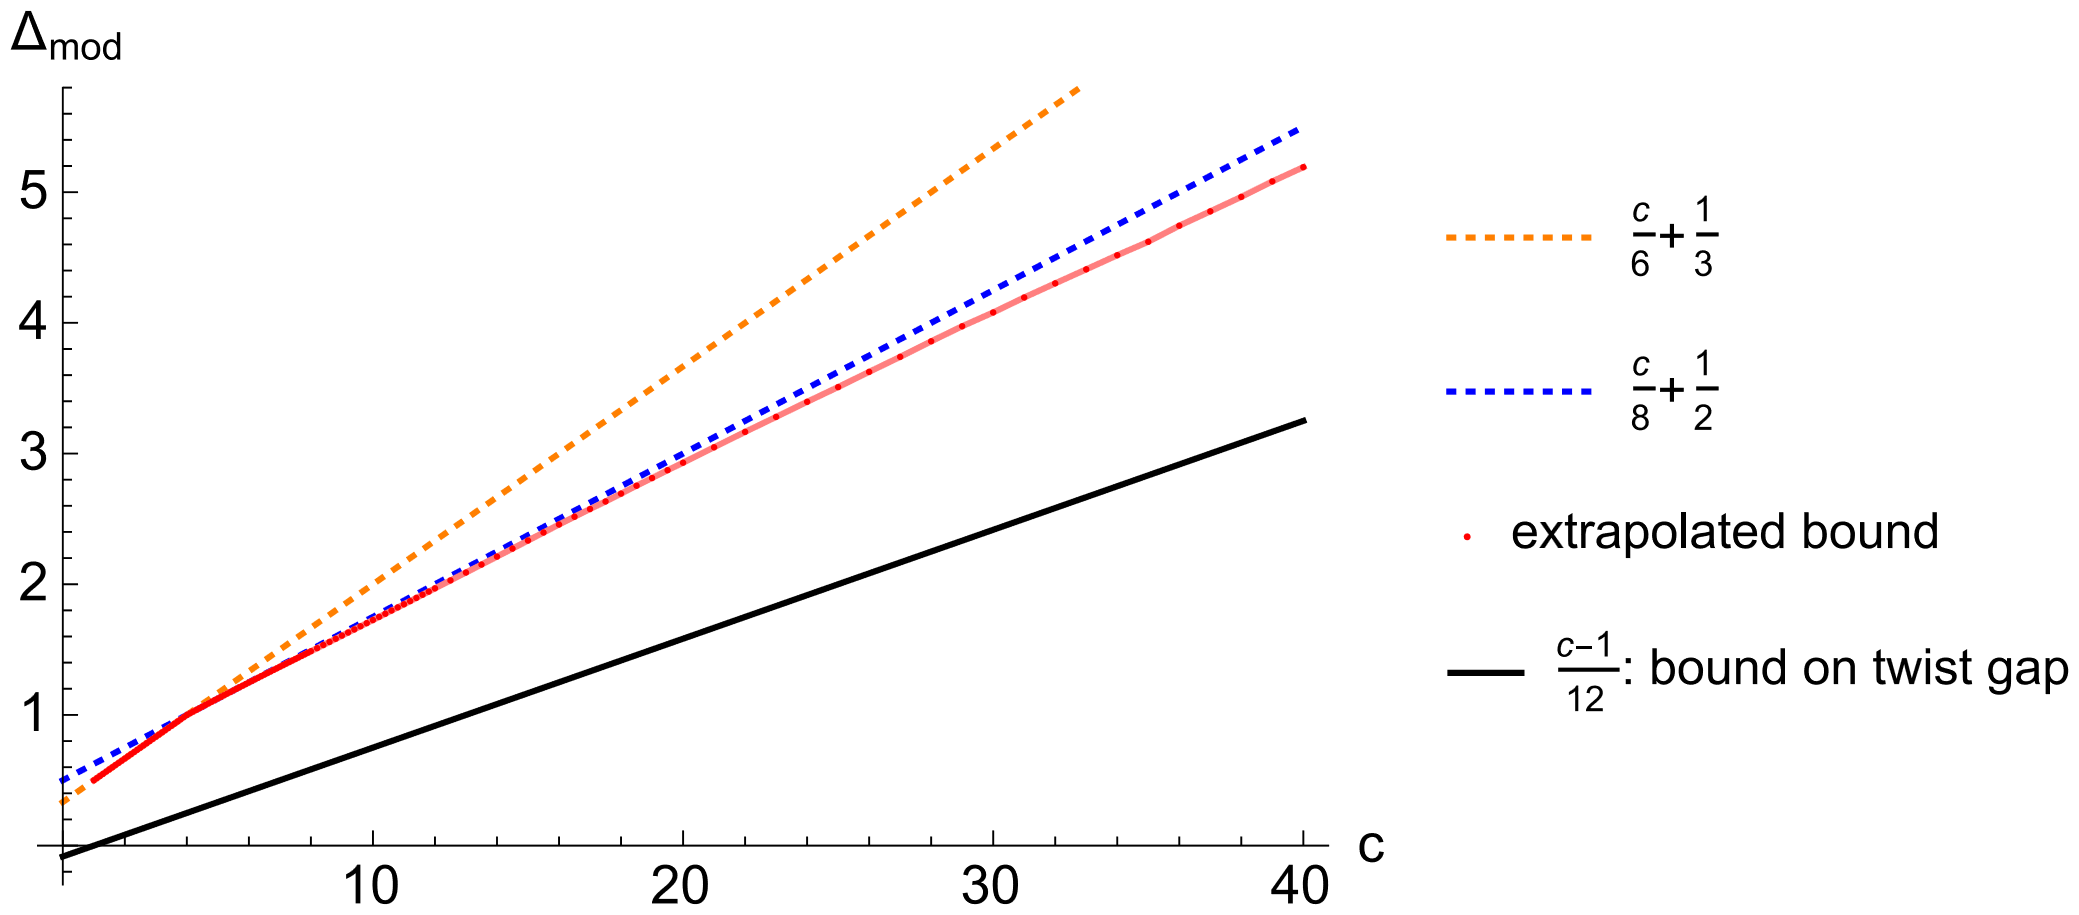
\includegraphics[width=0.85\textwidth]{figures/fig11.png}
  \caption{维数间隙的模界 $\Delta_{\mathrm{mod}}$（红色）作为中心荷 $c$ 的函数，由 $\Delta_{\mathrm{mod}}^{(N)}$ 数值外推到 $N=\infty$ 得到（用 $1/N$ 的二次多项式拟合 $31\le N\le55$ 的结果）\cite{r58}。（原文 p.35，图 11）}
  \label{fig:11}
\end{figure}

可以看到，对 $c\in[1,4]$，$\Delta_{\mathrm{mod}}(c)$ 恰等于 $\frac{c}{6}+\frac13$。它的斜率在 $c=4$ 处从 $\frac16$ 跳到 $\frac18$，此后随 $c$ 光滑、单调地下降。$\Delta_{\mathrm{mod}}(c)$ 严格大于扭曲间隙的上界 $\frac{c-1}{12}$，因此 $\Delta_{\mathrm{mod}}(c)$ 的渐近斜率不小于 $\frac{1}{12}$。$c$ 增大时 $\Delta_{\mathrm{mod}}^{(N)}$ 的收敛变慢；等价地说，决定维数间隙界的最优线性泛函随 $c$ 增大而更多来自 $z,\bar z$ 的高阶导数，这说明导数基在大 $c$ 下效率不高。大 $c$ 极限下最优线性泛函的形式、以及相应的界 $\Delta_{\mathrm{mod}}(c)$，仍是未解问题。
% [Tutor Note: 读图 11 时可对照三条参考线：橙色短虚线是 $c/6+1/3$，蓝色虚线是 $c/8+1/2$，黑实线是扭曲间隙上界 $(c-1)/12$。红点（外推界）在 $c\le4$ 段与橙线完全重合，这是 $\Delta_{\mathrm{mod}}=\frac{c}{6}+\frac13$ 的直接体现；$c>4$ 后红点落到橙线下方，斜率降到 $1/8$ 附近，此后继续平缓减小，于是在 $c$ 很大时红点略低于蓝线。扭曲间隙指谱中 $h-\tilde h$ 的最小非零值，它给出斜率的渐近下界 $1/12$。]

另一个有意思的问题是：束缚紧致幺正 CFT 中第一个非平凡标量 Virasoro 原初场的维数。为此要换一个关于谱的假设：只允许维数为 $\Delta\ge\Delta_0$ 的标量原初场（外加真空），而非零自旋 $s=|h-\tilde h|$ 的原初场权重任意，只要满足幺正性界限 $h,\tilde h\ge0$。此时只要 $c<25$，维数间隙就存在非平凡上界 $\Delta_{\mathrm{mod}}^{s=0}$。数值结果见图~\ref{fig:12}。

\begin{figure}[htbp]
  \centering
  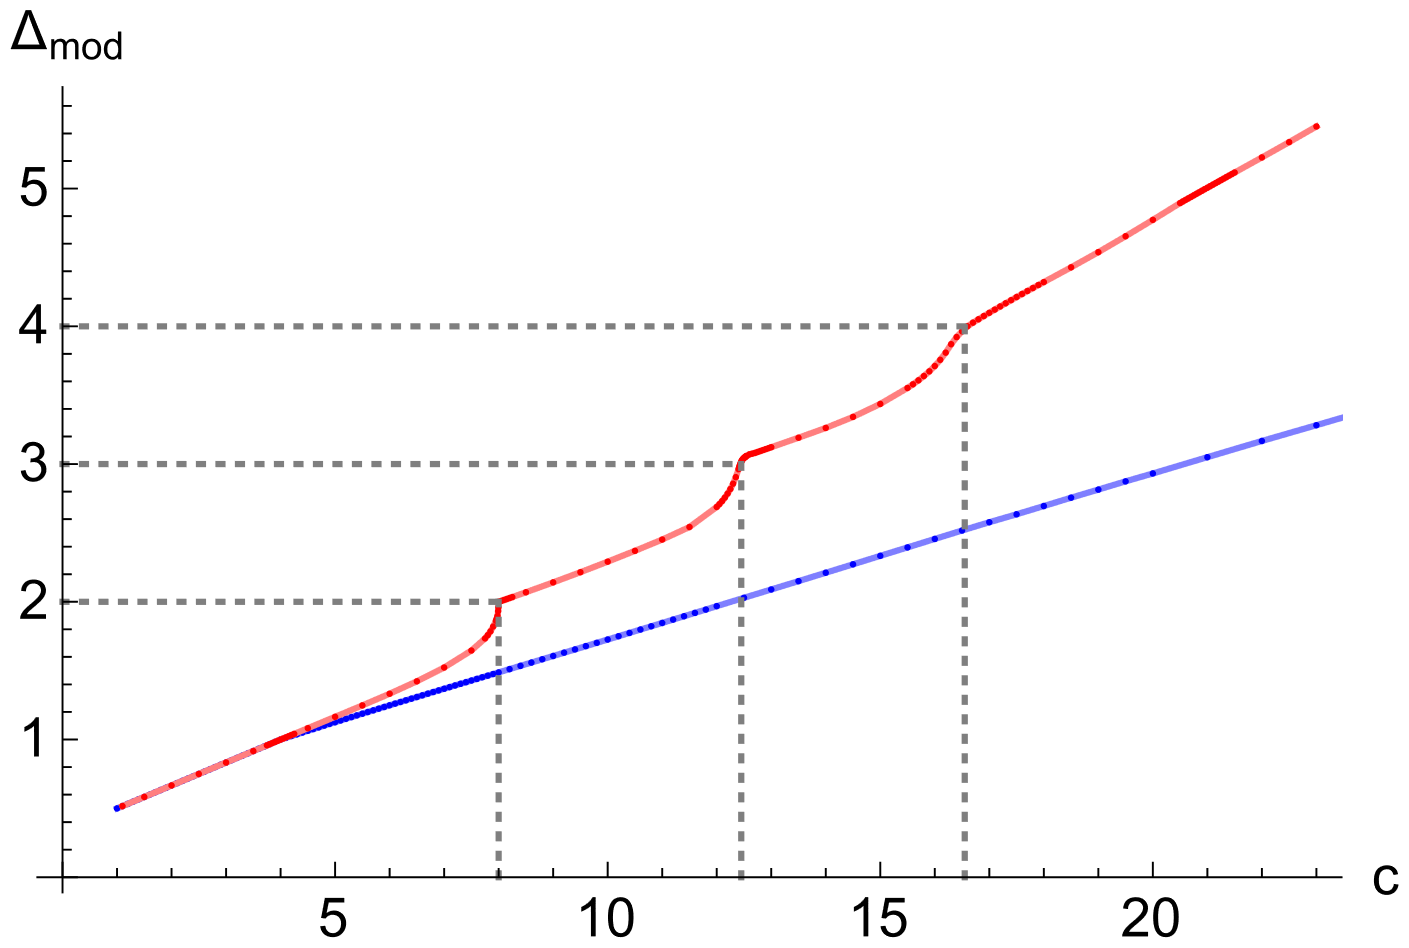
\includegraphics[width=0.85\textwidth]{figures/fig12.png}
  \caption{最轻标量算符维数的模界 $\Delta_{\mathrm{mod}}^{s=0}$（红色）作为中心荷 $c$ 的函数，与全自旋维数间隙界 $\Delta_{\mathrm{mod}}$（蓝色）作比较 \cite{r58}。（原文 p.35，图 12）}
  \label{fig:12}
\end{figure}

按定义，$c\le4$ 时 $\Delta_{\mathrm{mod}}^{s=0}(c)$ 与 $\Delta_{\mathrm{mod}}(c)$ 重合，此处界不超过 $1$。$c>4$ 时 $\Delta_{\mathrm{mod}}^{s=0}(c)$ 严格大于 $\Delta_{\mathrm{mod}}(c)$，并在 $c=25$ 处发散。数值结果还显示出若干有趣特征。界 $\Delta_{\mathrm{mod}}^{s=0}(c)$ 在 $c=8$ 处有一个折点，该处界等于 $2$。这意味着中心荷 $c<8$ 的一切 CFT 都必须含一个非平凡的相关标量 Virasoro 原初场。还可看到，在特殊值 $c=1,2,\frac{14}{5},4,8$ 处，标量间隙界 $\Delta_{\mathrm{mod}}^{s=0}$ 被规范群为 $SU(2)$、$SU(3)$、$G_2$、$SO(8)$、$E_8$ 的能级 $1$ WZW 模型饱和。
% [Tutor Note: $c=8$ 处界等于 $2$ 的物理含义要紧扣“相关”二字：$\Delta_{\mathrm{mod}}^{s=0}<2$ 表示谱中必有标量原初场维数小于 $2$，即相关算符。$c>8$ 后界超过 $2$，就不再强制相关标量存在，故 $c<8$ 的说法是严格的。五个饱和点是 $SU(2)_1$（$c=1$）、$SU(3)_1$（$c=2$）、$(G_2)_1$（$c=\frac{14}{5}$）、$SO(8)_1$（$c=4$）、$(E_8)_1$（$c=8$），它们都是自对偶的能级 $1$ WZW 模型。]

我们也可以束缚间隙处的标量简并度，只需换一个优化问题。考虑形如 \eqref{eq:5-2} 的线性泛函，并作归一化
\begin{equation}
  \label{eq:5-9}
  \alpha[\chi_0\bar\chi_0]=-1 .
\end{equation}
现在对第一个标量原初场 $h=\tilde h=\frac12\Delta_*$，求 $\alpha[\chi_h\bar\chi_{\tilde h}]$ 的极大值，约束为
\begin{equation}
  \label{eq:5-10}
  \begin{aligned}
  &\alpha[\chi_h\bar\chi_{\tilde h}]\ge0,\qquad h=\tilde h\ge\tfrac12\Delta_*,\\
  &\text{or}\quad h\ne\tilde h,\ h,\tilde h\ge0,\ h-\tilde h\in\mathbb{Z} .
  \end{aligned}
\end{equation}
设已找到这样的线性泛函 $\alpha_*$，把它代入模交叉方程，得
\begin{equation}
  \label{eq:5-11}
  \begin{aligned}
  0&=\alpha_*\Bigl[\chi_0\bar\chi_0+d_{\mathrm{gap}}\,\chi_{\frac{\Delta_0}{2}}\bar\chi_{\frac{\Delta_0}{2}}
  +\sum_{\mathrm{rest}}\chi_h\bar\chi_{\tilde h}\Bigr]\\
  &\ge-1+d_{\mathrm{gap}}\,\alpha_*\Bigl[\chi_{\frac{\Delta_0}{2}}\bar\chi_{\frac{\Delta_0}{2}}\Bigr],
  \end{aligned}
\end{equation}
其中 $d_{\mathrm{gap}}$ 是维数 $\Delta_0$ 处的标量简并度。于是 $\bigl(\alpha_*[\chi_{\frac{\Delta_0}{2}}\bar\chi_{\frac{\Delta_0}{2}}]\bigr)^{-1}$ 给出 $d_{\mathrm{gap}}$ 的严格上界。当然，$\Delta_0$ 不应超过 $\Delta_{\mathrm{mod}}^{s=0}$。图~\ref{fig:13} 给出 $\Delta_0=\Delta_{\mathrm{mod}}^{s=0}$ 时 $d_{\mathrm{gap}}$ 的上界在一段 $c$ 范围内的数值结果。

\begin{figure}[htbp]
  \centering
  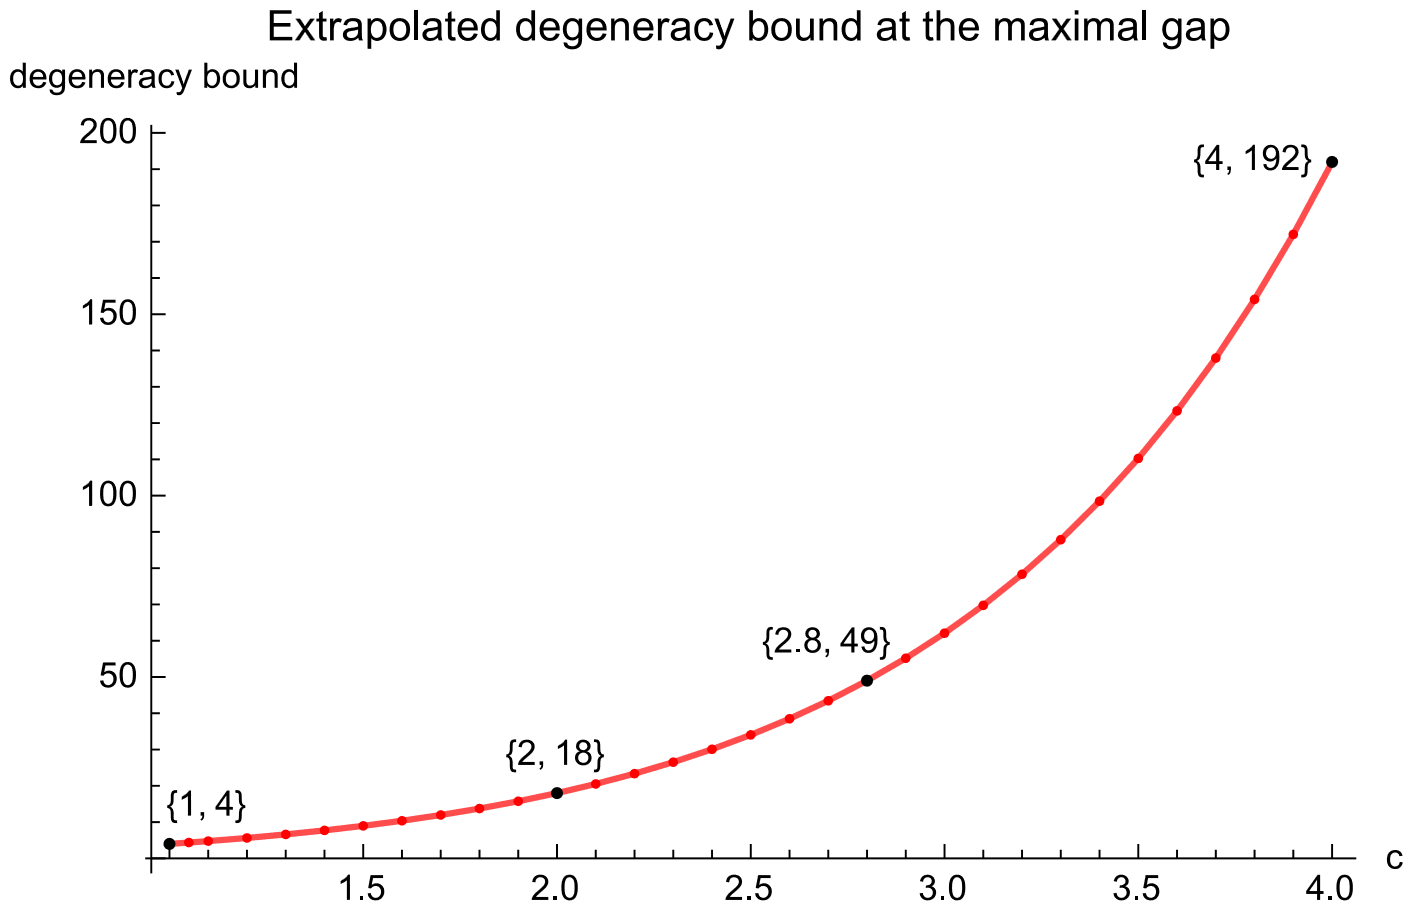
\includegraphics[width=0.85\textwidth]{figures/fig13.png}
  \caption{$\Delta_{\mathrm{mod}}^{s=0}(c)$ 处标量简并度的上界，$1\le c\le4$。黑点对应 $SU(2)_1$、$SU(3)_1$、$(G_2)_1$ 与 $SO(8)_1$ WZW 模型，简并度界在这些点上饱和 \cite{r58}。（原文 p.36，图 13）}
  \label{fig:13}
\end{figure}

\begin{figure}[htbp]
  \centering
  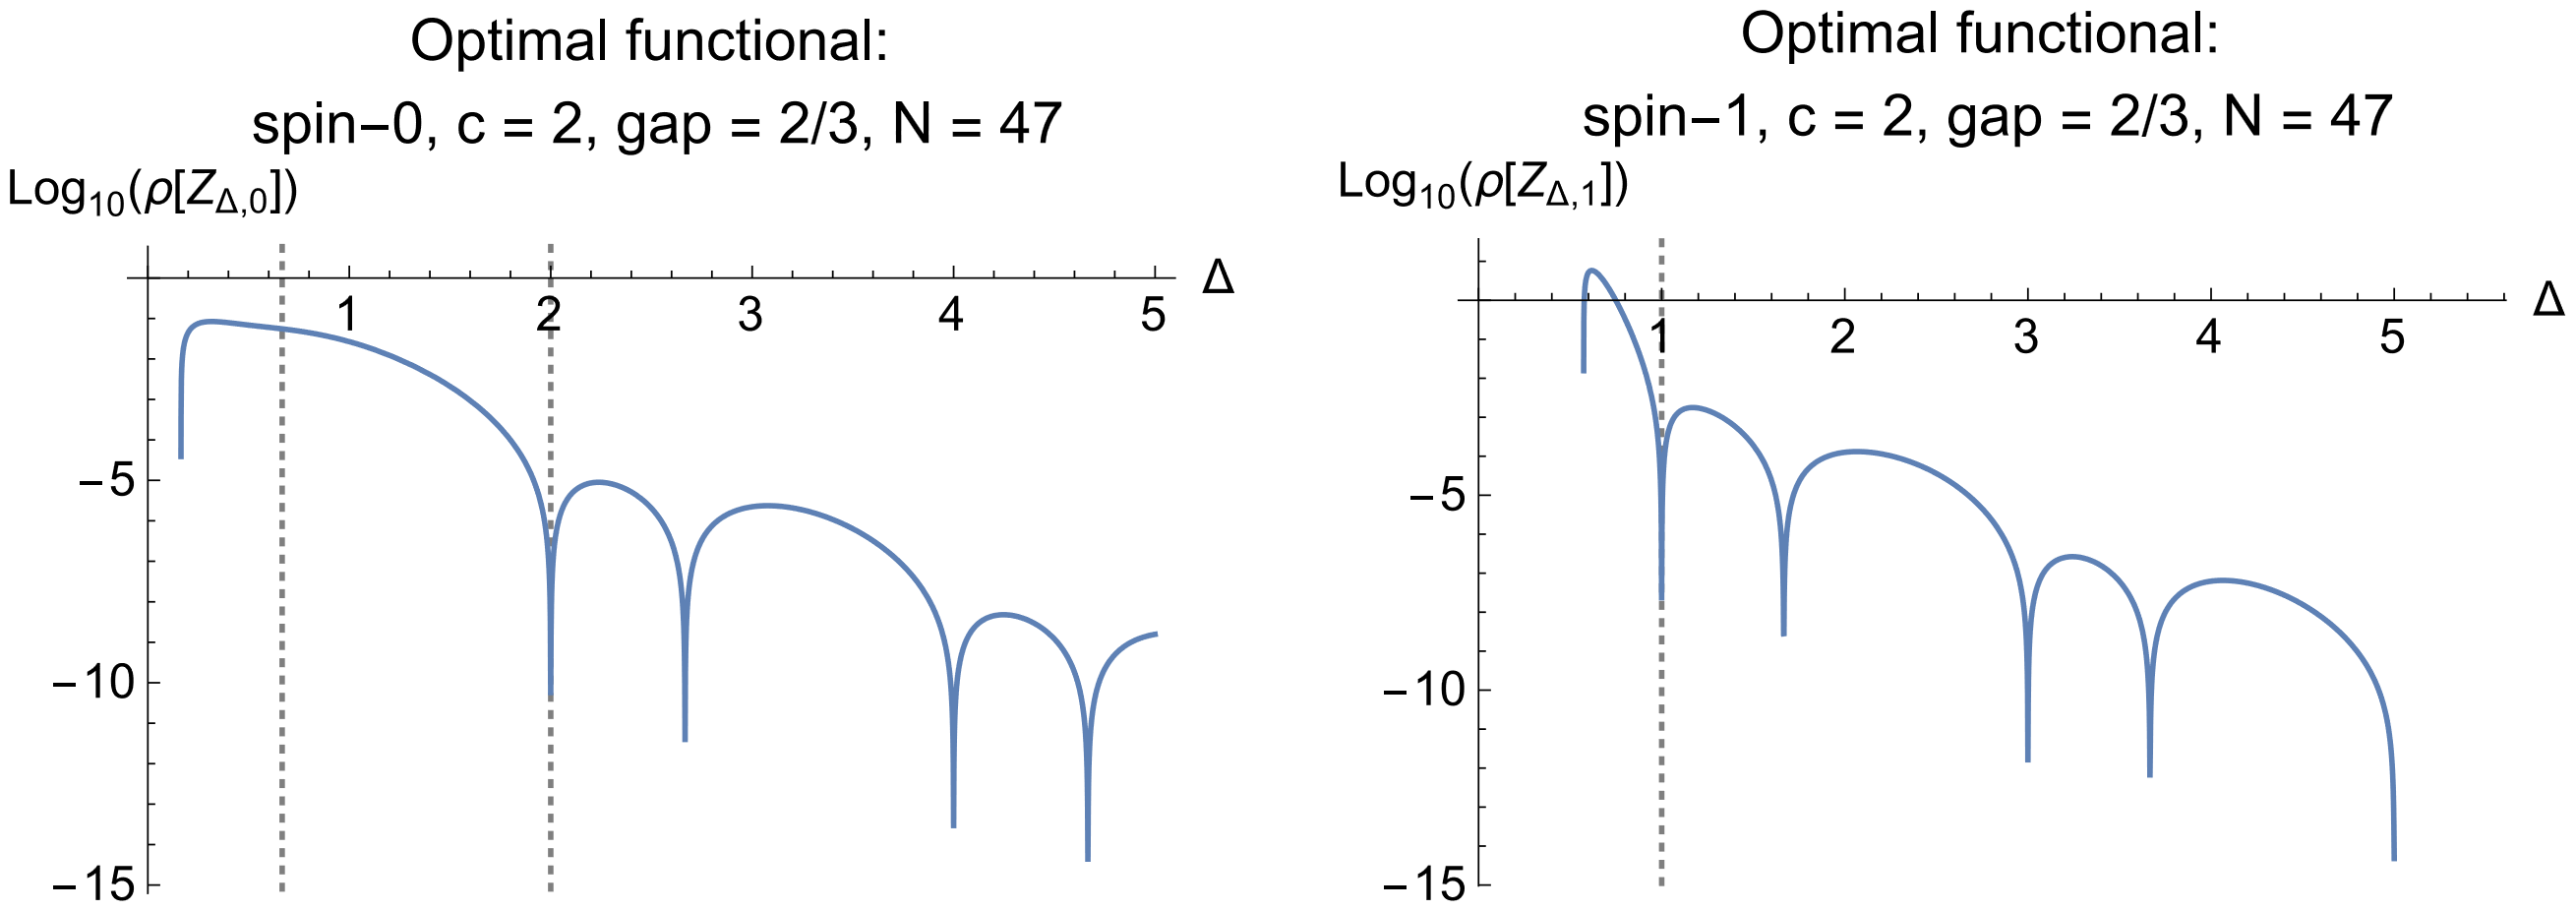
\includegraphics[width=0.85\textwidth]{figures/fig14.png}
  \caption{间隙处算符简并度取极大、且 $c=2$ 处维数间隙界被饱和时，最优泛函作用在自旋 $0$ 与自旋 $1$ 特征标上的对数图。竖直虚线标出间隙，以及自旋 $0$ 情形下的边缘标量原初场与自旋 $1$ 情形下的守恒自旋 $1$ 流 \cite{r58}。（原文 p.36，图 14）}
  \label{fig:14}
\end{figure}
% [Tutor Note: 图 14 两个面板的横轴都是 $\Delta$，纵轴是 $\log_{10}\rho[\cdots]$，即泛函在对应特征标上的取值取对数。读数要点：曲线在每个原初场维数处出现向下的尖峰（即泛函的零点）；左图第二条竖直虚线在 $\Delta=2$，对应边缘标量原初场，右图虚线在 $\Delta=1$，对应守恒自旋 $1$ 流。$c=2$ 的 $SU(3)_1$ 正是标量间隙界与简并度界同时饱和的模型，故其零点位置与 $SU(3)_1$ 的谱结构对应。]

若某个 CFT 恰好饱和了 $d_{\mathrm{gap}}$ 的界，则谱中其余部分的 $(h,\tilde h)$ 必须满足 $\alpha_*[\chi_h\bar\chi_{\tilde h}]=0$。换言之，原初场谱的其余部分落在 $\alpha_*[\chi_h\bar\chi_{\tilde h}]$ 作为 $(h,\tilde h)$ 的函数的零点集内。这就是“极值泛函方法” \cite{r59,r60}。只要某个特征标或共形块展开的系数已知、或被猜想为在所关心的 CFT 上取极大，该方法就能用于各种自举分析。

$c=2$ 的一个例子见图~\ref{fig:14}：使间隙 $\Delta_0=\frac23$ 最大的极值泛函 $\alpha_*$，在自旋 $0$ 与自旋 $1$ 特征标上的零点，与相应自旋的 $SU(3)$ WZW 模型在标量间隙之上的谱吻合。

\subsection{束缚谱函数}\label{sec:5-2}

本节转向谱函数方法。它从交叉方程中提取的不仅是算符谱间隙的界，还包括整个谱上算符贡献的界 \cite{r61}。

设四个全同标量原初场的维数为 $\Delta_\phi$。其四点函数 $g(z,\bar z)=\langle\phi(0)\phi(z,\bar z)\phi(1)\phi'(\infty)\rangle$ 的共形块分解为
\begin{equation}
  \label{eq:5-12}
  g(z,\bar z)=\sum_{h,\tilde h}C^2_{h,\tilde h}\,\mathcal{F}_h(z)\overline{\mathcal{F}}_{\tilde h}(\bar z),
\end{equation}
% [Tutor Note: 原文第四个算符写作 $\phi'(\infty)$，带一撇；按“四个全同标量原初场”的上下文，通常应读作 $\phi(\infty)$。此处照原文排，核对时不必据此改动 $C^2_{h,\tilde h}$ 的定义。]
其中 $C^2_{h,\tilde h}$ 表示 $\phi\phi$ OPE 中权重为 $(h,\tilde h)$ 的原初场的 OPE 系数平方和，$\mathcal{F}_h(z)$ 是内权重为 $h$ 的 Virasoro 共形块（这里略去了对 $\phi$ 的权重与中心荷 $c$ 的显式依赖）。交叉方程取形式
\begin{equation}
  \label{eq:5-13}
  \sum_{h,\tilde h}C^2_{h,\tilde h}\bigl[\mathcal{F}_h(z)\overline{\mathcal{F}}_{\tilde h}(\bar z)
  -\mathcal{F}_h(1-z)\overline{\mathcal{F}}_{\tilde h}(1-\bar z)\bigr]=0,
\end{equation}
或写成 $F^{m,n}(h,\tilde h)\equiv\partial_z^m\partial_{\bar z}^n[\mathcal{F}_h(z)\overline{\mathcal{F}}_{\tilde h}(\bar z)]_{z=\bar z=\frac12}$ 的形式：
\begin{equation}
  \label{eq:5-14}
  \sum_{h,\tilde h}C^2_{h,\tilde h}F^{m,n}(h,\tilde h)=0,\qquad m,n\ge0,\ m+n\ \text{odd} .
\end{equation}
% [Tutor Note: 与 (5.2) 同理，(5.14) 只取 $m+n$ 为奇数的项。设 $u=z-\frac12$，则 $z\to1-z$ 就是 $u\to-u$；交叉方程在 $z=\bar z=\frac12$ 附近作 Taylor 展开时，$\mathcal{F}_h(z)\overline{\mathcal{F}}_{\tilde h}(\bar z)-\mathcal{F}_h(1-z)\overline{\mathcal{F}}_{\tilde h}(1-\bar z)$ 的偶阶项自动抵消，只剩奇数阶。故 $F^{m,n}$ 只需对 $m+n$ 奇数取值。]

注意共形块自身在 $z=\bar z=\frac12$ 处恒为正，即 $F^{0,0}(h,\tilde h)>0$（$h,\tilde h\ge0$）。定义谱函数
\begin{equation}
  \label{eq:5-15}
  f(\Delta_*)=\frac{\sum_{h+\tilde h<\Delta_*}C^2_{h,\tilde h}\,
  \mathcal{F}_h(\frac12)\overline{\mathcal{F}}_{\tilde h}(\frac12)}
  {g(\frac12,\frac12)} .
\end{equation}
按定义，幺正 CFT 中全同算符四点关联函数的谱函数是单调不减的，取值介于 $0$ 与 $1$ 之间。它度量维数不超过 $\Delta_*$ 的算符对关联函数的贡献。

利用交叉方程，可以给出 $f(\Delta_*)$ 作为 $\Delta_*$ 的函数的非平凡上下界。为此考虑不等式
\begin{equation}
  \label{eq:5-16}
  \theta(\Delta_*-\Delta)-y_{0,0}-\sum_{m+n\ \text{odd}}y_{m,n}
  \frac{F^{m,n}(h,\tilde h)}{F^{0,0}(h,\tilde h)}\ge0,
  \qquad\forall (h,\tilde h)\in\mathcal{S},
\end{equation}
其中 $\mathcal{S}$ 是 $\phi\phi$ OPE 中出现算符的假想谱，$y_{m,n}\in\mathbb{R}$。对任一给定的 $\Delta_*$，若能找到一组 $y_{m,n}$，使 \eqref{eq:5-16} 对所有满足 $\mathcal{S}$ 上假设的权重 $(h,\tilde h)$ 同时成立，则用 $C^2_{h,\tilde h}F^{0,0}(h,\tilde h)$ 乘 \eqref{eq:5-16}、对 OPE 中的算符求和，并利用交叉方程，得
\begin{equation}
  \label{eq:5-17}
  \sum_{h,\tilde h}C_{h,\tilde h}\bigl[\Theta(\Delta_*-\Delta)-y_{0,0}\bigr]F^{0,0}(h,\tilde h)
  =g\bigl(\tfrac12,\tfrac12\bigr)\bigl(f(\Delta_*)-y_{0,0}\bigr)\ge0 .
\end{equation}
% [Tutor Note: 原文 (5.17) 的求和号前写的是 $C_{h,\tilde h}$，没有平方。按 (5.12) 与交叉方程的求和权重，这里应为 $C^2_{h,\tilde h}$；否则等号右边无法凑出 $g(\frac12,\frac12)f(\Delta_*)$。此处照原文排，属原文笔误。另外 (5.16) 与 (5.17) 里的小写 $\theta$ 与大写 $\Theta$ 是同一阶梯函数，只是原文大小写不一致。]

于是 $y_{0,0}$ 是 $f(\Delta_*)$ 的严格下界。在 \eqref{eq:5-16} 的约束下极大化 $y_{0,0}$，就得到 $f(\Delta_*)$ 的最优下界。数值上用半正定规划求解；作截断 $m+n\le N$ 后得到谱函数的下界，记作 $f_-^{(N)}(\Delta_*)$。同理，在 \eqref{eq:5-16} 的反向不等式约束下极小化 $y_{0,0}$，得到上界 $f_+^{(N)}(\Delta_*)$。

作为玩具例子，取 $N=1$，即只用一阶导数。若用 $z^{-2h_\phi+h}$ 近似 $\mathcal{F}(h;z)$（有时称作“标度块”），则可写 $F^{1,0}/F^{0,0}\approx2(-2h_\phi+h)$，并推出谱函数的下界
\begin{equation}
  \label{eq:5-18}
  y_{0,0}(x)\approx1-\frac{2\Delta_\phi}{x} .
\end{equation}
这个结果当然只是近似，但与 \eqref{eq:5-16} 给出的精确界定性相似。不过它在权重大时相当弱；我们早已知道，高维原初场的尾部贡献必定指数压低。

\begin{figure}[htbp]
  \centering
  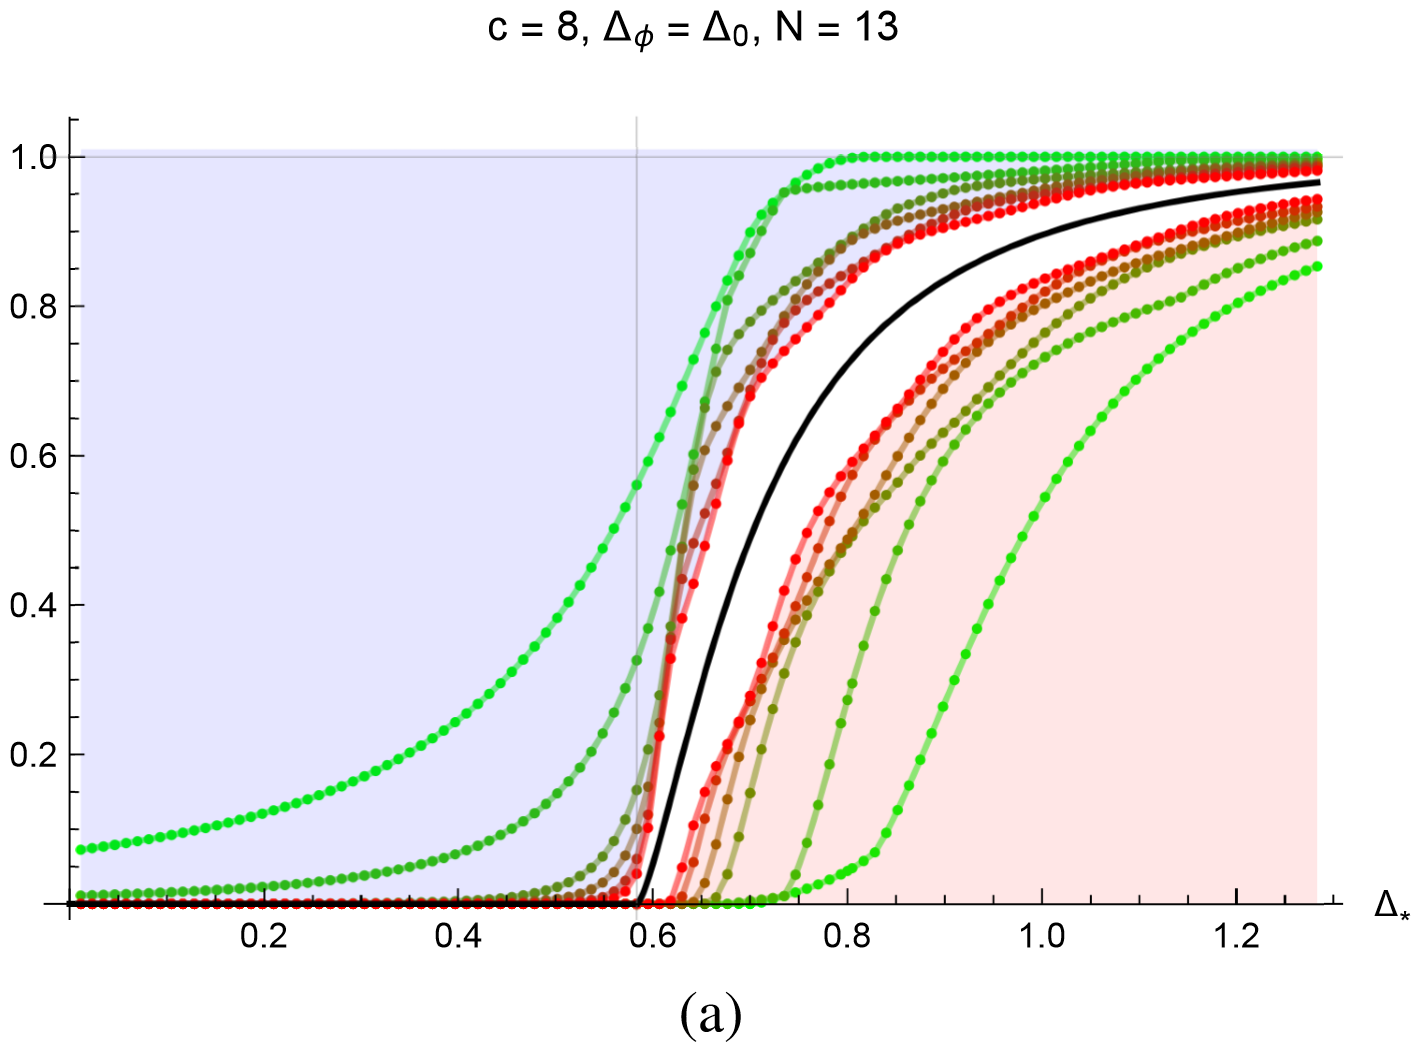
\includegraphics[width=0.85\textwidth]{figures/fig15.png}
  \caption{导数阶 $N$ 递增的线性泛函（由绿到红）给出的谱函数上下界，假设只有标量原初场，取 $c=8$、$\Delta_\phi=\frac{7}{12}$。阴影区被排除，黑线为 Liouville 理论对应的谱函数 \cite{r61}。（原文 p.38，图 15）}
  \label{fig:15}
\end{figure}
% [Tutor Note: (5.18) 里的 $x$ 就是 $\Delta_*$，与 (5.16) 的自变量一致；$1-2\Delta_\phi/x$ 在 $x\gg\Delta_\phi$ 时趋于 $1$，但精确界在 $x\to\infty$ 时会更慢地趋于 $1$。图中绿线到红线对应 $N$ 增大，允许窗口逐级收窄，把黑线（Liouville 谱函数）夹在中间；左侧蓝色与右侧红色阴影区都是被界排除的区域。]

下面考察一个只含标量 Virasoro 原初场（即没有非零自旋原初场）的 $c>1$ 的 CFT 中 $\langle\phi\phi\phi\phi\rangle$ 的谱函数界。我们已经看到，这一假设与模不变性结合，意味着该 CFT 是非紧致的、维数间隙为 $\frac{c-1}{12}$，且其谱密度等于 Liouville CFT 的谱密度。现在若已知谱函数 $f(\Delta_*)$，对 $\Delta_*$ 求导即可还原全部 OPE 系数。

截止到 $N=13$ 的 $f_\pm^{(N)}(\Delta_*)$ 数值结果示例见图~\ref{fig:15}。这些界夹出一个允许的窗口，Liouville 谱函数落在其中。上下界在 $N\to\infty$ 极限下有可能收敛，但数值上难以看出，因为截断阶 $N$ 增高时计算这些界变得非常耗时。

若假定 $N=\infty$ 时上下界重合，就可以直接求解等式
\begin{equation}
  \label{eq:5-19}
  \theta(\Delta_*-\Delta)=y_{0,0}+\sum_{m+n\ \text{odd}}y_{m,n}\,
  \frac{F^{m,n}\bigl(\frac{\Delta}{2},\frac{\Delta}{2}\bigr)}
  {F^{0,0}\bigl(\frac{\Delta}{2},\frac{\Delta}{2}\bigr)},
  \qquad\forall\Delta\ge0 .
\end{equation}
对一切 $\Delta_*\ge0$ 都有解，这等价于 $p_{m,n}(\Delta)=\frac{F^{m,n}(\frac{\Delta}{2},\frac{\Delta}{2})}{F^{0,0}(\frac{\Delta}{2},\frac{\Delta}{2})}$ 作为 $\Delta$ 的函数在正实轴上构成一组完备基，相应的 Hilbert 空间内积为
\begin{equation}
  \label{eq:5-20}
  \langle x,y\rangle=\int_0^\infty x^*(\Delta)\,y(\Delta)\,\mu(\Delta)\,d\Delta ,
\end{equation}
其中 $\mu(\Delta)$ 是某个合适的测度因子。设 $\rho(\Delta)$ 为谱密度，则四点函数在 $z=\bar z=\frac12$ 处的共形块分解取形式 $\int d\Delta\,\rho(\Delta)\,C_\Delta^2F^{0,0}(\frac{\Delta}{2},\frac{\Delta}{2})$。我们想定义矢量 $v(\Delta)=\frac{\rho(\Delta)C_\Delta^2F^{0,0}(\frac{\Delta}{2},\frac{\Delta}{2})}{g(\frac12,\frac12)\mu(\Delta)}$，使之满足
\begin{equation}
  \label{eq:5-21}
  \begin{aligned}
  \langle v,p_{0,0}\rangle&=1,\\
  \langle v,p_{m,n}\rangle&=0,\qquad m,n\ge0,\ m+n\ \text{odd} .
  \end{aligned}
\end{equation}

\begin{figure}[htbp]
  \centering
  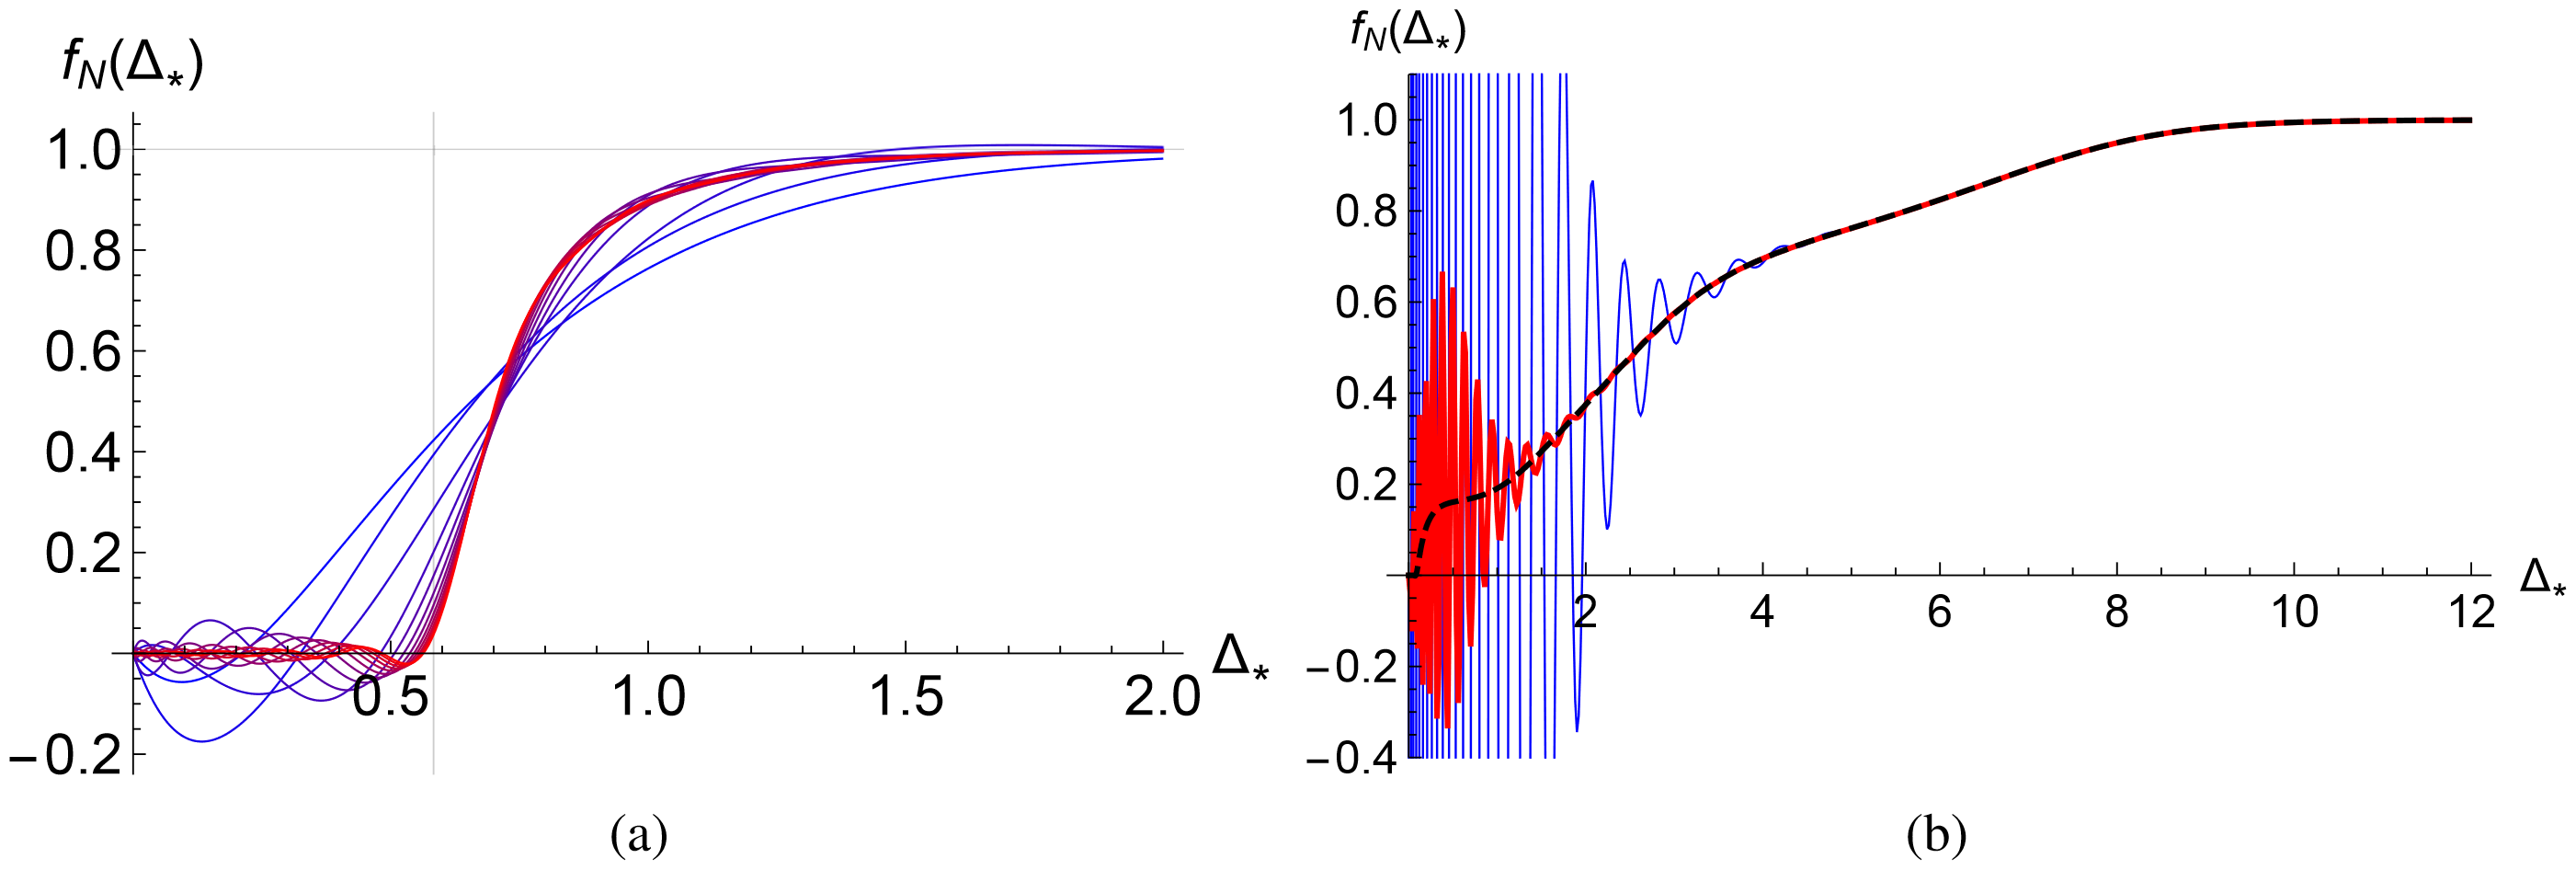
\includegraphics[width=0.85\textwidth]{figures/fig16.png}
  \caption{(a) $c=8$、$\Delta_\phi=\frac{7}{12}$ 时 $f_N(\Delta_*)$ 的图，$N$ 从 $N=1$（蓝）取到 $N=25$（红），步长为 $2$。(b) $c=2$、$\Delta_\phi=\frac{55}{12}$ 时 $f_N(\Delta_*)$（$N=27$ 为蓝色实线，$N=33$ 为红色实线）与精确 DOZZ 谱函数（黑色虚线）的比较。图取自 \cite{r61}。（原文 p.39，图 16）}
  \label{fig:16}
\end{figure}

% [Tutor Note: 原文图 16 (b) 的图注印作 $\Delta_\phi=\frac{55}{12}$（$c=2$）；同图 (a) 的 $7/12=(c-1)/12$，而 $55/12$ 与该关系不符，疑为 $5/12$ 之误或作者另取的参数。译文照原样排，引用该参数时请核对底本。]

测度因子 $\mu(\Delta)$ 的取法应保证内积 $\langle v,v\rangle$ 与 $\langle p_{m,n},p_{m,n}\rangle$ 在 $\Delta$ 上都是收敛积分。回忆 Virasoro 共形块在 $\Delta$ 大时按 $(16q)^\Delta$ 增长（$q$ 为椭圆 nome），OPE 的收敛要求 $\rho(\Delta)C_\Delta^2$ 至少按 $16^{-\Delta}$ 衰减，于是 $\mu(\Delta)v(\Delta)$ 至少按 $e^{-\pi\Delta}$ 衰减。$p_{m,n}(\Delta)$ 按 $\Delta$ 的多项式增长。因此取 $\mu(\Delta)\sim e^{-\lambda\Delta}$，只要 $0<\lambda<2\pi$，即可保证 $\langle v,v\rangle$ 与 $\langle p_{m,n},p_{m,n}\rangle$ 都收敛。实践中取 $\lambda=\pi$。现在取 $v$ 与 \eqref{eq:5-19} 的内积，就得到谱函数
\begin{equation}
  \label{eq:5-22}
  f(\Delta_*)=\langle v,\theta(\Delta_*-\Delta)\rangle .
\end{equation}
% [Tutor Note: 这里省了半步：把 (5.19) 与 $v$ 作内积，右边得 $y_{0,0}\langle v,p_{0,0}\rangle+\sum y_{m,n}\langle v,p_{m,n}\rangle=y_{0,0}$，故 (5.22) 等于说 $y_{0,0}$ 的最优值就是 $f(\Delta_*)$，这正是上下界在 $N=\infty$ 重合的假设所保证的。另注意 $e^{-\pi\Delta}$ 的来源：$z=\bar z=\frac12$ 时椭圆 nome 满足 $q=e^{-\pi K(1-z)/K(z)}=e^{-\pi}$，故 $(16q)^{\Delta}\cdot16^{-\Delta}=e^{-\pi\Delta}$；取 $\lambda<2\pi$ 即要求测度比 $v$ 衰减得更快。]
% [Tutor Note: 补充说明 (5.20) 一式的用意：它把交叉方程的解存在性翻译成函数系 $\{p_{m,n}\}$ 的完备性；原文说“the existence of solution for all $\Delta_*\ge0$ amounts to the completeness”，依据就是 $y_{m,n}$ 与 $\Delta_*$ 无关、而 $\theta(\Delta_*-\Delta)$ 作为 $\Delta$ 的函数必须能在此基下展开。这是标准的矩问题（Hamburger 型）论证。]

% ---------------------------------------------------------------------------
% 本节（5.2）在原书 p.39 末并未结束，续译见后续片段。
% ---------------------------------------------------------------------------


% ============================================================
% Xi Yin, Aspects of Two-Dimensional Conformal Field Theories
%   (PoS(TASI2017)003) 中译片段
% 第 5 章下半：5.2 节续文、5.3 节、5.4 节；第 6 章总结；致谢
% 底本：PDF 第 41--50 页（原书页码 40--49）
% 图 17--21；公式 (5.23)--(5.48)；停止于 References 标题之前
% ============================================================

% ===== 原书 p.40（PDF 41）：5.2 节续文，不重复小节标题 =====

数值上，我们可以用 $P_N v$ 近似 $v$，其中 $P_N$ 是到由 $p_{0,0}$ 与奇 $n+m$ 的 $p_{n,m}$ 张成的子空间上的正交投影。于是，$P_N v$ 可直接由线性方程组
\begin{equation}
  \label{eq:5-23}
  \begin{aligned}
    \langle v_N, p_{0,0}\rangle &= 1,\\
    \langle v_N, p_{m,n}\rangle &= 0,
      \quad m,n\ge 0,\ \text{odd } m+n\le N,
  \end{aligned}
\end{equation}
解出，并得到近似谱函数 $f_N(\Delta_*) = \langle P_N v,\theta(\Delta_*-\Delta)\rangle$。图~\ref{fig:16} 给出两个例子；可以看到 $f_N(\Delta_*)$ 随 $N$ 增大而稳定，并收敛到 Liouville 谱函数。

% [Tutor Note: 段首把基函数写作 $p_{n,m}$，(5.23) 中却写成 $p_{m,n}$；由于条件 $m,n\ge0$ 与奇 $m+n\le N$ 对 $m,n$ 对称，两者指同一族基函数，原文混用不影响线性方程组。]

与形如 $\langle\phi_1\phi_2\bar\phi_2\bar\phi_1\rangle$ 的混合关联子的类似结果一起，数值所提示的“$c>1$ 的 CFT 若只含标量 Virasoro 原初则谱函数唯一”这一性质，将意味着唯一具有该性质的 CFT 是 Liouville 理论。

\begin{figure}[htbp]
  \centering
  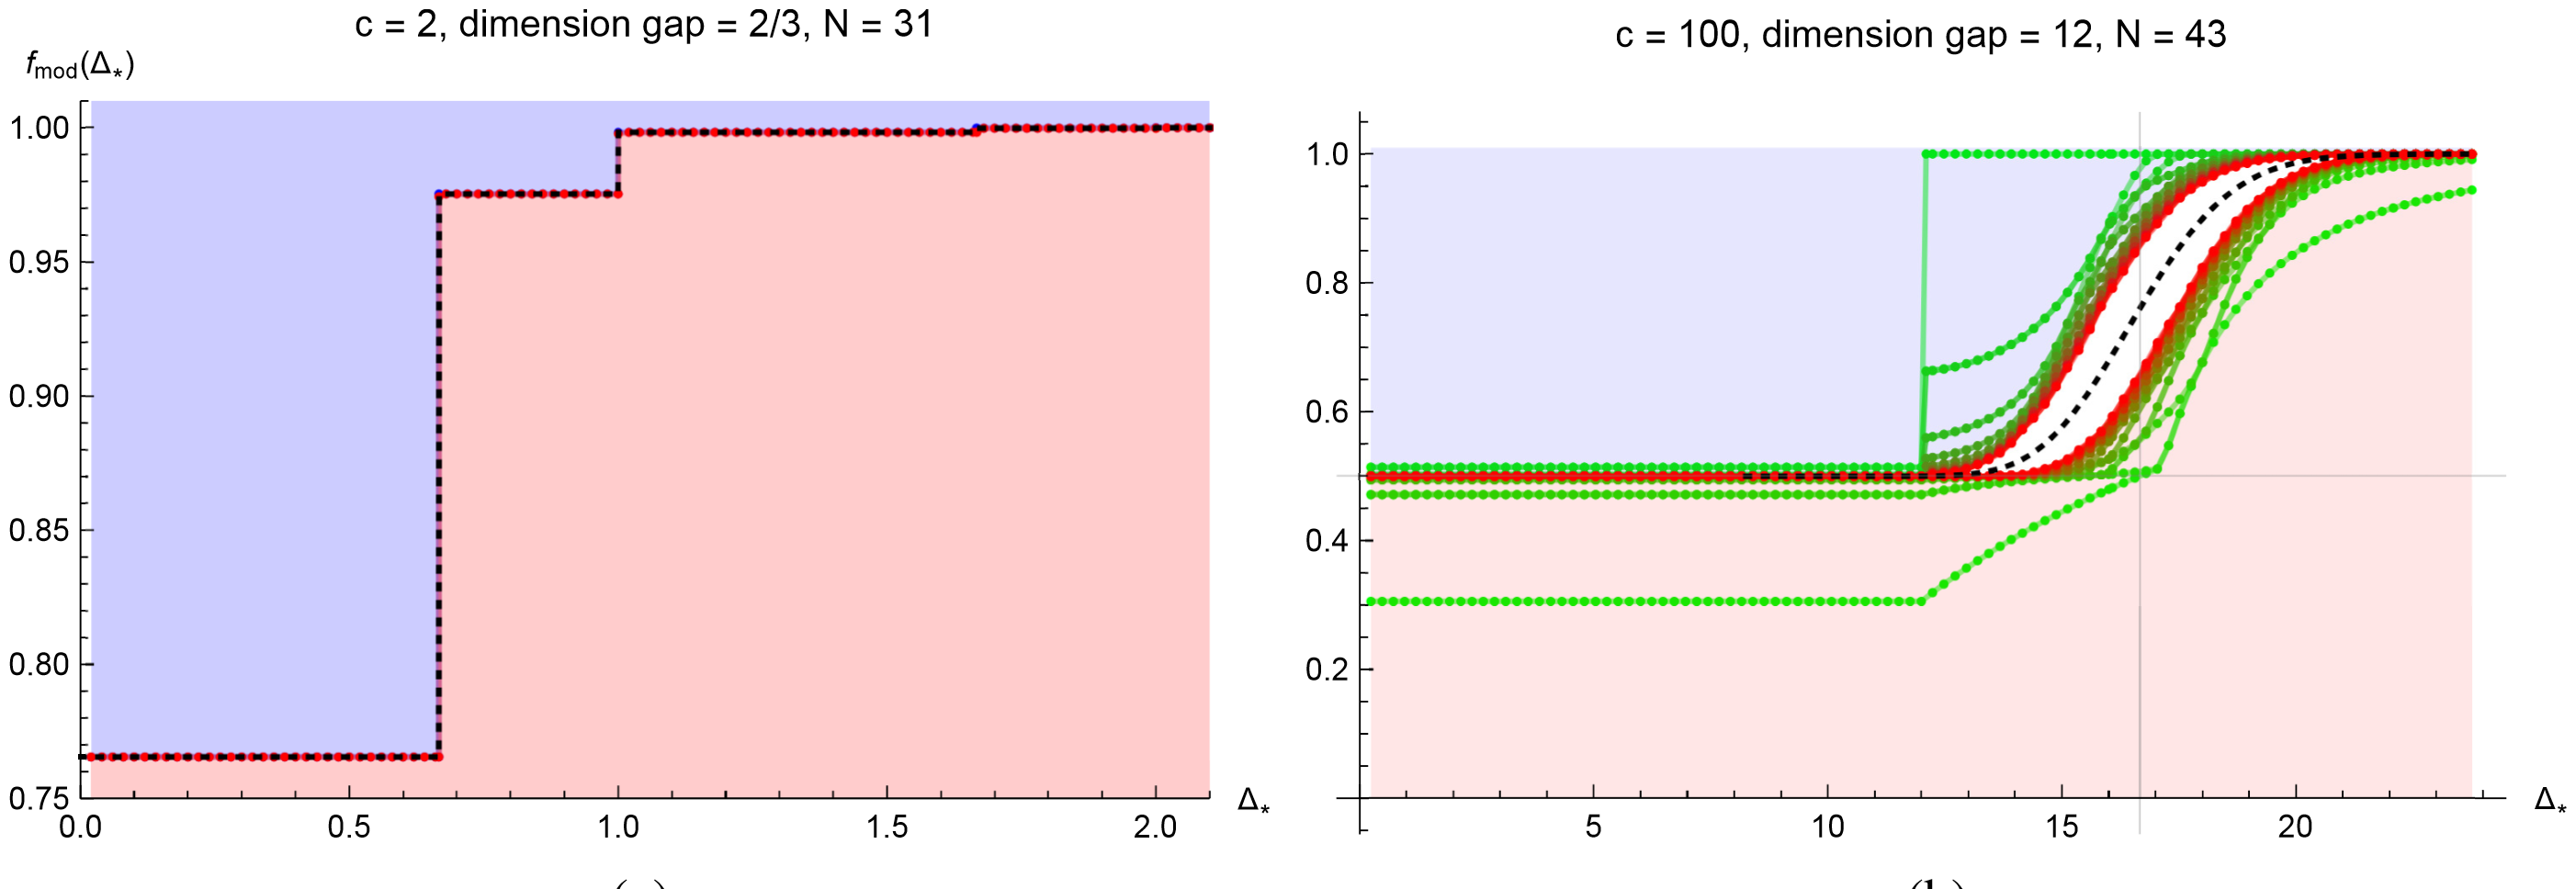
\includegraphics[width=0.85\textwidth]{figures/fig17.png}
  \caption{(a) $c=2$ 时模谱函数的上界（蓝）与下界（红），设间隙等于 $\Delta_{\mathrm{mod}}=\frac23$。(b) $c=100$ 时模谱函数的上、下界，设间隙接近 $\Delta_{\mathrm{mod}}$。黑色虚线是微扰 AdS$_3$ 纯引力的模谱函数，由引力路径积分中的热 AdS$_3$ 鞍点与欧氏 BTZ 鞍点算出。图取自~\cite{r61}。（原文 p.40，图 17）}
  \label{fig:17}
\end{figure}

% [Tutor Note: (5.24) 的分母取 $\tau=-\bar\tau=i$，即 $\tau=i$、$\bar\tau=-i$；$\bar\tau$ 是 $\tau$ 的复共轭，模不变配分函数在自对偶点 $\tau=i$ 的取值正是这样写的，切勿把分母误写成 $Z(\tau=\bar\tau=i)$。]

类似地，我们可以定义模谱函数
\begin{equation}
  \label{eq:5-24}
  f_{\mathrm{mod}}(\Delta_*)
  = \frac{\sum_{h+\tilde h<\Delta_*}\,
      d_{h,\tilde h}\,\chi_h(\tau=i)\,
      \overline{\chi}_{\tilde h}(\bar\tau=-i)}
    {Z(\tau=-\bar\tau=i)},
\end{equation}
并借助模交叉方程、在谱 $\mathcal{S}$ 上作适当假设（比如存在维数间隙 $\Delta_0$）来给它定界。若取 $\Delta_0$ 为维数间隙的模界 $\Delta_{\mathrm{mod}}(c)$，则可期望 $f_{\mathrm{mod}}(\Delta_*)$ 的上、下界收敛并确定谱。实际操作中，用最多 $N$ 阶 $\tau,\bar\tau$ 导数得到的界 $f_{\mathrm{mod},\pm}^{(N)}(\Delta_*)$，在大 $c$ 下随 $N$ 收敛得较慢。

图~\ref{fig:17} 给出模谱函数数值界的两个例子。$c=2$ 时，取最大间隙 $\Delta_{\mathrm{gap}}=\frac23$，界把谱函数确定为 $SU(3)_1$ WZW 模型的谱函数；$c=100$ 时，取接近 $\Delta_{\mathrm{mod}}$ 的间隙，数值界缓慢收敛到 AdS$_3$ 半经典纯引力所预期的答案。

% ===== 原书 p.41（PDF 42）：5.3 节 =====

\subsection{超共形理论的一些结果}\label{sec:5-3}

我们将用两个非平凡的例子，简要介绍超共形场论（SCFT）中关于 BPS 算符 OPE 间隙定界的一些结果。

首先考虑由 K3 上的超对称非线性 sigma 模型定义的 $c=6$ 的 $(4,4)$ SCFT。算符谱可以按小 $\mathcal{N}=4$ 超共形代数（SCA）的表示来组织。在 NS 扇区，表示由超共形原初的权 $h$ 与 $SU(2)_R$ 自旋 $\ell$ 标记。非 BPS 表示 $[h,\ell]$ 满足 $h>\ell$，而 $c=6$ 的 $\mathcal{N}=4$ SCA 中 $SU(2)$ 自旋的允许值只有 $\ell=0$。BPS 表示则满足 $h=\ell$，$\ell$ 可取 $0$ 或 $\frac12$；我们直接把该表示记为 $\langle\ell\rangle$。把手征扇区与反手征扇区合并，得到以下几类表示：
\begin{equation}
  \label{eq:5-25}
  \begin{aligned}
    &\text{vacuum}: \langle 0;0\rangle,\\
    &\tfrac12\text{-BPS}: \langle \tfrac12;\tfrac12\rangle,\\
    &\tfrac14\text{-BPS}: [s,0;\tfrac12\rangle,\
      \langle \tfrac12;s,0],\quad s=1,2,\cdots,\\
    &\text{non-BPS}: [h,0;\tilde h,0],\quad
      h,\tilde h>0,\ h-\tilde h\in\mathbb{Z}.
  \end{aligned}
\end{equation}
% [Tutor Note: (5.25) 用 $(4,4)$ SCA 的表示论组织谱，关键在于 BPS 条件 $h=\ell$：$c=6$ 的小 $\mathcal{N}=4$ 代数中 $SU(2)_R$ 自旋只允许 $0,\frac12$ 的 BPS 值，因此 BPS 原初只分 $\frac12$-BPS 与 $\frac14$-BPS 两类；整理 (5.25) 时勿把 R 自旋 $\ell$ 与共形权 $h$ 混同。]

这里假定工作在共形流形上的一个一般点，即除超共形代数外没有额外守恒流。注意 $\frac14$-BPS 原初有半整数自旋，但其半整数能级的 $\mathcal{N}=4$ 后代自旋为整数，会存活过 GSO 投影。$\frac12$-BPS 与 $\frac14$-BPS 原初的简并度由椭圆亏格决定。结果可总结为如下 BPS 算符内容
\begin{equation}
  \label{eq:5-26}
  \langle 0;0\rangle\oplus 20\langle\tfrac12;\tfrac12\rangle
  \oplus\bigoplus_{s=1}^{\infty} n_s
  \Bigl([s,0;\tfrac12\rangle\oplus\langle\tfrac12;s,0]\Bigr),
\end{equation}
其中 $n_1=90$、$n_2=462$、$n_3=1540$，等等。$20$ 个 $\frac12$-BPS 表示给出 $80$ 个保持 $(4,4)$ SCA 的精确边缘形变，它们对应共形流形
\[
  \mathcal{M}\simeq
  \mathrm{Aut}(\Gamma_{20,4})\backslash SO(20,4)/
  \bigl(SO(20)\times SO(4)\bigr)
\]
的切方向。

% [Tutor Note: $20$ 个 $\frac12$-BPS 表示给出 $80=20\times4$ 个精确边缘形变，而陪集 $\mathrm{Aut}(\Gamma_{20,4})\backslash SO(20,4)/(SO(20)\times SO(4))$ 在一般点的切空间维数正是 $20\times4=80$；这个计数是检验“边缘形变数目”与“模空间维数”是否一致的快速办法。]

尽管 BPS 算符谱沿共形流形 $\mathcal{M}$ 不变（例外是某些特殊点：那里有些非 BPS 原初变成 BPS，并给出额外的守恒高自旋流），非 BPS 算符谱却对精确边缘形变有高度非平凡的依赖。共形流形 $\mathcal{M}$ 可等价地描述为嵌入 $\mathbb{R}^{20,4}$ 的 Narain 格 $\Gamma_{20,4}$ 的模空间。格矢量 $\ell\in\Gamma_{20,4}$ 可按其在 $\mathbb{R}^{20,4}$ 正、负子空间上的投影分解，记为 $(\ell_L,\ell_R)$。只要格的嵌入使某个满足 $\ell^2\equiv\ell_L^2-\ell_R^2=2$ 的格矢量落在正子空间内，即 $\ell_R=0$，模空间中的对应点就给出奇异的 K3 CFT：该 CFT 在某个维数间隙之上发展出连续谱。这类奇点有 ADE 分类，与 IIA 型弦论紧化在 K3 上时六维规范对称性的增强有关。

抓住 K3 CFT 模依赖的一个精确结果如下~\cite{r62,r63}。设 $\phi_i^{\pm,\pm}$ 是 $\frac12$-BPS 的 (NS,NS) 原初，它们在手征与反手征 $SU(2)$ R 对称性的二重态中变换。经半单位谱流，它联系到 (R,R) 原初 $\phi_i^{RR}$，

% ===== 原书 p.42（PDF 43）=====

后者是 R 对称性的单态，共形权为 $(\frac14,\frac14)$。现在考虑积分四点函数
\begin{equation}
  \label{eq:5-27}
  \begin{aligned}
    &\int d^2z\,|z|^{-s-1}|1-z|^{-t-1}
    \bigl\langle \phi_i^{RR}(0)\phi_i^{RR}(z,\bar z)
      \phi_k^{RR}(1)\phi_\ell^{RR'}(\infty)\bigr\rangle\\
    &\quad = 2\pi\left(
      \frac{\delta_{ij}\delta_{k\ell}}{s}
      + \frac{\delta_{i\ell}\delta_{ij}}{t}
      + \frac{\delta_{ik}\delta_{j\ell}}{u}\right)
      + A_{ijk\ell} + B_{ij,k\ell}\,s
      + B_{i\ell,kj}\,t + B_{ik,j\ell}\,u
      + O(s^2,t^2,u^2),
  \end{aligned}
\end{equation}
其中 $u\equiv -s-t$，左端由 $s,t$ 的适当区域解析延拓定义（在该区域积分收敛）；也可以从 $z$ 的被积函数中减去适当的抵消项，直接在 $s=t=0$ 附近展开积分。在 IIB 型弦论紧化于 K3 的语境中，\eqref{eq:5-27} 可解释为六维四个张量多重态的弦树图级散射振幅。利用超对称性，由六维 $(2,0)$ 超引力的超振幅分析得到的非重整化结果（此处不回顾），可以把系数 $A_{ijk\ell}$ 与 $B_{ij,k\ell}$ 确定为 K3 CFT 共形流形上的精确函数。

% [Tutor Note: 原文 (5.27) 有两处疑似笔误：左端第二个算符写作 $\phi_i^{RR}$，按右端系数 $A_{ijk\ell}$、$B_{ij,k\ell}$ 的指标结构应为 $\phi_j^{RR}$；$t$ 道交叉项的分子写作 $\delta_{i\ell}\delta_{ij}$，按 $s,t,u$ 三道的置换对称性应为 $\delta_{i\ell}\delta_{jk}$。译文照原文排，以便与底本逐符号对照。]

% [Tutor Note: 原文在四点函数的第四个算符上一律加撇（本式为 $\phi_\ell^{RR'}$，后文 (5.31) 为 $\phi_1^{RR'}$、(5.32) 为 $\phi^{-,-'}$、(5.44) 为 $\bar\sigma_3'$），而正文叙述中同一算符不带撇；疑为原文排版或记号习惯，译文保留原样。]

例如 $A_{ijk\ell}$ 由
\begin{equation}
  \label{eq:5-28}
  A_{ijk\ell}
  = \frac{1}{16\pi^2}\,
    \frac{\partial^4}{\partial y^i\partial y^j\partial y^k\partial y^\ell}
    \bigg|_{y=0}
    \int_{\mathcal{F}} d^2\tau\,
    \frac{\Theta_\Lambda(y|\tau,\bar\tau)}{(\eta(\tau))^{24}},
\end{equation}
给出，其中 $\mathcal{F}$ 是 $PSL(2,\mathbb{Z})$ 作用在上半平面上的基本区域，$\Lambda$ 表示嵌入 $\mathbb{R}^{20,4}$ 的格 $\Gamma_{20,4}$，它参数化 K3 CFT 共形流形上的一点。格 theta 函数 $\Theta_\Lambda$ 定义为
\begin{equation}
  \label{eq:5-29}
  \Theta_\Lambda(y|\tau,\bar\tau)
  = e^{\frac{\pi}{2\tau_2}y^2}
    \sum_{\ell\in\Lambda}
    e^{i\pi\tau\ell_L^2 - i\pi\bar\tau\ell_R^2
      + 2\pi i\,\ell_L\cdot y}.
\end{equation}
辅助矢量 $y$ 位于正子空间 $\mathbb{R}^{20}$，其分量与 K3 CFT 的 $20$ 个 $\frac12$-BPS 多重态对应。公式~\eqref{eq:5-28} 可从杂化弦/II 型对偶理解为杂化弦单圈振幅，因此要对环面的模积分。$B_{ij,k\ell}$ 有类似的公式，是对亏格二黎曼面模的积分。

% [Tutor Note: (5.29) 中 $\ell_L^2$ 与 $\ell_R^2$ 的系数分别是 $+i\pi\tau$ 与 $-i\pi\bar\tau$，$\bar\tau$ 前的负号最易漏；归一化因子里的 $\tau_2$ 指 $\mathrm{Im}\,\tau$，不要写成 $\bar\tau$。]

% [Tutor Note: (5.28) 的四阶导数在 $y=0$ 取值，而 $y$ 只跑正子空间 $\mathbb{R}^{20}$ 的 $20$ 个分量；$\Theta_\Lambda$ 对 $y$ 的依赖为 $e^{\frac{\pi}{2\tau_2}y^2+2\pi i\ell_L\cdot y}$，逐次求导时高斯因子同样贡献项，不要只对 $e^{2\pi i\ell_L\cdot y}$ 求导。]

我们只用单个原初（比如 $\phi_1^{RR}$）的积分四点函数，即 $A_{1111}$。结果 $A_{1111}$ 取非负实值，并在两种不同极限下发散：(1) 满足 $\ell^2=2$ 的格矢量落在正子空间内，对应 K3 出现 $A_1$ 奇点；或 (2) 零格矢量（即 $\ell_L^2=\ell_R^2$）有 $\ell_L^2,\ell_R^2\to0$，对应 K3 曲面的大体积极限。我们希望把 $\phi_1^{RR}\phi_1^{RR}$ OPE 的非 BPS 算符内容约束为 $A_{1111}$ 的函数，后者编码了对共形流形的依赖~\cite{r64}。

为继续，需要把 $\frac12$-BPS 四点函数按 $(4,4)$ SCA 的超 Virasoro 共形块分解。对 Ward 恒等式作简单分析即可看出：一对 $\frac12$-BPS 原初的 OPE 中可能出现的表示，只有真空/单位表示与非 BPS 表示（后者的 $SU(2)_R$ 自旋必为零）。

% ===== 原书 p.43（PDF 44）=====

BPS 关联子 $\langle\phi^R(0)\phi^R(z)\phi^R(1)\phi^{R'}(\infty)\rangle$（外部算符为 R 扇区中权 $\frac14$ 的算符）在标号为 $[h,0]$ 的非 BPS 道中的手征 $c=6$ $\mathcal{N}=4$ 超共形块，等于外权为 $1$、内权为 $h+1$ 的 $c=28$ 玻色 Virasoro 块，二者只相差一个简单的前因子：
\begin{equation}
  \label{eq:5-30}
  \mathcal{F}_h^{\mathcal{N}=4,R}(z)
  = z^{\frac12}(1-z)^{\frac12}\,
    \mathcal{F}_{c=28}^{\text{Virasoro}}(1,1,1,1,h+1;z).
\end{equation}
这个简单关系成立的原因是：(1) $c=6$ 的 $\mathcal{N}=4$ 超共形块恰好与 $\mathcal{N}=2$ 子代数的对应块重合（$c\ge 12$ 时并非如此）；(2) 含外部 BPS 算符的 $\mathcal{N}=2$ 块与 Virasoro 共形块以简单方式相联系，这可以通过研究 $\mathcal{N}=2$ cigar CFT 的关联子来论证。真空道块可由~\eqref{eq:5-30} 的 $h\to0$ 极限得到。

% [Tutor Note: 注意 (5.30) 的玻色块内权是 $h+1$：$h$ 是 $\mathcal{N}=4$ 超共形权，并非 $c=28$ Virasoro 块的内权；真空道（$h\to0$）对应的是内权为 $1$ 的玻色块，勿直接把内权也取成 $h$。]

\begin{figure}[htbp]
  \centering
  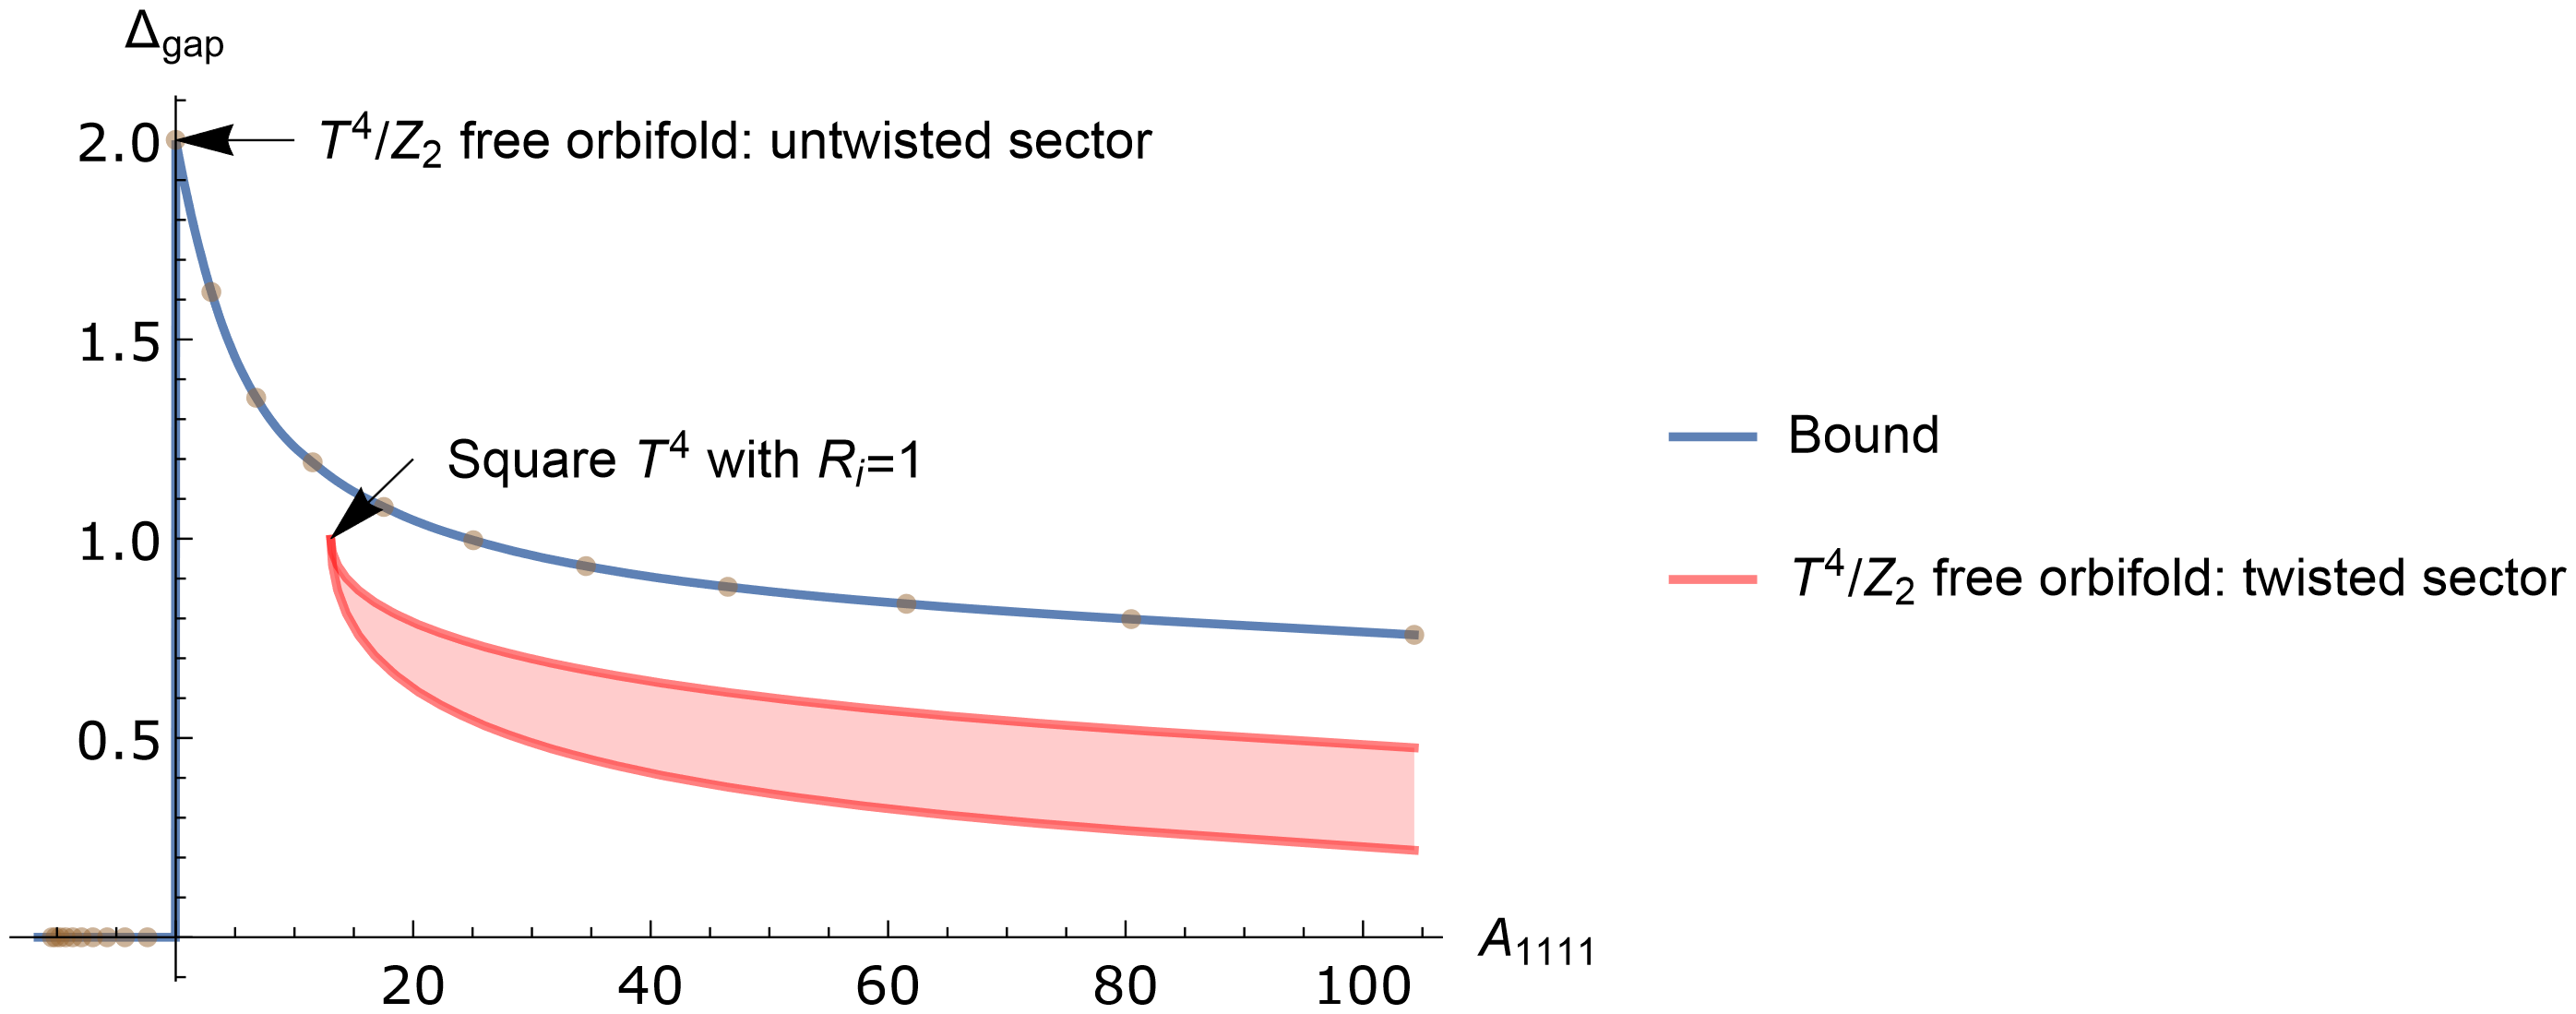
\includegraphics[width=0.85\textwidth]{figures/fig18.png}
  \caption{实心蓝线给出 $\phi_1\phi_1$ OPE 中非 BPS 原初间隙的上界，横轴是积分 BPS 四点函数 $A_{1111}$（橙色圆点是数值数据点，它们在 $20$ 阶导数处已经稳定）。红色阴影区域表示 $T^4/\mathbb{Z}_2$ 某个不动点处 $\frac12$-BPS 扭曲场 OPE 中的间隙，该不动点处 $T^4$ 为矩形。图取自~\cite{r64}。（原文 p.43，图 18）}
  \label{fig:18}
\end{figure}

现在，我们直接对关联子
\begin{equation}
  \label{eq:5-31}
  \bigl\langle \phi_1^{RR}(0)\phi_1^{RR}(z,\bar z)
    \phi_1^{RR}(1)\phi_1^{RR'}(\infty)\bigr\rangle
  = \sum_{h,\tilde h} C_{h,\tilde h}^2\,
    \mathcal{F}_h^{\mathcal{N}=4,R}(z)\,
    \overline{\mathcal{F}}_{h}^{\mathcal{N}=4,R}(\bar z).
\end{equation}
% [Tutor Note: (5.31) 右端第二个块的下标，原文印刷为不带波浪的 $h$（与求和的 $h,\tilde h$ 不一致），译文照原样保留。此处按右移权记作 $\tilde h$ 才是通常的分解，属原文疑似笔误。]
施加交叉方程的约束。来自 $A_{1111}$ 的约束可简单地表述为对 $C_{h,\tilde h}^2$ 的一条额外线性关系，它与交叉方程处于同等地位。分析细节太长，此处不再复述；我们直接把 $\phi_1\phi_1$ OPE 中第一个非 BPS 原初维数间隙上界的结果总结在图~\ref{fig:18} 中。

% [Tutor Note: (5.31) 把交叉方程写成正系数 $C_{h,\tilde h}^2$ 的线性组合，这正是能化为半正定规划的标准形式；对照后面 (5.33) 的结构常数 $C_{ijj}$ 没有先验正性，环面一点函数的模协变约束便难以直接用同一数值方法处理，这是作者在 5.4 节转向亏格二配分函数的动机之一。]

在 $A_{1111}\to\infty$ 极限下，维数间隙界的渐近值从图~\ref{fig:18} 的绘图范围看不出，但数值上求得为 $\Delta_{\mathrm{gap}}=\frac14$。这个值实际上被 $\mathcal{N}=4$ 的 $A_1$ cigar CFT 饱和；该理论有精确描述，即超对称的 $SL(2,\mathbb{R})_2/U(1)$ 陪集，并被猜想能刻画 K3 CFT 出现 $A_1$ 奇点时的奇异极限。

另一个例子我们只作极简讨论：$c=9$ 的 $(2,2)$ SCFT 中 $\frac12$-BPS 算符 OPE 内容的约束~\cite{r65}。这类理论包括 Calabi--Yau 三维流形上的超对称非线性 sigma 模型。如前所述，后者有扩充的 $\mathcal{N}=2$ SCA，这对 BPS 算符的三点函数给出高度非平凡的约束。

% ===== 原书 p.44（PDF 45）=====

在某些情形，比如五次三维流形上的 NLSM，诸如 (chiral, chiral) $\frac12$-BPS 算符的三点函数已被确定为共形流形上的精确函数。这使我们能通过 BPS 算符的 OPE 系数，把模依赖纳入 $\frac12$-BPS 四点函数的分析，从而用交叉方程约束 OPE 的非 BPS 算符内容。

令 $\phi^{+,+}$ 是权为 $(\frac12,\frac12)$ 的 (chiral, chiral) 原初，$\phi^{-,-}$ 是其共轭的 (anti-chiral, anti-chiral) 原初。我们可以按 $\phi^{+,+}\phi^{+,+}$ OPE 道（CC）与 $\phi^{+,+}\phi^{-,-}$ OPE 道（CA）中的 $\mathcal{N}=2$ 超共形块分解来分析四点函数
\begin{equation}
  \label{eq:5-32}
  \bigl\langle \phi^{+,+}(0)\phi^{-,-}(z,\bar z)
    \phi^{+,+}(1)\phi^{-,-'}(\infty)\bigr\rangle,
\end{equation}
并利用 $z\to1-z$ 交叉方程同时约束两个道中第一个非 BPS 原初的间隙。

模依赖可通过 $\phi^{+,+}\phi^{+,+}$ OPE 中一个 R 荷为 $(2,2)$ 的 BPS 原初的 OPE 系数 $\lambda$ 纳入。图~\ref{fig:19} 给出 CC 对 CA 道中非 BPS 谱间隙数值界随 $\lambda$ 变化的一个例子，施用于五次三维流形模型；其中 $\phi^{+,+}$ 是与 Kähler 形变相联系的 BPS 原初，BPS OPE 系数 $\lambda$ 是 Kähler 模空间上的已知函数。可以看到，边界曲面上有些点由自由理论的 OPE 饱和。

\begin{figure}[htbp]
  \centering
  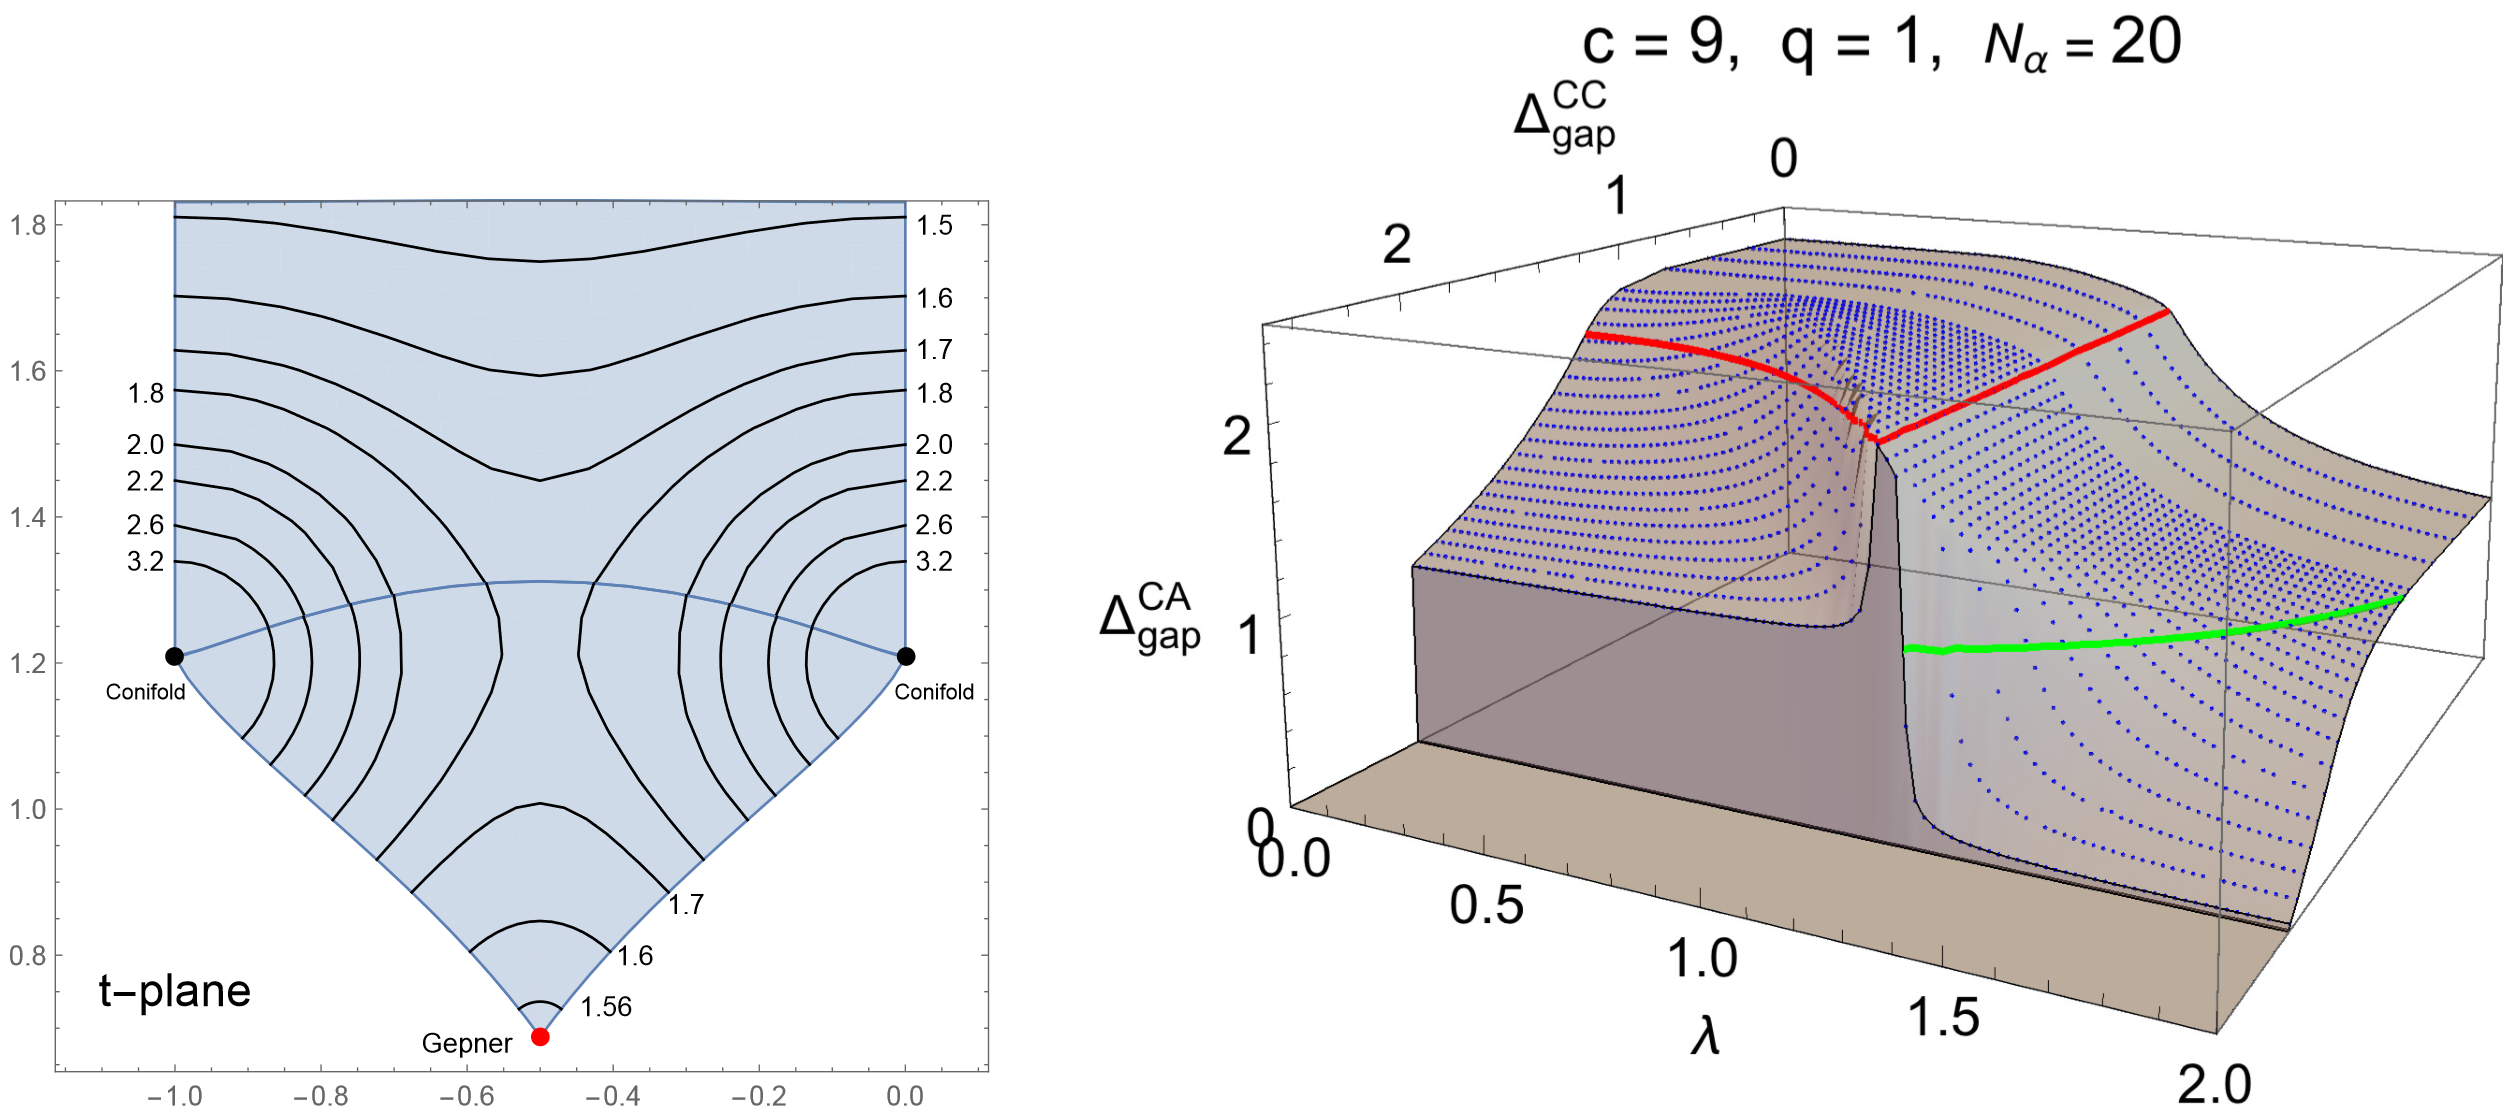
\includegraphics[width=0.85\textwidth]{figures/fig19.png}
  \caption{左：五次三维流形 Kähler 模空间上手征环系数 $\lambda$ 的等值线图~\cite{r66}。黑曲线是 $\lambda$ 的等值线；conifold 点用黑点标出，Gepner 点用红色标出。右：CA 道中间隙 $\Delta_{\mathrm{gap}}^{CA}$ 作为 $\Delta_{\mathrm{gap}}^{CC}$ 与 $\lambda$ 的函数的上界，用最多 $20$ 阶导数的线性泛函算出。$\Delta_{\mathrm{gap}}^{CC}=2$ 截面上的窄峰，预计在导数阶数趋于无穷时收缩为零宽度。图取自~\cite{r65}。（原文 p.44，图 19）}
  \label{fig:19}
\end{figure}

% [Tutor Note: CC 道指 $\phi^{+,+}\phi^{+,+}$ OPE，CA 道指 $\phi^{+,+}\phi^{-,-}$ OPE；$z\to1-z$ 交叉方程把两个道的间隙联系起来。图 19 右图的边界曲面同时约束两个道的间隙，纵轴是 $\Delta^{CA}_{\mathrm{gap}}$，不要把 $\Delta^{CC}_{\mathrm{gap}}$ 也当成纵轴。]

% ===== 原书 p.44 末（PDF 45）：5.4 节开始 =====

\subsection{亏格二模自举}\label{sec:5-4}

到目前为止，我们分析了交叉对称性对单个 OPE 的约束，以及配分函数的模不变性对谱的约束。可以把后者推广到环面一点函数的模协变性。

% ===== 原书 p.45（PDF 46）=====

事实上，把原初 $\phi_i(z,\bar z)$ 的环面一点函数按环面一点 Virasoro 共形块分解，
\begin{equation}
  \label{eq:5-33}
  \bigl\langle \phi_i(z,\bar z)\bigr\rangle_{T^2(\tau)}
  = \sum_j C_{ijj}\,
    \mathcal{F}_c^{T^2}(h_i,h_j,h_j;\tau)\,
    \overline{\mathcal{F}}_c^{T^2}
      (\tilde h_i,\tilde h_j,\tilde h_j;\bar\tau),
\end{equation}
就很容易把关于 $\tau\to-1/\tau$ 的模交叉方程写成一族关于结构常数 $C_{ijj}$ 的线性关系。然而 $C_{ijj}$ 没有先验的正性，用半正定规划实现这类约束并不容易。

至于球面四点函数的交叉方程，最终我们希望同时合并 CFT 中所有原初的交叉方程，但除少数几个原初外这非常困难。因此，球面四点交叉方程与环面一点函数的模协变性原则上给出了二维幺正 CFT 的完整相容关系集。但我们仍需要以某种方式组织这些交叉方程，使其计入大量原初的 OPE，并满足一定的正性。

考虑 CFT 在亏格二黎曼面上配分函数的模约束，可以部分做到这一点。这样的配分函数可分解为亏格二 Virasoro 共形块，其系数涉及 $C_{ijk}^2$ 或 $C_{ijj}C_{ikk}$。这里只关注前者。亏格二黎曼面的模空间复维数为 $3$，可用多种方式参数化。下面描述三种参数化。

第一种参数化通过周期矩阵
\begin{equation}
  \label{eq:5-34}
  \Omega = \begin{pmatrix}
    \Omega_{11} & \Omega_{12}\\
    \Omega_{21} & \Omega_{22}
  \end{pmatrix},
\end{equation}
它满足 $\Omega^T=\Omega$ 且 $\mathrm{Im}\,\Omega$ 正定。元素 $\Omega_{ab}$ 定义如下。取一维同调群 $H_1(\Sigma_2,\mathbb{Z})$ 的一组基 $\alpha_1,\alpha_2,\beta_1,\beta_2$，相交数 $\alpha_a\cdot\alpha_b=\beta_a\cdot\beta_b=0$、$\alpha_a\cdot\beta_b=\delta_{ab}$。存在两个独立的全纯 1-形式 $\omega_a$，$a=1,2$，使得
\begin{equation}
  \label{eq:5-35}
  \oint_{\alpha_a}\omega_b = \delta_{ab},
  \qquad
  \oint_{\beta_a}\omega_b = \Omega_{ab}.
\end{equation}
基 $\{\alpha_a,\beta_a\}$ 在 $Sp(4,\mathbb{Z})$ 变换下定义到形如
\begin{equation}
  \label{eq:5-36}
  \alpha_a \to D_{ab}\alpha_b + C_{ab}\beta_b,
  \qquad
  \beta_a \to B_{ab}\alpha_b + A_{ab}\beta_b,
\end{equation}
的变换，其中 $2\times2$ 矩阵 $A,B,C,D$ 的元素为整数，并满足
\begin{equation}
  \label{eq:5-37}
  \gamma
  \begin{pmatrix}
    0 & \mathbb{I}\\
    -\mathbb{I} & 0
  \end{pmatrix}
  \gamma^T
  =
  \begin{pmatrix}
    0 & \mathbb{I}\\
    -\mathbb{I} & 0
  \end{pmatrix},
  \qquad
  \gamma\equiv
  \begin{pmatrix}
    A & B\\
    C & D
  \end{pmatrix}.
\end{equation}
相应地，周期矩阵按
\begin{equation}
  \label{eq:5-38}
  \Omega \mapsto \gamma(\Omega)
  \equiv (A\Omega+B)(C\Omega+D)^{-1}
\end{equation}
变换。

% [Tutor Note: (5.35) 采用 A-周期归一化为单位矩阵、B-周期给出周期矩阵的约定；不少文献把 B-周期的符号取反，代入 (5.38) 前须核对同一约定，否则 $B,C$ 的符号会整体反号（(5.36) 与 (5.37) 中的 $B,C$ 随之反号）。]

% [Tutor Note: (5.38) 的矩阵乘法次序是 $(A\Omega+B)(C\Omega+D)^{-1}$，一般不可交换，切勿写成 $(C\Omega+D)^{-1}(A\Omega+B)$；这是核对 $Sp(4,\mathbb{Z})$ 作用是否写对的最快检查点。]

% ===== 原书 p.45 末至 p.46（PDF 46--47）=====

CFT 的亏格二配分函数 $Z_2$ 可写成 $(\Omega,\bar\Omega)$ 在 Siegel 上半空间 $\mathrm{Im}\,\Omega\succ0$ 上的函数，并可能在某些 $(\gamma(\Omega))_{12}=0$ 的轨迹上有奇点，其中 $\gamma\in Sp(4,\mathbb{Z})$；除一个只依赖中心荷 $c$ 的普适共形反常因子外，它是良定义的。因此，要指定 $Z_2$ 必须指定一个共形框架，或等价地，在其共形等价类中选定一个度规。稍后我们讨论两个特别有用的共形框架。或者，可以完全避开共形反常，改而考虑比值 $Z_2/(Z_X)^c$，其中 $Z_X$ 是某个给定 $c=1$ CFT（比如自由玻色子）在同一共形框架下的亏格二配分函数。$Z_2/(Z_X)^c$ 便是 $(\Omega,\bar\Omega)$ 的良定义函数，并在~\eqref{eq:5-38} 下不变。

第二种参数化是 Schottky 参数化：把亏格二黎曼面实现为商
\begin{equation}
  \label{eq:5-39}
  \bigl(\mathbb{C}\cup\{\infty\}-\Lambda\bigr)
  \big/\langle\alpha,\beta\rangle,
\end{equation}
其中 $\alpha,\beta$ 是 $PSL(2,\mathbb{C})$ 的两个斜驶元素，$\langle\alpha,\beta\rangle$ 是由 $\alpha$ 与 $\beta$ 生成的自由（非阿贝尔）群，称为 Schottky 群；$\Lambda$ 是 Schottky 群作用的极限集。有一个用 Schottky 群元素上的无穷乘积表示周期矩阵的有用公式，此处不详述。由于它与 AdS$_3$ 引力的联系，Schottky 参数化在写出亏格二（及更高亏格）Virasoro 共形块的经典极限（$c\to\infty$）时很有用。

第三种参数化与 Schottky 参数化密切相关，对计算一般 Virasoro 共形块很有用。它基于管道化构造：把复平面上一对双孔圆盘沿边界粘合，用三个 $PSL(2,\mathbb{C})$ 变换得到亏格二黎曼面。可以取粘合映射为形如 $z\mapsto q/z$ 的反演映射（复参数 $q$，把原点（必要时平移）周围的一对内侧圆周边界等同），或形如 $z\mapsto qz$ 的缩放映射（把一个内侧圆周边界与一个外侧边界等同）。三个复管道参数 $q_i$，$i=1,2,3$，是所得黎曼面的模。

% [Tutor Note: 第三种参数化里的粘合映射是反演 $z\mapsto q/z$ 与缩放 $z\mapsto qz$；三个管道参数 $q_i$ 与 Schottky 参数化中的乘子 $q_\gamma$ 不是同一组变量，对照 (5.40) 与 (5.41) 时注意区分。]

管道化构造也指定了一个共形框架，称为管道框架。管道框架中的 Virasoro 共形块有特殊性质：固定原初权时其 $c\to\infty$ 极限有限，从而允许关于 $c$ 的递推表示，推广了 Zamolodchikov 关于球面四点块的递推公式。一般递推公式示意为
\begin{equation}
  \label{eq:5-40}
  \begin{aligned}
    &\mathcal{G}_c\bigl(\{h_a^{\mathrm{ext}}\};\{h_i\};\{q_i\}\bigr)
    = \mathcal{G}_\infty(0;0;\{q_j\})\,
      \mathcal{G}_{SL(2)}\bigl(\{h_a^{\mathrm{ext}}\};\{h_i\};\{q_i\}\bigr)\\
    &\quad + \sum_j\sum_{r\ge2,\,s\ge1}
      \frac{Q_j^{r,s}}{c-c_{rs}(h_j)}\,
      \mathcal{G}_{c_{rs}(h_j)}
      \bigl(\{h_a^{\mathrm{ext}}\};h_j\to h_j+rs;\{q_i\}\bigr),
  \end{aligned}
\end{equation}
其中 $h_a^{\mathrm{ext}}$ 表示可能的外部权，$h_i$ 是内部权，$q_i$ 是管道参数。$\mathcal{G}_\infty(0;0;\{q_j\})$ 是管道框架中真空块的 $c\to\infty$ 极限，$\mathcal{G}_{SL(2)}$ 是相应的整体 $SL(2,\mathbb{C})$ 共形块。第二行的求和遍历以指标 $j$ 标记的内部权；$Q_j^{r,s}$ 是 $h_j$ 及其在共形块所联系的三价图上相邻权的已知函数。求和项中的 $\mathcal{G}_{c_{rs}(h_j)}$ 是中心荷取 $c_{rs}(h_j)$、内部权 $h_j$ 平移为 $h_j+rs$ 时的共形块。$\mathcal{G}_{SL(2)}$ 可按管道参数展开直接计算。

% ===== 原书 p.47（PDF 48）=====

真空块可用 Schottky 参数化写成闭式~\cite{r67}：
\begin{equation}
  \label{eq:5-41}
  \mathcal{G}_\infty(0;0;\{q_j\})
  = \prod_{\gamma\in\mathcal{P}}\prod_{n=2}^{\infty}
    (1-q_\gamma^n)^{-\frac12},
\end{equation}
其中 $\mathcal{P}$ 是 Schottky 群的本原共轭类的集合。$q_\gamma$ 定义如下：在类 $\gamma$ 中任取一个元素，作为 $PSL(2,\mathbb{C})$ 的元素，它与
\[
  \begin{pmatrix}
    q_\gamma^{1/2} & 0\\
    0 & q_\gamma^{-1/2}
  \end{pmatrix}
\]
共轭，且 $|q_\gamma|<1$。

然而，管道框架中算出的配分函数并不显式模不变，原因在共形反常因子。为以可计算的方式表述模交叉方程，我们改用另一个共形框架，称为 Rényi 框架~\cite{r68}。

\begin{figure}[htbp]
  \centering
  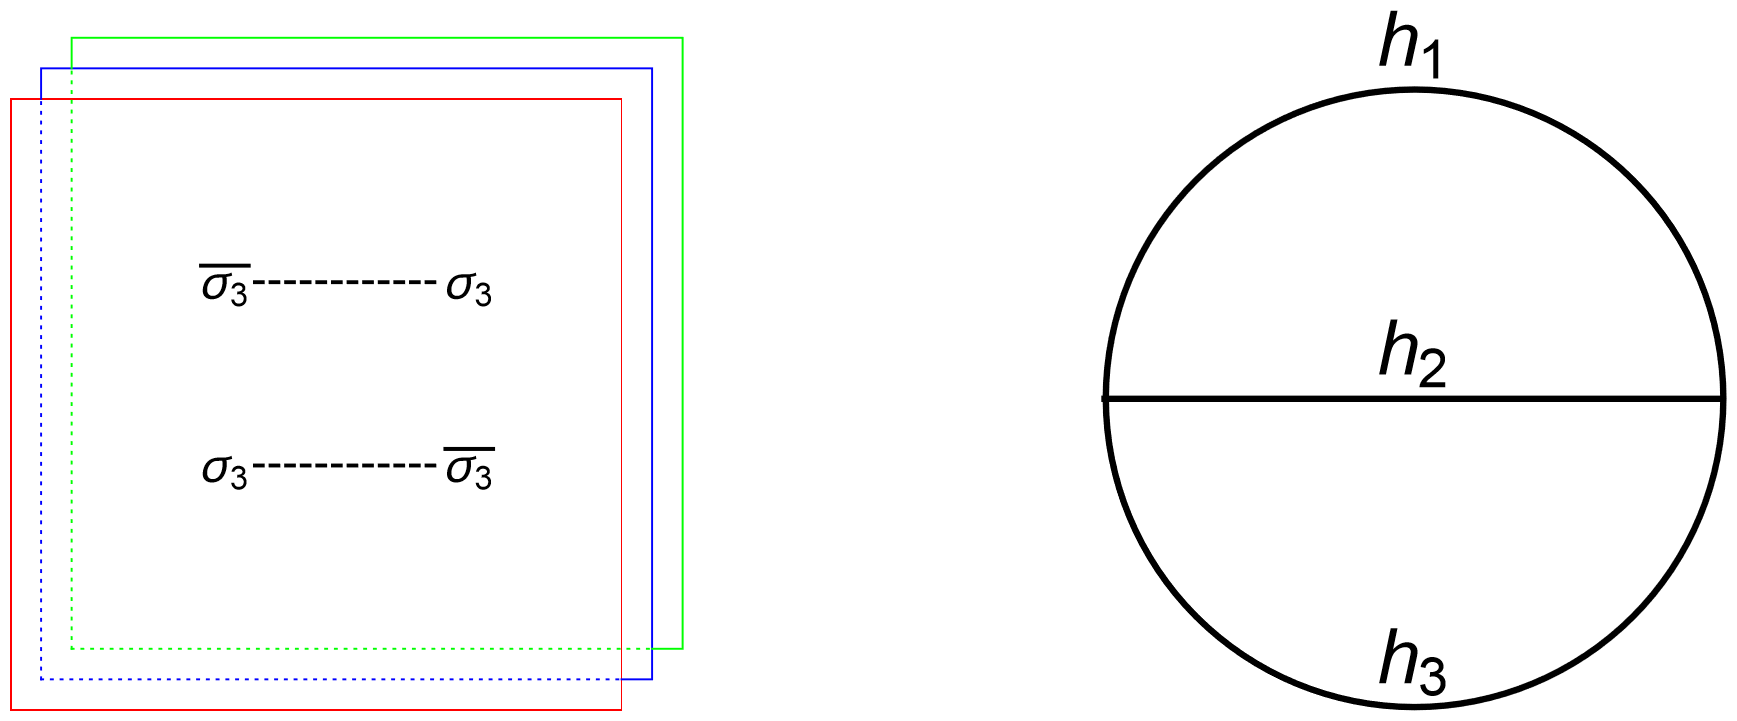
\includegraphics[width=0.85\textwidth]{figures/fig20.png}
  \caption{左：带四个分支点的黎曼球面的三折覆盖是亏格二曲面。覆盖曲面上 CFT 的配分函数可看作球面上三折对称积 CFT 中 $Z_3$ 扭曲场的四点函数。右：与 $\sigma_3\bar\sigma_3$ OPE 道相联系的亏格二共形块。（原文 p.47，图 20）}
  \label{fig:20}
\end{figure}

我们从“Rényi 曲面”出发：它是亏格二黎曼面模空间中的一条复一维轨迹，即黎曼球面在四个分支点处的三折覆盖。明确地说，可把 Rényi 曲面实现为 $\mathbb{CP}^1\times\mathbb{CP}^1$ 中的一条曲线，用仿射坐标 $(x,y)$ 写为
\begin{equation}
  \label{eq:5-42}
  y^3 = \frac{(x-x_1^+)(x-x_2^+)}
             {(x-x_1^-)(x-x_2^-)}.
\end{equation}
在由覆盖映射指定的特定共形框架下，Rényi 曲面上的亏格二配分函数等于黎曼球面上三重对称积 CFT 中一对 $Z_3$ 扭曲场 $\sigma_3$ 与一对反扭曲场 $\bar\sigma_3$ 的四点函数
\begin{equation}
  \label{eq:5-43}
  \bigl\langle \sigma_3(x_1^+)\sigma_3(x_2^+)
    \bar\sigma_3(x_1^-)\bar\sigma_3(x_2^-)\bigr\rangle,
\end{equation}
其亏格二共形块分解为
\begin{equation}
  \label{eq:5-44}
  \bigl\langle \sigma_3(0)\bar\sigma_3(z,\bar z)
    \sigma_3(1)\bar\sigma_3'(\infty)\bigr\rangle
  = \sum_{i,j,k} C_{ijk}^2\,
    \mathcal{F}_c(h_i,h_j,h_k;z)\,
    \overline{\mathcal{F}}_c
      (\tilde h_i,\tilde h_j,\tilde h_k;\bar z),
\end{equation}
其中共形块 $\mathcal{F}_c(h_i,h_j,h_k;z)$ 可通过直接对 $\sigma_3\bar\sigma_3$ OPE 中 Virasoro$^{\otimes 3}$ 后代的贡献求和，按 $z$ 展开计算。Rényi 框架共形块与 Rényi 曲面（仍由同一交比 $z$ 参数化）的管道框架块 $\mathcal{G}_c$ 相差一个共形反常因子：

% [Tutor Note: (5.44) 中的外权是扭曲场的权：对 $Z_3$ 覆盖，$\sigma_3$ 的共形权为 $h_\sigma=\frac{c}{24}(3-\frac13)=\frac{c}{9}$（$Z_2$ 覆盖时为 $\frac{c}{16}$）；代入 (5.47) 时要把 $h_1+h_2+h_3$ 取成 $3h_\sigma$，而不是 $0$。]

% ===== 原书 p.48（PDF 49）=====

\begin{equation}
  \label{eq:5-45}
  \mathcal{F}_c(h_1,h_2,h_3;z)
  = \exp\bigl[c\,\mathcal{F}^{cl}(z)\bigr]\,
    \mathcal{G}_c(h_1,h_2,h_3;z).
\end{equation}
这里记下 $\mathcal{F}^{cl}$ 的 $z$-展开前几项：
\begin{equation}
  \label{eq:5-46}
  \begin{aligned}
    \mathcal{F}^{cl}(z)
    = {}& -\frac{2}{9}\log(z)
      + 6\left(\frac{z}{27}\right)^2
      + 162\left(\frac{z}{27}\right)^3
      + 3975\left(\frac{z}{27}\right)^4\\
      & + 96552\left(\frac{z}{27}\right)^5
      + 2356039\left(\frac{z}{27}\right)^6
      + \cdots,
  \end{aligned}
\end{equation}
以及一般权 $h_1,h_2,h_3$ 下 $\mathcal{G}_c$ 的 $c\to\infty$ 极限：
\begin{equation}
  \label{eq:5-47}
  \begin{aligned}
    &\mathcal{G}_\infty(h_1,h_2,h_3;z)\\
    &\quad = \left(\frac{z}{27}\right)^{h_1+h_2+h_3}
    \left\{ 1 + \left[
      \frac{h_1+h_2+h_3}{2}
      + \frac{(h_2-h_3)^2}{54h_1}
      + \frac{(h_3-h_1)^2}{54h_2}
      + \frac{(h_1-h_2)^2}{54h_3}\right] z
      + \cdots\right\}.
  \end{aligned}
\end{equation}
若某个 $h_i$（比如 $h_3$）为零，对应真空道，则共形块只在 $h_1=h_2$ 时存在，并由一般块的 $h_3\to0$ 极限（取 $h_1=h_2$ 相等且为正）给出。$h_1=h_2=h_3=0$ 的真空块是特殊的，并不等于一般块的 $h_i\to0$ 极限，因为后者会错误地包含零态的贡献。

% [Tutor Note: (5.46) 的展开从 $(z/27)^2$ 开始、没有一次项，$\log z$ 的系数是 $-\frac29$；与 (5.47) 对照：$h_i\to0$ 时 (5.47) 的领头项为 $1$，正对应 (5.46) 的常数项为零。(5.47) 中的 $1/(54h_i)$ 在 $h_i\to0$ 时发散，可见这个极限是奇异的；正文随即指出它会错误地包含零态贡献，故真空块要单独处理。]

Rényi 曲面的亏格二共形块也可映射到三折枕形框架：
\begin{equation}
  \label{eq:5-48}
  \mathcal{F}_c(h_1,h_2,h_3;z)
  = \bigl(z(1-z)\bigr)^{-\frac{7c}{72}}
    \bigl(\theta_3(\tau)\bigr)^{-\frac{5}{18}}
    q^{h_1+h_2+h_3-\frac{c}{8}}
    \sum_{n=0}^{\infty} A_n(h_1,h_2,h_3)\,q^n,
\end{equation}
其中 $q=e^{\pi i\tau(z)}$ 是椭圆 nome，系数 $A_n(h_1,h_2,h_3)$ 在幺正性界限满足时为正。

% [Tutor Note: (5.48) 的三个指数 $-\frac{7c}{72}$、$-\frac{5}{18}$、$-\frac{c}{8}$ 中，$-\frac{5}{18}$ 是常数指数，另两个才依赖 $c$；抄录时最容易漏掉 $q$ 幂次上的 $-\frac{c}{8}$。]

我们可以像分析球面四点函数那样，在 $z=\bar z=\frac12$ 附近展开，来分析~\eqref{eq:5-44} 的 $z\to1-z$ 交叉对称性。作为一个简单但不平凡的例子，只用 $z$ 与 $\bar z$ 的一阶导数，交叉方程就蕴含维数三元组 $(\Delta_1,\Delta_2,\Delta_3)$ 空间中的一个临界区域 $D$：若 $(\Delta_i,\Delta_j,\Delta_k)$ 落在 $D$ 之外，相应的 OPE 系数 $C_{ijk}$ 就受落于 $D$ 内的权所对应系数的限制。图~\ref{fig:21} 给出一例。

\begin{figure}[htbp]
  \centering
  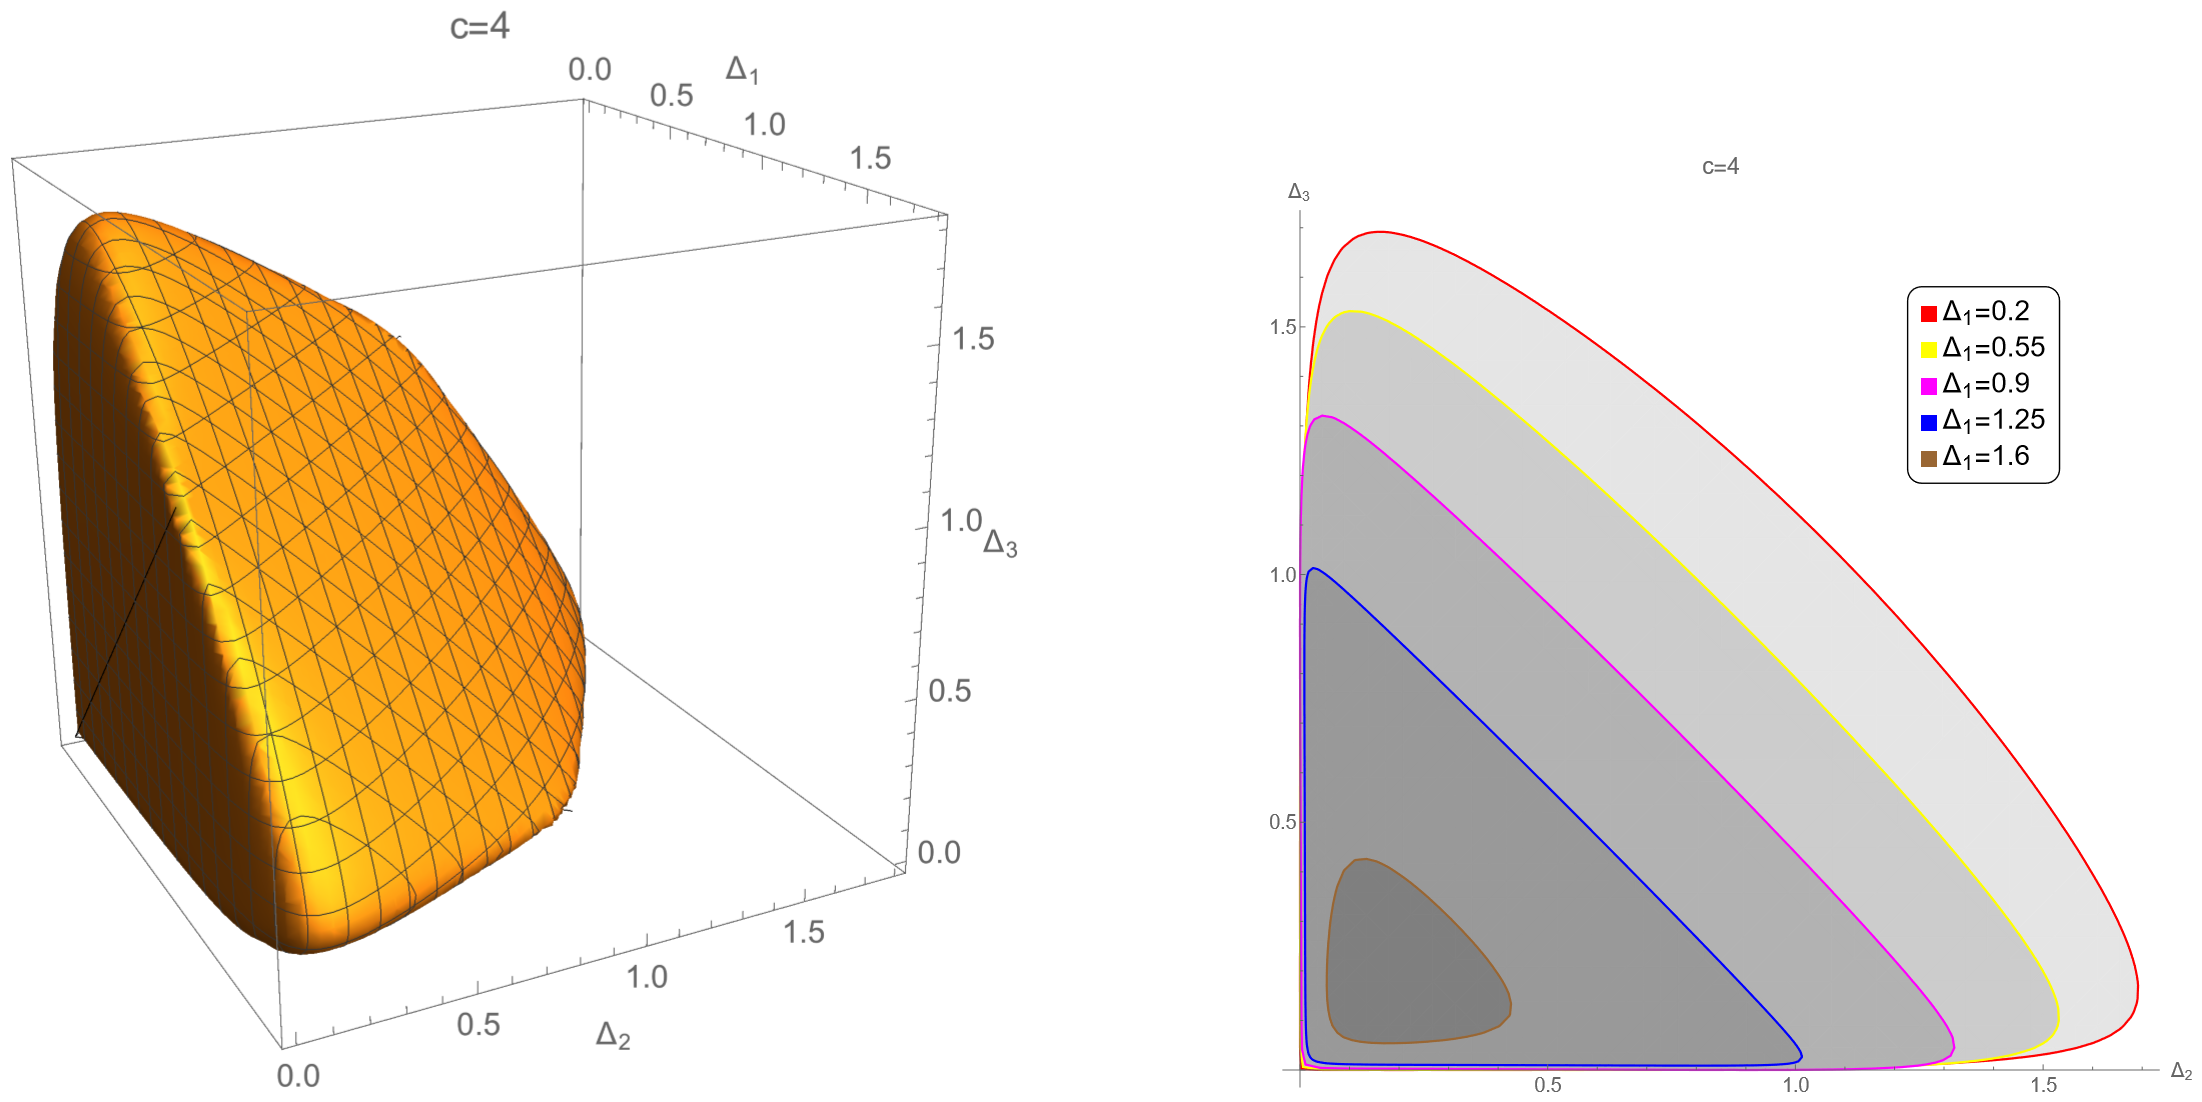
\includegraphics[width=0.85\textwidth]{figures/fig21.png}
  \caption{左：$c=4$ 时区域 $D_\Delta^{(3)}$ 的三维图。右：该区域在 $\Delta_1$ 取常数时的截面。图取自~\cite{r68}。（原文 p.49，图 21）}
  \label{fig:21}
\end{figure}

为偏离 Rényi 曲面，与其改变几何，不如在覆盖黎曼球面的三页中的任意一页插入能动张量 $T(z)$，或更一般的单位算符的 Virasoro 后代 $L_{-n_1}\cdots L_{-n_k}$。这样便能写出一般模的亏格二块在 Rényi 轨迹附近的展开，从而对 $C_{ijk}^2$ 表述完整的亏格二模交叉方程组。

% ===== 原书 p.48 末至 p.50（PDF 49--50）：第 6 章与致谢 =====

\section{总结}
\label{sec:6}

\begin{keytakeaways}
  \item 核心物理图像：可解的二维 CFT 仍局限于自由或有理理论、少数非紧致陪集模型及其轨形；一般二维 CFT 的完整自举方程组虽已写出，却仍无法实际求解。
  \item 使用的数学工具：交叉对称性与模不变性（环面一点函数的模协变、亏格二配分函数的模不变）给出的完整相容关系，以及半正定规划、线性泛函等数值手段。
  \item 本节结论：要刻画一般二维 CFT，必须把大量原初的 OPE 与模协变约束组织成具有正性的方程组（如亏格二模自举）；对非有理、紧致、相互作用的 CFT，目前的构造能力仍极为有限。
\end{keytakeaways}

过去四十年间，二维 CFT 方面积累了相当多的知识。然而，可解的二维 CFT 大体上仍局限于自由理论或有理理论、少数几个非紧致陪集模型，以及它们的轨形。

即便最简单的一类有理 CFT，即亚纯（meromorphic）CFT，也远未被分类：用配分函数的模不变性约束其谱很容易；但要证明存在一组结构常数，满足全部交叉方程与模协变的环面一点函数（不借助额外输入，例如对称性假设~\cite{r69}），却相当困难。

我们对相互作用、紧致、非有理 CFT 的了解少得令人难堪：唯一稳健的构造都基于 $(2,2)$ 超共形理论的精确边缘形变。迄今我们还不知道任何一个幺正、紧致 CFT 的例子，能在 Virasoro 对称性之外不含额外的高自旋守恒流。\footnote{临界耦合 Potts 模型~\cite{r54} 是一个潜在候选，但据我所知，它是否等价于某个已知的有理陪集模型，尚未被排除。}因此，要么我们漏掉了重要的约束（例如：$\frac{c-1}{12}$ 真的是扭曲间隙的最优上界吗~\cite{r58}？），要么我们对一般的二维 CFT 长什么样毫无头绪。显然，我们才刚刚开始开辟二维 CFT 的版图，未来数十年还有大量东西要学。

% [Tutor Note: 正文把上界写作 $\frac{c-1}{12}$ 而不是 $\frac{c}{12}$：分子里的 $-1$ 使该界略低于 $c/12$，来自真空态（模不变真空特征标）的贡献；引用 \cite{r58} 时勿把分子写成 $c$。]

\section*{致谢}

感谢 TASI 2017 的组织者邀请我，也感谢参加的学生们的热情与富有启发性的问题。感谢 Chi-Ming Chang、Minjae Cho、Scott Collier、Petr Kravchuk、Ying-Hsuan Lin、Shu-Heng Shao、David Simmons-Duffin、Yifan Wang 的合作，以及 Thomas Dumitrescu、Daniel Harlow、Simeon Hellerman、Christoph Keller、Zohar Komargodski、Alex Maloney、Eric Perlmutter、Slava Rychkov、Ashoke Sen、Andy Strominger、Cumrun Vafa 的有益讨论。本工作由 Simons Foundation 的 Simons Investigator Award 与 DOE 基金 DE-FG02-91ER40654 支持。

% 以下为参考文献（References），由参考文献译者负责，本文件在此停止。


% References —— 原书 p.49--53（PDF 第 50--54 页）
% 底本：Xi Yin, Aspects of Two-Dimensional Conformal Field Theories, PoS(TASI2017)003
% 条目按原文编号 [1]--[69] 顺序排列，作者名与英文标题保留原文，不翻译。
% 编号由 \bibitem 自动生成，故 r1..r69 必须连续。

\begin{thebibliography}{99}

\bibitem{r1} G.~W. Moore and N. Seiberg, \emph{Classical and Quantum Conformal Field Theory}, Commun.\ Math.\ Phys.\ \textbf{123} (1989) 177.

\bibitem{r2} V.~G. Kac and D.~A. Kazhdan, \emph{Structure of representations with highest weight of infinite dimensional Lie algebras}, Adv.\ Math.\ \textbf{34} (1979) 97--108.

\bibitem{r3} B.~L. Feigin and D.~B. Fuchs, \emph{VERMA MODULES OVER THE VIRASORO ALGEBRA}, .
% [Tutor Note: 原文该条在此处即终止，仅剩一个逗号和一个句点；期刊名、卷、年、页码全部缺失（底本 PDF p.50 印刷残缺），非本次转录遗漏。]

\bibitem{r4} D. Friedan, Z.-a. Qiu, and S.~H. Shenker, \emph{Conformal Invariance, Unitarity and Two-Dimensional Critical Exponents}, Phys.\ Rev.\ Lett.\ \textbf{52} (1984) 1575--1578.

\bibitem{r5} P. Di Francesco, P. Mathieu, and D. S\'en\'echal, \emph{Conformal field theory}. Graduate texts in contemporary physics. Springer, New York, NY, 1997.

\bibitem{r6} D. Buchholz, S. Doplicher, and R. Longo, \emph{On Noether's Theorem in Quantum Field Theory}, Annals Phys.\ \textbf{170} (1986) 1.

\bibitem{r7} D. Harlow, \emph{The Ryu-Takayanagi Formula from Quantum Error Correction}, arXiv:1607.03901.

\bibitem{r8} D. Whalen, \emph{An algorithm for evaluating Gram matrices in Verma modules of $W$-algebras}, arXiv:1412.0759.

\bibitem{r9} A.~B. Zamolodchikov, \emph{Conformal symmetry in two-dimensions: an explicit recurrence formula for the conformal partial wave amplitude}, Commun.\ Math.\ Phys.\ \textbf{96} (1984) 419--422.

\bibitem{r10} A.~B. Zamolodchikov, \emph{Conformal symmetry in two-dimensional space: Recursion representation of conformal block}, Theoretical and Mathematical Physics \textbf{73} (Oct., 1987) 1088--1093.

\bibitem{r11} J. Maldacena, D. Simmons-Duffin, and A. Zhiboedov, \emph{Looking for a bulk point}, arXiv:1509.03612.

\bibitem{r12} H. Dorn and H.~J. Otto, \emph{Two and three point functions in Liouville theory}, Nucl.\ Phys.\ \textbf{B429} (1994) 375--388, [hep-th/9403141].

\bibitem{r13} A.~B. Zamolodchikov and A.~B. Zamolodchikov, \emph{Structure constants and conformal bootstrap in Liouville field theory}, Nucl.\ Phys.\ \textbf{B477} (1996) 577--605, [hep-th/9506136].

\bibitem{r14} B. Ponsot and J. Teschner, \emph{Liouville bootstrap via harmonic analysis on a noncompact quantum group}, hep-th/9911110.

\bibitem{r15} J. Teschner, \emph{Liouville theory revisited}, Class.\ Quant.\ Grav.\ \textbf{18} (2001) R153--R222, [hep-th/0104158].

\bibitem{r16} L. Hadasz, Z. Jaskolski, and P. Suchanek, \emph{Modular bootstrap in Liouville field theory}, Phys.\ Lett.\ \textbf{B685} (2010) 79--85, [arXiv:0911.4296].

\bibitem{r17} N. Seiberg, \emph{Notes on quantum Liouville theory and quantum gravity}, Prog.\ Theor.\ Phys.\ Suppl.\ \textbf{102} (1990) 319--349.

\bibitem{r18} K.~S. Narain, \emph{New Heterotic String Theories in Uncompactified Dimensions $<10$}, Phys.\ Lett.\ \textbf{B169} (1986) 41--46.

\bibitem{r19} L.~J. Dixon, D. Friedan, E.~J. Martinec, and S.~H. Shenker, \emph{The Conformal Field Theory of Orbifolds}, Nucl.\ Phys.\ \textbf{B282} (1987) 13--73.

\bibitem{r20} I. Frenkel, J. Lepowsky, and A. Meurman, \emph{VERTEX OPERATOR ALGEBRAS AND THE MONSTER}. 1988.
% [Tutor Note: 该条为专著（Academic Press, 1988），原文只给书名与年份，未给出版社与丛书信息。]

\bibitem{r21} E. Witten, \emph{Nonabelian Bosonization in Two-Dimensions}, Commun.\ Math.\ Phys.\ \textbf{92} (1984) 455--472.

\bibitem{r22} D. Gepner and E. Witten, \emph{String Theory on Group Manifolds}, Nucl.\ Phys.\ \textbf{B278} (1986) 493--549.

\bibitem{r23} P. Goddard, A. Kent, and D.~I. Olive, \emph{Unitary Representations of the Virasoro and Supervirasoro Algebras}, Commun.\ Math.\ Phys.\ \textbf{103} (1986) 105--119.

\bibitem{r24} K. Gawedzki and A. Kupiainen, \emph{$G/h$ Conformal Field Theory from Gauged WZW Model}, Phys.\ Lett.\ \textbf{B215} (1988) 119--123.

\bibitem{r25} C.~G. Callan, Jr. and L. Thorlacius, \emph{SIGMA MODELS AND STRING THEORY}, in \emph{Theoretical Advanced Study Institute in Elementary Particle Physics: Particles, Strings and Supernovae (TASI 88)} Providence, Rhode Island, June 5-July 1, 1988, pp.~795--878, 1989.

\bibitem{r26} F. Gliozzi, J. Scherk, and D.~I. Olive, \emph{Supersymmetry, Supergravity Theories and the Dual Spinor Model}, Nucl.\ Phys.\ \textbf{B122} (1977) 253--290.

\bibitem{r27} S. Odake, \emph{Extension of $N=2$ Superconformal Algebra and Calabi-yau Compactification}, Mod.\ Phys.\ Lett.\ \textbf{A4} (1989) 557.

\bibitem{r28} S. Odake, \emph{$C=3-d$ Conformal Algebra With Extended Supersymmetry}, Mod.\ Phys.\ Lett.\ \textbf{A5} (1990) 561.

\bibitem{r29} D. Kutasov, \emph{Some properties of (non)critical strings}, in \emph{Spring School on String Theory and Quantum Gravity (to be followed by Workshop)} Trieste, Italy, April 15-23, 1991, pp.~102--141, 1991. hep-th/9110041.

\bibitem{r30} T. Eguchi and A. Taormina, \emph{Unitary Representations of $N=4$ Superconformal Algebra}, Phys.\ Lett.\ \textbf{B196} (1987) 75.

\bibitem{r31} C. Kounnas, M. Porrati, and B. Rostand, \emph{ON $N=4$ extended superLiouville theory}, Phys.\ Lett.\ \textbf{B258} (1991) 61--69.

\bibitem{r32} T. Eguchi and A. Taormina, \emph{On the Unitary Representations of $N=2$ and $N=4$ Superconformal Algebras}, Phys.\ Lett.\ \textbf{B210} (1988) 125.

\bibitem{r33} W. Boucher, D. Friedan, and A. Kent, \emph{Determinant Formulae and Unitarity for the $N=2$ Superconformal Algebras in Two-Dimensions or Exact Results on String Compactification}, Phys.\ Lett.\ \textbf{B172} (1986) 316.

\bibitem{r34} E. Witten, \emph{Elliptic Genera and Quantum Field Theory}, Commun.\ Math.\ Phys.\ \textbf{109} (1987) 525.

\bibitem{r35} T. Eguchi, H. Ooguri, A. Taormina, and S.-K. Yang, \emph{Superconformal Algebras and String Compactification on Manifolds with $SU(N)$ Holonomy}, Nucl.\ Phys.\ \textbf{B315} (1989) 193.

\bibitem{r36} A.~B. Zamolodchikov, \emph{Irreversibility of the Flux of the Renormalization Group in a 2D Field Theory}, JETP Lett.\ \textbf{43} (1986) 730--732. [Pisma Zh.\ Eksp.\ Teor.\ Fiz.\ 43, 565 (1986)].

\bibitem{r37} L.~J. Dixon, \emph{SOME WORLD SHEET PROPERTIES OF SUPERSTRING COMPACTIFICATIONS, ON ORBIFOLDS AND OTHERWISE}, in \emph{Summer Workshop in High-energy Physics and Cosmology} Trieste, Italy, June 29-August 7, 1987, 1987.

\bibitem{r38} D. Green, Z. Komargodski, N. Seiberg, Y. Tachikawa, and B. Wecht, \emph{Exactly Marginal Deformations and Global Symmetries}, JHEP \textbf{06} (2010) 106, [arXiv:1005.3546].

\bibitem{r39} R. Dijkgraaf, \emph{Instanton strings and hyperKahler geometry}, Nucl.\ Phys.\ \textbf{B543} (1999) 545--571, [hep-th/9810210].

\bibitem{r40} N. Seiberg and E. Witten, \emph{The $D1/D5$ system and singular CFT}, JHEP \textbf{04} (1999) 017, [hep-th/9903224].

\bibitem{r41} F. Larsen and E.~J. Martinec, \emph{$U(1)$ charges and moduli in the $D1$ - $D5$ system}, JHEP \textbf{06} (1999) 019, [hep-th/9905064].

\bibitem{r42} A.~B. Zamolodchikov, \emph{Thermodynamic Bethe Ansatz in Relativistic Models. Scaling Three State Potts and Lee-yang Models}, Nucl.\ Phys.\ \textbf{B342} (1990) 695--720.

\bibitem{r43} A.~B. Zamolodchikov, \emph{TBA equations for integrable perturbed $SU(2)$-$k$ $\times$ $SU(2)$-$l$ / $SU(2)$-$k+l$ coset models}, Nucl.\ Phys.\ \textbf{B366} (1991) 122--132.

\bibitem{r44} A.~B. Zamolodchikov, \emph{Thermodynamic Bethe ansatz for RSOS scattering theories}, Nucl.\ Phys.\ \textbf{B358} (1991) 497--523.

\bibitem{r45} A.~B. Zamolodchikov, \emph{From tricritical Ising to critical Ising by thermodynamic Bethe ansatz}, Nucl.\ Phys.\ \textbf{B358} (1991) 524--546.

\bibitem{r46} A.~B. Zamolodchikov, \emph{On the thermodynamic Bethe ansatz equations for reflectionless ADE scattering theories}, Phys.\ Lett.\ \textbf{B253} (1991) 391--394.

\bibitem{r47} A.~B. Zamolodchikov, \emph{On the thermodynamic Bethe ansatz equation in sinh-Gordon model}, J.\ Phys.\ \textbf{A39} (2006) 12863--12887, [hep-th/0005181].

\bibitem{r48} M. Karowski and P. Weisz, \emph{Exact Form-Factors in (1+1)-Dimensional Field Theoretic Models with Soliton Behavior}, Nucl.\ Phys.\ \textbf{B139} (1978) 455--476.

\bibitem{r49} H.~M. Babujian, A. Foerster, and M. Karowski, \emph{The form factor program: A review and new results, the nested $SU(N)$ off-shell Bethe ansatz and the $1/N$ expansion}, Theor.\ Math.\ Phys.\ \textbf{155} (2008) 512--522. [Teor.\ Mat.\ Fiz.\ 155, 13 (2008)].

\bibitem{r50} V.~P. Yurov and A.~B. Zamolodchikov, \emph{TRUNCATED CONFORMAL SPACE APPROACH TO SCALING LEE-YANG MODEL}, Int.\ J.\ Mod.\ Phys.\ \textbf{A5} (1990) 3221--3246.

\bibitem{r51} V.~P. Yurov and A.~B. Zamolodchikov, \emph{Truncated fermionic space approach to the critical 2-D Ising model with magnetic field}, Int.\ J.\ Mod.\ Phys.\ \textbf{A6} (1991) 4557--4578.

\bibitem{r52} S. Rychkov and L.~G. Vitale, \emph{Hamiltonian truncation study of the $\phi^4$ theory in two dimensions}, Phys.\ Rev.\ \textbf{D91} (2015) 085011, [arXiv:1412.3460].
% [Tutor Note: 底本该条标题中 $\phi$ 字符未渲染，印刷上只见上标 4（"... study of the $^{4}$ theory ..."）。此处按文献通行题目补为 $\phi^4$；核对时以 Phys. Rev. D91 (2015) 085011 原题为准。]

\bibitem{r53} B.~R. Greene, C. Vafa, and N.~P. Warner, \emph{Calabi-Yau Manifolds and Renormalization Group Flows}, Nucl.\ Phys.\ \textbf{B324} (1989) 371.

\bibitem{r54} V. Dotsenko, J.~L. Jacobsen, M.-A. Lewis, and M. Picco, \emph{Coupled Potts models: Self-duality and fixed point structure}, Nucl.\ Phys.\ \textbf{B546} (1999) 505--557.

\bibitem{r55} E. Witten, \emph{Phases of $N=2$ theories in two-dimensions}, Nucl.\ Phys.\ \textbf{B403} (1993) 159--222, [hep-th/9301042].

\bibitem{r56} S. Hellerman, \emph{A Universal Inequality for CFT and Quantum Gravity}, JHEP \textbf{08} (2011) 130, [arXiv:0902.2790].

\bibitem{r57} D. Friedan and C.~A. Keller, \emph{Constraints on 2d CFT partition functions}, JHEP \textbf{10} (2013) 180, [arXiv:1307.6562].

\bibitem{r58} S. Collier, Y.-H. Lin, and X. Yin, \emph{Modular Bootstrap Revisited}, arXiv:1608.06241.

\bibitem{r59} S. El-Showk and M.~F. Paulos, \emph{Bootstrapping Conformal Field Theories with the Extremal Functional Method}, Phys.\ Rev.\ Lett.\ \textbf{111} (2013), no.~24 241601, [arXiv:1211.2810].

\bibitem{r60} S. El-Showk, M.~F. Paulos, D. Poland, S. Rychkov, D. Simmons-Duffin, and A. Vichi, \emph{Solving the 3d Ising Model with the Conformal Bootstrap II. $c$-Minimization and Precise Critical Exponents}, J.\ Stat.\ Phys.\ \textbf{157} (2014) 869, [arXiv:1403.4545].

\bibitem{r61} S. Collier, P. Kravchuk, Y.-H. Lin, and X. Yin, \emph{Bootstrapping the Spectral Function: On the Uniqueness of Liouville and the Universality of BTZ}, arXiv:1702.00423.

\bibitem{r62} E. Kiritsis, N.~A. Obers, and B. Pioline, \emph{Heterotic / type II triality and instantons on $K(3)$}, JHEP \textbf{01} (2000) 029, [hep-th/0001083].

\bibitem{r63} Y.-H. Lin, S.-H. Shao, Y. Wang, and X. Yin, \emph{Supersymmetry Constraints and String Theory on $K3$}, arXiv:1508.07305.

\bibitem{r64} Y.-H. Lin, S.-H. Shao, D. Simmons-Duffin, Y. Wang, and X. Yin, \emph{$N=4$ Superconformal Bootstrap of the $K3$ CFT}, arXiv:1511.04065.

\bibitem{r65} Y.-H. Lin, S.-H. Shao, Y. Wang, and X. Yin, \emph{(2,2) Superconformal Bootstrap in Two Dimensions}, arXiv:1610.05371.

\bibitem{r66} P. Candelas, X.~C. De La Ossa, P.~S. Green, and L. Parkes, \emph{A Pair of Calabi-Yau manifolds as an exactly soluble superconformal theory}, Nucl.\ Phys.\ \textbf{B359} (1991) 21--74.

\bibitem{r67} S. Giombi, A. Maloney, and X. Yin, \emph{One-loop Partition Functions of 3D Gravity}, JHEP \textbf{08} (2008) 007, [arXiv:0804.1773].

\bibitem{r68} M. Cho, S. Collier, and X. Yin, \emph{Genus Two Modular Bootstrap}, arXiv:1705.05865.

\bibitem{r69} D. Gaiotto, \emph{Monster symmetry and Extremal CFTs}, arXiv:0801.0988.

\end{thebibliography}


\end{document}


